\PassOptionsToPackage{unicode=true}{hyperref} % options for packages loaded elsewhere
\PassOptionsToPackage{hyphens}{url}
%
\documentclass[]{book}
\usepackage{lmodern}
\usepackage{amssymb,amsmath}
\usepackage{ifxetex,ifluatex}
\usepackage{fixltx2e} % provides \textsubscript
\ifnum 0\ifxetex 1\fi\ifluatex 1\fi=0 % if pdftex
  \usepackage[T1]{fontenc}
  \usepackage[utf8]{inputenc}
  \usepackage{textcomp} % provides euro and other symbols
\else % if luatex or xelatex
  \usepackage{unicode-math}
  \defaultfontfeatures{Ligatures=TeX,Scale=MatchLowercase}
\fi
% use upquote if available, for straight quotes in verbatim environments
\IfFileExists{upquote.sty}{\usepackage{upquote}}{}
% use microtype if available
\IfFileExists{microtype.sty}{%
\usepackage[]{microtype}
\UseMicrotypeSet[protrusion]{basicmath} % disable protrusion for tt fonts
}{}
\IfFileExists{parskip.sty}{%
\usepackage{parskip}
}{% else
\setlength{\parindent}{0pt}
\setlength{\parskip}{6pt plus 2pt minus 1pt}
}
\usepackage{hyperref}
\hypersetup{
            pdftitle={Technical Interview},
            pdfauthor={Michael Fong},
            pdfborder={0 0 0},
            breaklinks=true}
\urlstyle{same}  % don't use monospace font for urls
\usepackage{color}
\usepackage{fancyvrb}
\newcommand{\VerbBar}{|}
\newcommand{\VERB}{\Verb[commandchars=\\\{\}]}
\DefineVerbatimEnvironment{Highlighting}{Verbatim}{commandchars=\\\{\}}
% Add ',fontsize=\small' for more characters per line
\usepackage{framed}
\definecolor{shadecolor}{RGB}{248,248,248}
\newenvironment{Shaded}{\begin{snugshade}}{\end{snugshade}}
\newcommand{\AlertTok}[1]{\textcolor[rgb]{0.94,0.16,0.16}{#1}}
\newcommand{\AnnotationTok}[1]{\textcolor[rgb]{0.56,0.35,0.01}{\textbf{\textit{#1}}}}
\newcommand{\AttributeTok}[1]{\textcolor[rgb]{0.77,0.63,0.00}{#1}}
\newcommand{\BaseNTok}[1]{\textcolor[rgb]{0.00,0.00,0.81}{#1}}
\newcommand{\BuiltInTok}[1]{#1}
\newcommand{\CharTok}[1]{\textcolor[rgb]{0.31,0.60,0.02}{#1}}
\newcommand{\CommentTok}[1]{\textcolor[rgb]{0.56,0.35,0.01}{\textit{#1}}}
\newcommand{\CommentVarTok}[1]{\textcolor[rgb]{0.56,0.35,0.01}{\textbf{\textit{#1}}}}
\newcommand{\ConstantTok}[1]{\textcolor[rgb]{0.00,0.00,0.00}{#1}}
\newcommand{\ControlFlowTok}[1]{\textcolor[rgb]{0.13,0.29,0.53}{\textbf{#1}}}
\newcommand{\DataTypeTok}[1]{\textcolor[rgb]{0.13,0.29,0.53}{#1}}
\newcommand{\DecValTok}[1]{\textcolor[rgb]{0.00,0.00,0.81}{#1}}
\newcommand{\DocumentationTok}[1]{\textcolor[rgb]{0.56,0.35,0.01}{\textbf{\textit{#1}}}}
\newcommand{\ErrorTok}[1]{\textcolor[rgb]{0.64,0.00,0.00}{\textbf{#1}}}
\newcommand{\ExtensionTok}[1]{#1}
\newcommand{\FloatTok}[1]{\textcolor[rgb]{0.00,0.00,0.81}{#1}}
\newcommand{\FunctionTok}[1]{\textcolor[rgb]{0.00,0.00,0.00}{#1}}
\newcommand{\ImportTok}[1]{#1}
\newcommand{\InformationTok}[1]{\textcolor[rgb]{0.56,0.35,0.01}{\textbf{\textit{#1}}}}
\newcommand{\KeywordTok}[1]{\textcolor[rgb]{0.13,0.29,0.53}{\textbf{#1}}}
\newcommand{\NormalTok}[1]{#1}
\newcommand{\OperatorTok}[1]{\textcolor[rgb]{0.81,0.36,0.00}{\textbf{#1}}}
\newcommand{\OtherTok}[1]{\textcolor[rgb]{0.56,0.35,0.01}{#1}}
\newcommand{\PreprocessorTok}[1]{\textcolor[rgb]{0.56,0.35,0.01}{\textit{#1}}}
\newcommand{\RegionMarkerTok}[1]{#1}
\newcommand{\SpecialCharTok}[1]{\textcolor[rgb]{0.00,0.00,0.00}{#1}}
\newcommand{\SpecialStringTok}[1]{\textcolor[rgb]{0.31,0.60,0.02}{#1}}
\newcommand{\StringTok}[1]{\textcolor[rgb]{0.31,0.60,0.02}{#1}}
\newcommand{\VariableTok}[1]{\textcolor[rgb]{0.00,0.00,0.00}{#1}}
\newcommand{\VerbatimStringTok}[1]{\textcolor[rgb]{0.31,0.60,0.02}{#1}}
\newcommand{\WarningTok}[1]{\textcolor[rgb]{0.56,0.35,0.01}{\textbf{\textit{#1}}}}
\usepackage{longtable,booktabs}
% Fix footnotes in tables (requires footnote package)
\IfFileExists{footnote.sty}{\usepackage{footnote}\makesavenoteenv{longtable}}{}
\usepackage{graphicx,grffile}
\makeatletter
\def\maxwidth{\ifdim\Gin@nat@width>\linewidth\linewidth\else\Gin@nat@width\fi}
\def\maxheight{\ifdim\Gin@nat@height>\textheight\textheight\else\Gin@nat@height\fi}
\makeatother
% Scale images if necessary, so that they will not overflow the page
% margins by default, and it is still possible to overwrite the defaults
% using explicit options in \includegraphics[width, height, ...]{}
\setkeys{Gin}{width=\maxwidth,height=\maxheight,keepaspectratio}
\setlength{\emergencystretch}{3em}  % prevent overfull lines
\providecommand{\tightlist}{%
  \setlength{\itemsep}{0pt}\setlength{\parskip}{0pt}}
\setcounter{secnumdepth}{5}
% Redefines (sub)paragraphs to behave more like sections
\ifx\paragraph\undefined\else
\let\oldparagraph\paragraph
\renewcommand{\paragraph}[1]{\oldparagraph{#1}\mbox{}}
\fi
\ifx\subparagraph\undefined\else
\let\oldsubparagraph\subparagraph
\renewcommand{\subparagraph}[1]{\oldsubparagraph{#1}\mbox{}}
\fi

% set default figure placement to htbp
\makeatletter
\def\fps@figure{htbp}
\makeatother

\usepackage{booktabs}
\usepackage{amsthm}
\makeatletter
\def\thm@space@setup{%
  \thm@preskip=8pt plus 2pt minus 4pt
  \thm@postskip=\thm@preskip
}
\makeatother
\usepackage[]{natbib}
\bibliographystyle{apalike}

\title{Technical Interview}
\author{Michael Fong}
\date{2020-04-04}

\begin{document}
\maketitle

%\printindex
%\printglossaries

{
\setcounter{tocdepth}{1}
\tableofcontents
}
\hypertarget{intro}{%
\chapter{Introduction}\label{intro}}

You can label chapter and section titles using \texttt{\{\#label\}} after them, e.g., we can reference Chapter \ref{intro}. If you do not manually label them, there will be automatic labels anyway, e.g., Chapter \ref{methods}.

\hypertarget{glossary}{%
\section{Glossary}\label{glossary}}

\hypertarget{term1}{%
\subsection{Term 1}\label{term1}}

: This is a definition with two paragraphs. Lorem ipsum
dolor sit amet, consectetuer adipiscing elit. Aliquam
hendrerit mi posuere lectus.

\begin{verbatim}
Vestibulum enim wisi, viverra nec, fringilla in, laoreet
vitae, risus.
\end{verbatim}

: Second definition for term 1, also wrapped in a paragraph
because of the blank line preceding it.

\hypertarget{term2}{%
\subsection{Term 2}\label{term2}}

: This definition has a code block, a blockquote and a list.

\begin{verbatim}
    code block.

> block quote
> on two lines.

1.  first list item
2.  second list item
\end{verbatim}

Reference: Term 1 \ref{term1}.and Term 2 \ref{term2}

Figures and tables with captions will be placed in \texttt{figure} and \texttt{table} environments, respectively.

\begin{Shaded}
\begin{Highlighting}[]
\KeywordTok{par}\NormalTok{(}\DataTypeTok{mar =} \KeywordTok{c}\NormalTok{(}\DecValTok{4}\NormalTok{, }\DecValTok{4}\NormalTok{, }\FloatTok{.1}\NormalTok{, }\FloatTok{.1}\NormalTok{))}
\KeywordTok{plot}\NormalTok{(pressure, }\DataTypeTok{type =} \StringTok{'b'}\NormalTok{, }\DataTypeTok{pch =} \DecValTok{19}\NormalTok{)}
\end{Highlighting}
\end{Shaded}

\begin{figure}

{\centering 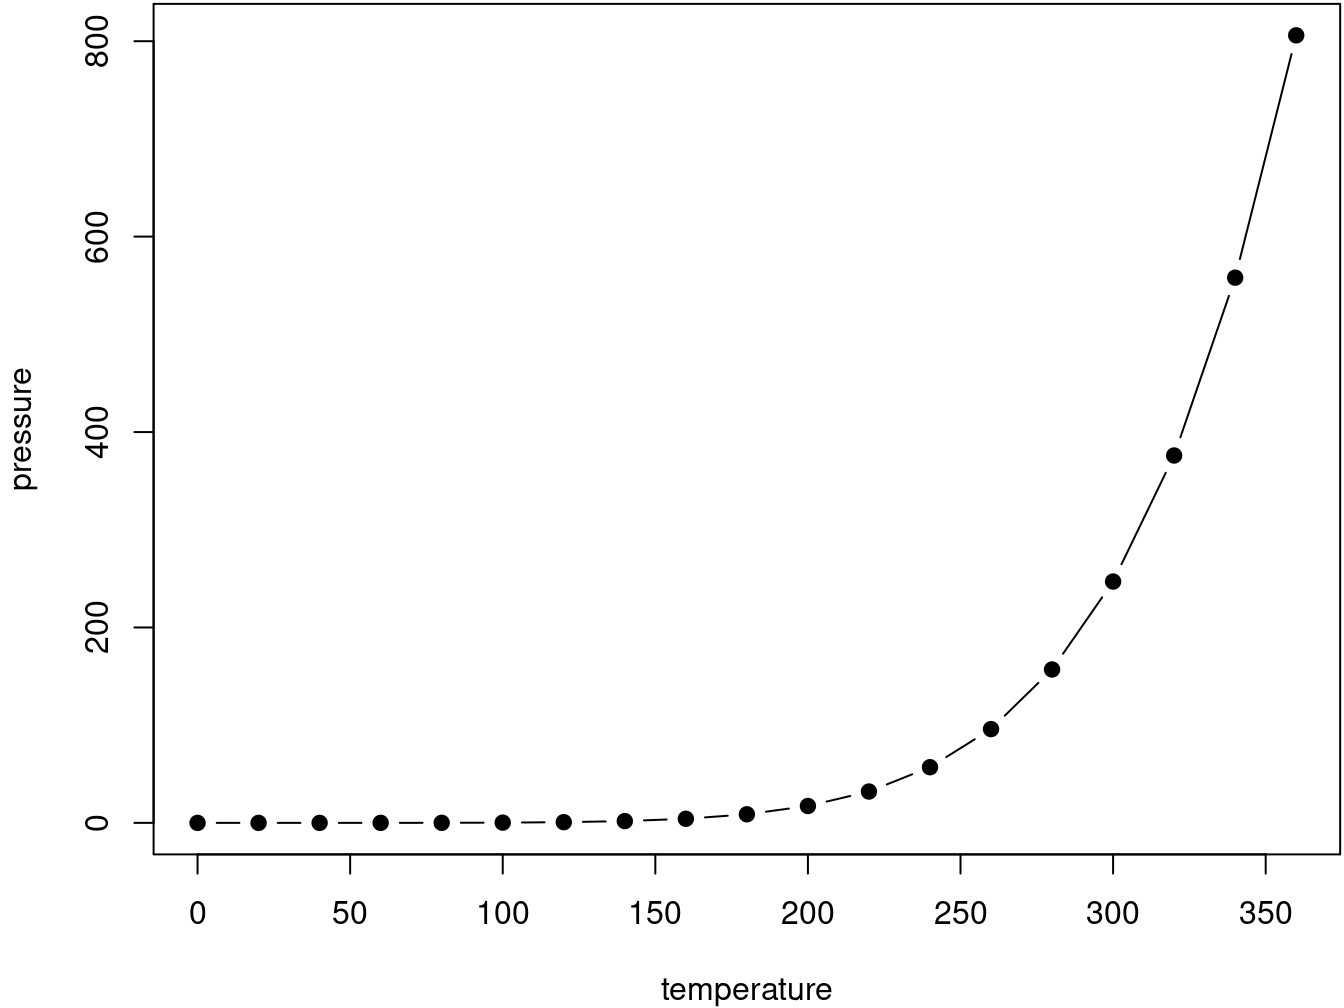
\includegraphics[width=0.8\linewidth]{bookdown-demo_files/figure-latex/nice-fig-1} 

}

\caption{Here is a nice figure!}\label{fig:nice-fig}
\end{figure}

Reference a figure by its code chunk label with the \texttt{fig:} prefix, e.g., see Figure \ref{fig:nice-fig}. Similarly, you can reference tables generated from \texttt{knitr::kable()}, e.g., see Table \ref{tab:nice-tab}.

\begin{Shaded}
\begin{Highlighting}[]
\NormalTok{knitr}\OperatorTok{::}\KeywordTok{kable}\NormalTok{(}
  \KeywordTok{head}\NormalTok{(iris, }\DecValTok{20}\NormalTok{), }\DataTypeTok{caption =} \StringTok{'Here is a nice table!'}\NormalTok{,}
  \DataTypeTok{booktabs =} \OtherTok{TRUE}
\NormalTok{)}
\end{Highlighting}
\end{Shaded}

\begin{table}

\caption{\label{tab:nice-tab}Here is a nice table!}
\centering
\begin{tabular}[t]{rrrrl}
\toprule
Sepal.Length & Sepal.Width & Petal.Length & Petal.Width & Species\\
\midrule
5.1 & 3.5 & 1.4 & 0.2 & setosa\\
4.9 & 3.0 & 1.4 & 0.2 & setosa\\
4.7 & 3.2 & 1.3 & 0.2 & setosa\\
4.6 & 3.1 & 1.5 & 0.2 & setosa\\
5.0 & 3.6 & 1.4 & 0.2 & setosa\\
\addlinespace
5.4 & 3.9 & 1.7 & 0.4 & setosa\\
4.6 & 3.4 & 1.4 & 0.3 & setosa\\
5.0 & 3.4 & 1.5 & 0.2 & setosa\\
4.4 & 2.9 & 1.4 & 0.2 & setosa\\
4.9 & 3.1 & 1.5 & 0.1 & setosa\\
\addlinespace
5.4 & 3.7 & 1.5 & 0.2 & setosa\\
4.8 & 3.4 & 1.6 & 0.2 & setosa\\
4.8 & 3.0 & 1.4 & 0.1 & setosa\\
4.3 & 3.0 & 1.1 & 0.1 & setosa\\
5.8 & 4.0 & 1.2 & 0.2 & setosa\\
\addlinespace
5.7 & 4.4 & 1.5 & 0.4 & setosa\\
5.4 & 3.9 & 1.3 & 0.4 & setosa\\
5.1 & 3.5 & 1.4 & 0.3 & setosa\\
5.7 & 3.8 & 1.7 & 0.3 & setosa\\
5.1 & 3.8 & 1.5 & 0.3 & setosa\\
\bottomrule
\end{tabular}
\end{table}

You can write citations, too. For example, we are using the \textbf{bookdown} package \citep{R-bookdown} in this sample book, which was built on top of R Markdown and \textbf{knitr} \citep{bookmark}.

\hypertarget{arrays}{%
\chapter{Arrays}\label{arrays}}

If we are enumerating the cartesian products over two arrays of n elements.

\begin{verbatim}
A = [A_1, A_2, ..., A_n]
B = [B_1, B_2, ..., B_n]
A1 X A2 = [(A_1, B_1), (A_1, B_2), ..., (A_n, B_n)]
\end{verbatim}

The time complexity is O(n\^{}2).

\begin{Shaded}
\begin{Highlighting}[]
\KeywordTok{for}\NormalTok{(}\DataTypeTok{int}\NormalTok{ i = }\DecValTok{0}\NormalTok{; i < A.}\FunctionTok{length}\NormalTok{; i++) \{}
    \KeywordTok{for}\NormalTok{(}\DataTypeTok{int}\NormalTok{ j = }\DecValTok{0}\NormalTok{; j < B.}\FunctionTok{length}\NormalTok{; j++) \{}
        \CommentTok{// process each (A_i, B_j)}
\NormalTok{    \}}
\NormalTok{\}}
\end{Highlighting}
\end{Shaded}

If we only need to enumerate part of the combination over two arrays while traversing both arrays simultaneously.

\begin{verbatim}
A = [A_1, A_2, ..., A_n]
B = [B_1, B_2, ..., B_n]
A1 X A2 = [(A_1, B_1), (A_2, B_1), (A_2, B_2), ..., (A_n, B_n)]
\end{verbatim}

we could possibly reduce the complexity to O(n)

\begin{Shaded}
\begin{Highlighting}[]
\KeywordTok{for}\NormalTok{(}\DataTypeTok{int}\NormalTok{ i = }\DecValTok{0}\NormalTok{, j = }\DecValTok{0}\NormalTok{; i < A.}\FunctionTok{length}\NormalTok{; j < B.}\FunctionTok{length}\NormalTok{;) \{}
    \DataTypeTok{int}\NormalTok{ a = A[i];}
    \DataTypeTok{int}\NormalTok{ b = B[j];}

    \KeywordTok{if}\NormalTok{(a < b) \{}
\NormalTok{        i++;}
\NormalTok{    \} }\KeywordTok{else} \KeywordTok{if}\NormalTok{(a > b) \{}
\NormalTok{        j++;}
\NormalTok{    \}}
\NormalTok{\}}
\end{Highlighting}
\end{Shaded}

\hypertarget{two-sums-i-leetcode-1-easy}{%
\section{Two Sums I / LeetCode 1 / Easy}\label{two-sums-i-leetcode-1-easy}}

\hypertarget{description}{%
\subsection{Description}\label{description}}

Given an array of integers, return indices of the two numbers such that they add up to a specific target.
You may assume that each input would have exactly one solution, and you may not \textbf{use the same element twice}.

\hypertarget{examples}{%
\subsection{Examples}\label{examples}}

Given nums = {[}2, 7, 11, 15{]}, target = 9. Because nums{[}0{]} + nums{[}1{]} = 2 + 7 = 9, return {[}0, 1{]}.

\hypertarget{solution---with-hashtable}{%
\subsection{Solution - with HashTable}\label{solution---with-hashtable}}

\hypertarget{walkthrough}{%
\subsubsection{Walkthrough}\label{walkthrough}}

Use a HashMap to store each element and its associated index, that is \(<\)nums{[}i{]}, i\(>\). Then check if diff =
(target - nums{[}i{]}) and return the pair of indices if existed.

\hypertarget{analysis}{%
\subsubsection{Analysis}\label{analysis}}

Each insertion and get operation from hashmap takes O(1) and there are n elements. The total time complexity costs
O(n) and Auxiliary Space takes \(O(n)\)

\hypertarget{algorithm}{%
\subsubsection{Algorithm}\label{algorithm}}

\hypertarget{java-code---with-hashtable}{%
\subsection{Java Code - with HashTable}\label{java-code---with-hashtable}}

\begin{Shaded}
\begin{Highlighting}[]
\KeywordTok{public} \DataTypeTok{int}\NormalTok{[] }\FunctionTok{twoSum}\NormalTok{(}\DataTypeTok{int}\NormalTok{[] nums, }\DataTypeTok{int}\NormalTok{ target) \{}
    \BuiltInTok{Map}\NormalTok{<}\BuiltInTok{Integer}\NormalTok{, }\BuiltInTok{Integer}\NormalTok{> map = }\KeywordTok{new} \BuiltInTok{HashMap}\NormalTok{<}\BuiltInTok{Integer}\NormalTok{, }\BuiltInTok{Integer}\NormalTok{>();}

    \CommentTok{//iterate through the indices}
    \KeywordTok{for}\NormalTok{(}\DataTypeTok{int}\NormalTok{ i = }\DecValTok{0}\NormalTok{; i < nums.}\FunctionTok{length}\NormalTok{; i++) \{}
        \DataTypeTok{int}\NormalTok{ diff = target - nums[i];}
        \BuiltInTok{Integer}\NormalTok{ diffIdx = map.}\FunctionTok{get}\NormalTok{(diff);}

        \KeywordTok{if}\NormalTok{(map.}\FunctionTok{containsKey}\NormalTok{(diff) && i != diffIdx) \{}
            \CommentTok{//map contains diff value and its associated index}
            \KeywordTok{return} \KeywordTok{new} \DataTypeTok{int}\NormalTok{[]\{i, diffIdx\};}
\NormalTok{        \} }\KeywordTok{else}\NormalTok{ \{}
            \CommentTok{//store the value and index for later use}
\NormalTok{            map.}\FunctionTok{put}\NormalTok{(nums[i], i);}
\NormalTok{        \}}
\NormalTok{    \}}

    \KeywordTok{return} \KeywordTok{null}\NormalTok{;}
\NormalTok{\}}
\end{Highlighting}
\end{Shaded}

\hypertarget{solution---searching-target-sum-from-sorted-array}{%
\subsection{Solution - Searching Target Sum from Sorted Array}\label{solution---searching-target-sum-from-sorted-array}}

\hypertarget{walkthrough-1}{%
\subsubsection{Walkthrough}\label{walkthrough-1}}

This solution is valid only on \textbf{sorted} array. Have two indices pointed to left most and right most position
of array. Start comparing the sum against the target. If sum meets, return the indices; otherwise, move indices
inward.

\hypertarget{analysis-1}{%
\subsubsection{Analysis}\label{analysis-1}}

Time complexity is O(n) since every element is visited, and Auxiliary Space is O(1)

\hypertarget{algorithm-1}{%
\subsubsection{Algorithm}\label{algorithm-1}}

\hypertarget{java-code---searching-target-sum-from-sorted-array}{%
\subsection{Java Code - Searching Target Sum from Sorted Array}\label{java-code---searching-target-sum-from-sorted-array}}

\begin{Shaded}
\begin{Highlighting}[]
\KeywordTok{public} \DataTypeTok{int}\NormalTok{[] }\FunctionTok{twoSum}\NormalTok{(}\DataTypeTok{int}\NormalTok{[] nums, }\DataTypeTok{int}\NormalTok{ target) \{}
    \DataTypeTok{int}\NormalTok{ left = }\DecValTok{0}\NormalTok{, right = nums.}\FunctionTok{length}\NormalTok{ - }\DecValTok{1}\NormalTok{;}

    \KeywordTok{while}\NormalTok{(left < right) \{}
        \DataTypeTok{int}\NormalTok{ sum = nums[left] + nums[right];}

        \KeywordTok{if}\NormalTok{(sum == target) \{}
            \KeywordTok{return} \KeywordTok{new} \DataTypeTok{int}\NormalTok{[]\{left, right\};}
\NormalTok{        \}}

        \KeywordTok{if}\NormalTok{(target > sum) \{}
            \CommentTok{//increase value by shifting rightward}
\NormalTok{            left++;}
\NormalTok{        \} }\KeywordTok{else}\NormalTok{ \{}
            \CommentTok{//decrease value by shifting leftward}
\NormalTok{            right--;}
\NormalTok{        \}}
\NormalTok{    \}}

    \KeywordTok{return} \KeywordTok{null}\NormalTok{;}
\NormalTok{\}}
\end{Highlighting}
\end{Shaded}

\hypertarget{two-sum-ii---return-true-false}{%
\section{Two Sum II - Return True / False}\label{two-sum-ii---return-true-false}}

\hypertarget{description-1}{%
\subsection{Description}\label{description-1}}

You are given an array of n integers and a number k. Determine whether there is a pair of elements in the array that
sums to exactly k.

\hypertarget{example}{%
\subsection{Example}\label{example}}

For example, given the array {[}1, 3, 7{]} and k = 8, the answer is ``yes,'' but given k = 6 the answer is ``no.''

\hypertarget{solution}{%
\subsection{Solution}\label{solution}}

\hypertarget{walkthrough-2}{%
\subsubsection{Walkthrough}\label{walkthrough-2}}

Have a HashSet to iterate through the array while compute the difference (target - a{[}i{]}). Check if the diff exist.
Return true if exists; false otherwise. HashSet essentially uses less space than HashTable.

\hypertarget{analysis-2}{%
\subsubsection{Analysis}\label{analysis-2}}

Each insertion and get operation from hashmap takes O(1) and there are n elements. The total time
complexity costs O(n) and Auxiliary Space takes O(n)

\hypertarget{algorithm-2}{%
\subsubsection{Algorithm}\label{algorithm-2}}

\hypertarget{java-code}{%
\subsection{Java Code}\label{java-code}}

\begin{Shaded}
\begin{Highlighting}[]
\KeywordTok{public} \DataTypeTok{boolean} \FunctionTok{sumsToTarget}\NormalTok{(}\DataTypeTok{int}\NormalTok{[] arr, }\DataTypeTok{int}\NormalTok{ target) \{}
    \BuiltInTok{HashSet}\NormalTok{<}\BuiltInTok{Integer}\NormalTok{> values = }\KeywordTok{new} \BuiltInTok{HashSet}\NormalTok{<}\BuiltInTok{Integer}\NormalTok{>();}

    \KeywordTok{for}\NormalTok{ (}\DataTypeTok{int}\NormalTok{ i = }\DecValTok{0}\NormalTok{; i < arr.}\FunctionTok{length}\NormalTok{; i++) \{}
        \DataTypeTok{int}\NormalTok{ diff = target - arr[i];}

        \CommentTok{//if hash set contains the difference}
        \KeywordTok{if}\NormalTok{ (values.}\FunctionTok{contains}\NormalTok{(diff)) \{}
            \KeywordTok{return} \KeywordTok{true}\NormalTok{;}
\NormalTok{        \} }\KeywordTok{else}\NormalTok{ \{}
\NormalTok{            values.}\FunctionTok{add}\NormalTok{(arr[i]);}
\NormalTok{        \}}
\NormalTok{    \}}

    \KeywordTok{return} \KeywordTok{false}\NormalTok{;}
\NormalTok{\}}
\end{Highlighting}
\end{Shaded}

\hypertarget{two-sum-iv---input-is-a-bst-leetcode-653-easy}{%
\section{Two Sum IV - Input is a BST / LeetCode 653 / Easy}\label{two-sum-iv---input-is-a-bst-leetcode-653-easy}}

\hypertarget{description-2}{%
\subsection{Description}\label{description-2}}

Given a Binary Search Tree and a target number, return true if there exist two elements in the BST such that their sum
is equal to the given target.

\hypertarget{example-1}{%
\subsection{Example}\label{example-1}}

\begin{figure}
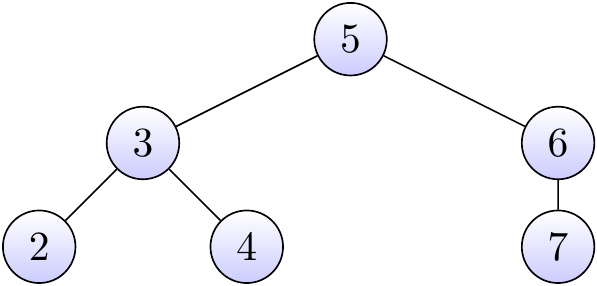
\includegraphics[width=0.9\linewidth]{bookdown-demo_files/figure-latex/unnamed-chunk-1-1} \caption{Some caption.}\label{fig:unnamed-chunk-1}
\end{figure}

Target = 9, Output = True.

\hypertarget{solution-1}{%
\subsection{Solution}\label{solution-1}}

\hypertarget{walkthrough-3}{%
\subsubsection{Walkthrough}\label{walkthrough-3}}

Use a HashSet to store value of current node, that is (node.val). Then check if answer = (target - node.val)
and return true if existed; otherwise, recursively call the same function for its left and right children.

\hypertarget{analysis-3}{%
\subsubsection{Analysis}\label{analysis-3}}

Time complexity is O(n) since every node is visited. Auxiliary Space is O(1)

\hypertarget{algorithm-3}{%
\subsubsection{Algorithm}\label{algorithm-3}}

\{recursive\}

\hypertarget{java-code-1}{%
\subsection{Java Code}\label{java-code-1}}

\begin{Shaded}
\begin{Highlighting}[]
\KeywordTok{public} \DataTypeTok{boolean} \FunctionTok{findTarget}\NormalTok{(}\BuiltInTok{TreeNode}\NormalTok{ root, }\DataTypeTok{int}\NormalTok{ target) \{}
    \BuiltInTok{Set}\NormalTok{<}\BuiltInTok{Integer}\NormalTok{> set = }\KeywordTok{new} \BuiltInTok{HashSet}\NormalTok{<>();}
    \KeywordTok{return} \FunctionTok{findTarget}\NormalTok{(root, target, set);}
\NormalTok{\}}

\KeywordTok{public} \DataTypeTok{boolean} \FunctionTok{findTarget}\NormalTok{(}\BuiltInTok{TreeNode}\NormalTok{ node, }\DataTypeTok{int}\NormalTok{ target, }\BuiltInTok{Set}\NormalTok{<}\BuiltInTok{Integer}\NormalTok{> set) \{}
    \KeywordTok{if}\NormalTok{(node == }\KeywordTok{null}\NormalTok{) \{}
        \KeywordTok{return} \KeywordTok{false}\NormalTok{;}
\NormalTok{    \} }\KeywordTok{else} \KeywordTok{if}\NormalTok{(set.}\FunctionTok{contains}\NormalTok{(target - node.}\FunctionTok{val}\NormalTok{)) \{}
        \KeywordTok{return} \KeywordTok{true}\NormalTok{;}
\NormalTok{    \} }\KeywordTok{else}\NormalTok{ \{}
        \CommentTok{//recursively calling}
\NormalTok{        set.}\FunctionTok{add}\NormalTok{(node.}\FunctionTok{val}\NormalTok{);}
        \KeywordTok{return} \FunctionTok{findTarget}\NormalTok{(node.}\FunctionTok{right}\NormalTok{, target, set) || }\FunctionTok{findTarget}\NormalTok{(node.}\FunctionTok{left}\NormalTok{, target, set);}
\NormalTok{    \}}

\NormalTok{\}}
\end{Highlighting}
\end{Shaded}

\hypertarget{twosum-v}{%
\section{TwoSum V / / \}}\label{twosum-v}}

\hypertarget{description-3}{%
\subsection{Description}\label{description-3}}

Given a sorted array S of n integers, are there elements a, b in S such that a + b = target? Find all unique
pairs in the array which gives the sum of zero. Note: The solution set must not contain duplicate triplets.

\hypertarget{example-2}{%
\subsection{Example}\label{example-2}}

For example, given array S = {[}-2, -1, -1, 0, 1, 2{]}, target = 0
A solution set is:
{[}
{[}-1, 1{]},
{[}-2, 2{]}{]}

\hypertarget{solution-2}{%
\subsection{Solution}\label{solution-2}}

\hypertarget{walkthrough-4}{%
\subsubsection{Walkthrough}\label{walkthrough-4}}

While searching for the other two elements from both ends, with indices left incrementally and right decrmentally, find
the sum = nums{[}left{]} + nums{[}right{]} == target. Since the array is
sorted, we need to avoid duplicated entry by moving forward the index while searching.

\hypertarget{analysis-4}{%
\subsubsection{Analysis}\label{analysis-4}}

There are one loops, the time complexity is \(O(n)\), and Auxiliary Space is \(O(n)\) since one member of any pair is
uniquely determined by the other member. If the numbers are not distinct, the Auxiliary Space as large as
\(O(\binom{n}{2}) = O(\frac{n!}{2!\cdot (n-2)!}) = O(\frac{n\cdot (n-1)}{2}) = O(n^2)\)

\hypertarget{algorithm-4}{%
\subsubsection{Algorithm}\label{algorithm-4}}

\hypertarget{java-code-2}{%
\subsection{Java Code}\label{java-code-2}}

\begin{Shaded}
\begin{Highlighting}[]
\KeywordTok{public} \BuiltInTok{List}\NormalTok{<}\BuiltInTok{List}\NormalTok{<}\BuiltInTok{Integer}\NormalTok{>> }\FunctionTok{twoSum}\NormalTok{(}\DataTypeTok{int}\NormalTok{[] num, }\DataTypeTok{int}\NormalTok{ target) \{}
    \BuiltInTok{List}\NormalTok{<}\BuiltInTok{List}\NormalTok{<}\BuiltInTok{Integer}\NormalTok{>> result = }\KeywordTok{new} \BuiltInTok{ArrayList}\NormalTok{<>();}

    \DataTypeTok{int}\NormalTok{ left = }\DecValTok{0}\NormalTok{, right = num.}\FunctionTok{length}\NormalTok{ - }\DecValTok{1}\NormalTok{;}

    \KeywordTok{while}\NormalTok{ (left < right) \{}
        \DataTypeTok{int}\NormalTok{ sum = num[left] + num[right];}

        \KeywordTok{if}\NormalTok{ (sum == target) \{}
\NormalTok{            result.}\FunctionTok{add}\NormalTok{(}\BuiltInTok{Arrays}\NormalTok{.}\FunctionTok{asList}\NormalTok{(num[left], num[right]));}

            \CommentTok{//avoid duplicated entry by moving forward the index}
            \KeywordTok{while}\NormalTok{ (left < right && num[left] == num[left + }\DecValTok{1}\NormalTok{]) \{}
\NormalTok{                left++;}
\NormalTok{            \}}
            \KeywordTok{while}\NormalTok{ (left < right && num[right] == num[right - }\DecValTok{1}\NormalTok{]) \{}
\NormalTok{                right--;}
\NormalTok{            \}}

\NormalTok{            left++;}
\NormalTok{            right--;}
\NormalTok{        \} }\KeywordTok{else} \KeywordTok{if}\NormalTok{ (sum < target) \{}
\NormalTok{            left++;}
\NormalTok{        \} }\KeywordTok{else}\NormalTok{ \{}
            \CommentTok{// sum > target}
\NormalTok{            right--;}
\NormalTok{        \}}
\NormalTok{    \}}

    \KeywordTok{return}\NormalTok{ result;}
\NormalTok{\}}
\end{Highlighting}
\end{Shaded}

\hypertarget{sum-leet-code-15-medium}{%
\section{3Sum / Leet Code 15 / Medium\}}\label{sum-leet-code-15-medium}}

\hypertarget{description-4}{%
\subsection{Description}\label{description-4}}

Given an array S of n integers, are there elements a, b, c in S such that a + b + c = 0? Find all unique triplets in the array which
gives the sum of zero. Note: The solution set must not contain duplicate triplets.

\hypertarget{example-3}{%
\subsection{Example}\label{example-3}}

For example, given array S = {[}-1, 0, 1, 2, -1, -4{]},
A solution set is:
{[}
{[}-1, 0, 1{]},
{[}-1, -1, 2{]}{]}

\hypertarget{solution-3}{%
\subsection{Solution}\label{solution-3}}

\hypertarget{walkthrough-5}{%
\subsubsection{Walkthrough}\label{walkthrough-5}}

Looping the array with index i, while searching for the other two elements from both ends, with indices
left incrementally and right decrmentally, find the sum = nums{[}i{]} + nums{[}left{]} + nums{[}right{]} == 0. Since the array is
sorted, we need to avoid duplicated entry by moving forward the index while searching.

\hypertarget{analysis-5}{%
\subsubsection{Analysis}\label{analysis-5}}

There are two nested loops, the time complexity is \(O(n^2)\), and Auxiliary Space is is \(O(n^2)\) since one member of any
triplet is uniquely determined by the other two members. If the numbers are not distinct, the Auxiliary Space as large as
\(O(\binom{n}{3}) = O(\frac{n!}{3!\cdot (n-3)!}) = O(\frac{n\cdot (n-1)\cdot(n-2)}{3}) = O(n^3)\)

\hypertarget{algorithm-5}{%
\subsubsection{Algorithm}\label{algorithm-5}}

\hypertarget{java-code-3}{%
\subsection{Java Code}\label{java-code-3}}

\begin{Shaded}
\begin{Highlighting}[]
\KeywordTok{public} \BuiltInTok{List}\NormalTok{<}\BuiltInTok{List}\NormalTok{<}\BuiltInTok{Integer}\NormalTok{>> }\FunctionTok{threeSum}\NormalTok{(}\DataTypeTok{int}\NormalTok{[] num) \{}
    \BuiltInTok{Arrays}\NormalTok{.}\FunctionTok{sort}\NormalTok{(num); }\CommentTok{//sort}
    \BuiltInTok{List}\NormalTok{<}\BuiltInTok{List}\NormalTok{<}\BuiltInTok{Integer}\NormalTok{>> result = }\KeywordTok{new} \BuiltInTok{ArrayList}\NormalTok{<>();}

    \CommentTok{//last possible pair is [i=len - 3, left=len - 2, right=len - 1]}
    \KeywordTok{for}\NormalTok{ (}\DataTypeTok{int}\NormalTok{ i = }\DecValTok{0}\NormalTok{; i < num.}\FunctionTok{length}\NormalTok{ - }\DecValTok{2}\NormalTok{; i++) \{}
        \CommentTok{// Since the array is sorted, we need to avoid duplicated entry by moving forward the index}
        \KeywordTok{if}\NormalTok{ (i == }\DecValTok{0}\NormalTok{ || (i > }\DecValTok{0}\NormalTok{ && num[i] != num[i}\DecValTok{-1}\NormalTok{])) \{}
            \DataTypeTok{int}\NormalTok{ left = i + }\DecValTok{1}\NormalTok{, right = num.}\FunctionTok{length}\DecValTok{-1}\NormalTok{;}

            \KeywordTok{while}\NormalTok{ (left < right) \{}
                \DataTypeTok{int}\NormalTok{ sum = num[i] + num[left] + num[right];}

                \KeywordTok{if}\NormalTok{ (sum == }\DecValTok{0}\NormalTok{) \{}
\NormalTok{                    result.}\FunctionTok{add}\NormalTok{(}\BuiltInTok{Arrays}\NormalTok{.}\FunctionTok{asList}\NormalTok{(num[i], num[left], num[right]));}

                    \CommentTok{//avoid duplicated entry by moving forward the index}
                    \KeywordTok{while}\NormalTok{ (left < right && num[left] == num[left + }\DecValTok{1}\NormalTok{]) \{}
\NormalTok{                        left++;}
\NormalTok{                    \}}
                    \KeywordTok{while}\NormalTok{ (left < right && num[right] == num[right - }\DecValTok{1}\NormalTok{]) \{}
\NormalTok{                        right--;}
\NormalTok{                    \}}

\NormalTok{                    left++;}
\NormalTok{                    right--;}
\NormalTok{                \} }\KeywordTok{else} \KeywordTok{if}\NormalTok{ (sum < }\DecValTok{0}\NormalTok{) \{}
\NormalTok{                    left++;}
\NormalTok{                \} }\KeywordTok{else}\NormalTok{ \{}
                    \CommentTok{// sum > 0}
\NormalTok{                    right--;}
\NormalTok{                \}}
\NormalTok{            \}}
\NormalTok{        \}}
\NormalTok{    \}}

    \KeywordTok{return}\NormalTok{ result;}
\NormalTok{\}}
\end{Highlighting}
\end{Shaded}

\hypertarget{sum-closest-leetcode-16-medium}{%
\section{3 Sum Closest / LeetCode 16 / Medium\}}\label{sum-closest-leetcode-16-medium}}

\hypertarget{description-5}{%
\subsection{Description}\label{description-5}}

Given an array S of n integers, find three integers in S such that the sum is closest to a given number, target.
Return the sum of the three integers. You may assume that each input would have exactly one solution.

\hypertarget{example-4}{%
\subsection{Example}\label{example-4}}

For example, given array S = -1 2 1 -4, and target = 1.
The sum that is closest to the target is 2. (-1 + 2 + 1 = 2).

\hypertarget{solution-4}{%
\subsection{Solution}\label{solution-4}}

\hypertarget{walkthrough-6}{%
\subsubsection{Walkthrough}\label{walkthrough-6}}

Looping the array with index i, while searching for the other two elements from both ends, with indices
left incrementally and right decrmentally, find the sum = nums{[}i{]} + nums{[}left{]} + nums{[}right{]}. Return sum if existed;
otherwise, keep for the closest tuple of (nums{[}i{]}, nums{[}left{]}, nums{[}right{]}) against target using Math.abs().

\hypertarget{analysis-6}{%
\subsubsection{Analysis}\label{analysis-6}}

There are two nested loops, the time complexity is \(O(n^2)\), and Auxiliary Space is O(1) since it is returning the closest answer.

\hypertarget{algorithm-6}{%
\subsubsection{Algorithm}\label{algorithm-6}}

\hypertarget{java-code-4}{%
\subsection{Java Code}\label{java-code-4}}

\begin{Shaded}
\begin{Highlighting}[]
\KeywordTok{public} \DataTypeTok{int} \FunctionTok{threeSumClosest}\NormalTok{(}\DataTypeTok{int}\NormalTok{[] nums, }\DataTypeTok{int}\NormalTok{ target) \{}
    \BuiltInTok{Arrays}\NormalTok{.}\FunctionTok{sort}\NormalTok{(num); }\CommentTok{//sort}
    \DataTypeTok{int}\NormalTok{ minDelta = }\BuiltInTok{Integer}\NormalTok{.}\FunctionTok{MAX_VALUE}\NormalTok{, result = }\DecValTok{0}\NormalTok{;}

    \CommentTok{//last possible pair is [i=len - 3, left=len - 2, right=len - 1]}
    \KeywordTok{for}\NormalTok{ (}\DataTypeTok{int}\NormalTok{ i = }\DecValTok{0}\NormalTok{; i < num.}\FunctionTok{length}\NormalTok{ - }\DecValTok{2}\NormalTok{; i++) \{}
        \DataTypeTok{int}\NormalTok{ left = i + }\DecValTok{1}\NormalTok{, right = num.}\FunctionTok{length}\NormalTok{ - }\DecValTok{1}\NormalTok{;}

        \KeywordTok{while}\NormalTok{ (left < right) \{}
            \DataTypeTok{int}\NormalTok{ sum = num[i] + num[left] + num[right];}

            \KeywordTok{if}\NormalTok{ (sum == target) \{}
                \CommentTok{//find exact match}
                \KeywordTok{return}\NormalTok{ sum;}
\NormalTok{            \} }\KeywordTok{else} \KeywordTok{if}\NormalTok{ (sum < target) \{}
\NormalTok{                left++;}
\NormalTok{            \} }\KeywordTok{else}\NormalTok{ \{}
                \CommentTok{// sum > target}
\NormalTok{                right--;}
\NormalTok{            \}}

            \DataTypeTok{int}\NormalTok{ delta = }\BuiltInTok{Math}\NormalTok{.}\FunctionTok{abs}\NormalTok{(sum - target);}
            \KeywordTok{if}\NormalTok{(delta < minDelta) \{}
\NormalTok{                minDelta = delta;}
\NormalTok{                result = sum;}
\NormalTok{            \}}
\NormalTok{        \}}
\NormalTok{    \}}

    \KeywordTok{return}\NormalTok{ result;}
\NormalTok{\}}
\end{Highlighting}
\end{Shaded}

\hypertarget{sum-leet-code-18-medium}{%
\section{4Sum / Leet Code 18 / Medium\}}\label{sum-leet-code-18-medium}}

\hypertarget{description-6}{%
\subsection{Description}\label{description-6}}

Given an array nums of n integers and an integer target, are there elements a, b, c, and d in nums such that
a + b + c + d = target? Find all unique quadruplets in the array which gives the sum of target. The solution set
must not contain duplicate quadruplets.

\hypertarget{example-5}{%
\subsection{Example}\label{example-5}}

Given array nums = {[}1, 0, -1, 0, -2, 2{]}, and target = 0.

A solution set is:
{[}
{[}-1, 0, 0, 1{]},
{[}-2, -1, 1, 2{]},
{[}-2, 0, 0, 2{]}{]}

\hypertarget{solution-5}{%
\subsection{Solution}\label{solution-5}}

\hypertarget{walkthrough-7}{%
\subsubsection{Walkthrough}\label{walkthrough-7}}

The solution is similar to 3Sum to find the sum = nums{[}i{]} + nums{[}j{]} + nums{[}left{]} + nums{[}right{]} == target. The only
difference is there is an extra loop as well as we need to avoid duplicated entry by moving forward the index
during search.

\hypertarget{analysis-7}{%
\subsubsection{Analysis}\label{analysis-7}}

Overall, there are three nested loops, the time complexity is \(O(n^3)\), and Auxiliary Space is \(O(n^3)\) since one member
of any quotriplet is uniquely determined by the other three member. If the numbers are not distinct, the Auxiliary
Space as large as is \(O(\binom{n}{4}) = O(n^4)\)

\hypertarget{algorithm-7}{%
\subsubsection{Algorithm}\label{algorithm-7}}

\hypertarget{java-code-5}{%
\subsection{Java Code}\label{java-code-5}}

\begin{Shaded}
\begin{Highlighting}[]
\KeywordTok{public} \BuiltInTok{List}\NormalTok{<}\BuiltInTok{List}\NormalTok{<}\BuiltInTok{Integer}\NormalTok{>> }\FunctionTok{fourSum}\NormalTok{(}\DataTypeTok{int}\NormalTok{[] num, }\DataTypeTok{int}\NormalTok{ target) \{}
    \BuiltInTok{Arrays}\NormalTok{.}\FunctionTok{sort}\NormalTok{(num); }\CommentTok{//sort}
    \BuiltInTok{List}\NormalTok{<}\BuiltInTok{List}\NormalTok{<}\BuiltInTok{Integer}\NormalTok{>> res = }\KeywordTok{new} \BuiltInTok{LinkedList}\NormalTok{<>();}

    \CommentTok{//last possible pair is [j=len - 4, i=len-3, left=len - 2, right=len - 1]}
    \KeywordTok{for}\NormalTok{ (}\DataTypeTok{int}\NormalTok{ j = }\DecValTok{0}\NormalTok{; i < num.}\FunctionTok{length}\NormalTok{ - }\DecValTok{3}\NormalTok{; i++) \{}

        \CommentTok{// Since the array is sorted, we need to avoid duplicated entry by moving forward the index}
        \KeywordTok{if}\NormalTok{ (j == }\DecValTok{0}\NormalTok{ || (j > }\DecValTok{0}\NormalTok{ && num[j] != num[j - }\DecValTok{1}\NormalTok{])) \{}
            \KeywordTok{for}\NormalTok{ (}\DataTypeTok{int}\NormalTok{ i = j + }\DecValTok{1}\NormalTok{; i < num.}\FunctionTok{length}\NormalTok{ - }\DecValTok{2}\NormalTok{; i++) \{}

                \CommentTok{// Since the array is sorted, we need to avoid duplicated entry by moving forward the index}
                \KeywordTok{if}\NormalTok{ (i == j + }\DecValTok{1}\NormalTok{ || (i > }\DecValTok{0}\NormalTok{ && num[i] != num[i - }\DecValTok{1}\NormalTok{])) \{}
                    \DataTypeTok{int}\NormalTok{ left = i + }\DecValTok{1}\NormalTok{, right = num.}\FunctionTok{length}\DecValTok{-1}\NormalTok{;}

                    \KeywordTok{while}\NormalTok{ (left < right) \{}
                        \DataTypeTok{int}\NormalTok{ sum = num[i] + num[j] + num[left] + num[right];}

                        \KeywordTok{if}\NormalTok{ (sum == target) \{}
\NormalTok{                            res.}\FunctionTok{add}\NormalTok{(}\BuiltInTok{Arrays}\NormalTok{.}\FunctionTok{asList}\NormalTok{(num[i], num[j], num[left], num[right]));}

                            \CommentTok{//avoid duplicated entry by moving forward the index}
                            \KeywordTok{while}\NormalTok{ (left < right && num[left] == num[left + }\DecValTok{1}\NormalTok{]) \{}
\NormalTok{                                left++;}
\NormalTok{                            \}}
                            \KeywordTok{while}\NormalTok{ (left < right && num[right] == num[right - }\DecValTok{1}\NormalTok{]) \{}
\NormalTok{                                right--;}
\NormalTok{                            \}}
\NormalTok{                            left++;}
\NormalTok{                            right--;}
\NormalTok{                        \} }\KeywordTok{else} \KeywordTok{if}\NormalTok{ (sum < target) \{}
\NormalTok{                            left++;}
\NormalTok{                        \} }\KeywordTok{else}\NormalTok{ \{}
                            \CommentTok{// sum > 0}
\NormalTok{                            right--;}
\NormalTok{                        \}}
\NormalTok{                    \}}
\NormalTok{                \}}
\NormalTok{            \}}
\NormalTok{        \}}
\NormalTok{    \}}

    \KeywordTok{return}\NormalTok{ res;}
\NormalTok{\}}
\end{Highlighting}
\end{Shaded}

\hypertarget{sum-ii}{%
\section{4Sum II\}}\label{sum-ii}}

\hypertarget{description-7}{%
\subsection{Description}\label{description-7}}

Given four lists A, B, C, D of integer values, compute how many tuples (i, j, k, l) there are such that
A{[}i{]} + B{[}j{]} + C{[}k{]} + D{[}l{]} is zero.

To make problem a bit easier, all A, B, C, D have same length of N where \(0 \le N \le 500\). All integers are
in the range of \(-2^{28}\) to \(2^{28} - 1\) and the result is guaranteed to be at most \(2^{31} - 1\).

\hypertarget{example-6}{%
\subsection{Example}\label{example-6}}

Input:
A = {[} 1, 2{]}
B = {[}-2,-1{]}
C = {[}-1, 2{]}
D = {[} 0, 2{]}

Output:
2

Explanation:
The two tuples are:
1. (0, 0, 0, 1) \(->\) A{[}0{]} + B{[}0{]} + C{[}0{]} + D{[}1{]} = 1 + (-2) + (-1) + 2 = 0
2. (1, 1, 0, 0) \(->\) A{[}1{]} + B{[}1{]} + C{[}0{]} + D{[}0{]} = 2 + (-1) + (-1) + 0 = 0
\#\#\# Solution
\#\#\#\# Walkthrough
*Rewrite the equation as A{[}i{]} + B{[}j{]} = -(C{[}k{]} + D{[}l{]}).
Create a Map\textless{}Integer, Integer\textgreater{} where `key' is A{[}i{]} + B{[}j{]} and `value' is the number of pairs with this sum.
For each -(C{[}k{]} + D{[}l{]}), see if this desired sum is in our map. If so, add the map's `value' to our total count.

\hypertarget{analysis-8}{%
\subsubsection{Analysis}\label{analysis-8}}

There are two nested loops, the time complexity is \(O(n^2)\), and Auxiliary Space for Map is O(n)

\hypertarget{algorithm-8}{%
\subsubsection{Algorithm}\label{algorithm-8}}

\hypertarget{java-code-6}{%
\subsection{Java Code}\label{java-code-6}}

\begin{Shaded}
\begin{Highlighting}[]
\KeywordTok{public} \DataTypeTok{int} \FunctionTok{fourSumCount}\NormalTok{(}\DataTypeTok{int}\NormalTok{[] A, }\DataTypeTok{int}\NormalTok{[] B, }\DataTypeTok{int}\NormalTok{[] C, }\DataTypeTok{int}\NormalTok{[] D) \{}
    \DataTypeTok{int}\NormalTok{ n = A.}\FunctionTok{length}\NormalTok{;}

    \KeywordTok{if}\NormalTok{(n == }\DecValTok{0}\NormalTok{) \{}
        \KeywordTok{return} \DecValTok{0}\NormalTok{;}
\NormalTok{    \}}

    \DataTypeTok{int}\NormalTok{[] sumOfAandB = }\KeywordTok{new} \DataTypeTok{int}\NormalTok{[n * n];}
    \DataTypeTok{int}\NormalTok{ result = }\DecValTok{0}\NormalTok{;}

    \BuiltInTok{HashMap}\NormalTok{<}\BuiltInTok{Integer}\NormalTok{, }\BuiltInTok{Integer}\NormalTok{> map = }\KeywordTok{new} \BuiltInTok{HashMap}\NormalTok{<}\BuiltInTok{Integer}\NormalTok{, }\BuiltInTok{Integer}\NormalTok{>();}

    \KeywordTok{for}\NormalTok{(}\DataTypeTok{int}\NormalTok{ i = }\DecValTok{0}\NormalTok{; i < n; i++)\{}
        \KeywordTok{for}\NormalTok{(}\DataTypeTok{int}\NormalTok{ j = }\DecValTok{0}\NormalTok{; j < n; j++)\{}
\NormalTok{            sumOfAandB[i*n + j] = A[i] + B[j];}

            \CommentTok{//record # of pairs for this sum of [A, B]}
            \DataTypeTok{int}\NormalTok{ count = map.}\FunctionTok{getOrDefault}\NormalTok{(sumOfAandB[i*n + j], }\DecValTok{0}\NormalTok{) + }\DecValTok{1}\NormalTok{;}
\NormalTok{            map.}\FunctionTok{put}\NormalTok{(sumOfAandB[i*n + j], count);}
\NormalTok{        \}}
\NormalTok{    \}}

    \CommentTok{//A + B = - (C + D)}
    \KeywordTok{for}\NormalTok{(}\DataTypeTok{int}\NormalTok{ i = }\DecValTok{0}\NormalTok{; i < n; i++)\{}
        \KeywordTok{for}\NormalTok{(}\DataTypeTok{int}\NormalTok{ j = }\DecValTok{0}\NormalTok{; j < n; j++)\{}
            \DataTypeTok{int}\NormalTok{ sumOfCandD = - (C[i] + D[j]);}

            \KeywordTok{if}\NormalTok{(map.}\FunctionTok{containsKey}\NormalTok{(sumOfCandD))\{}
\NormalTok{                result += map.}\FunctionTok{get}\NormalTok{(sumOfCandD);}
\NormalTok{            \}}
\NormalTok{        \}}
\NormalTok{    \}}


    \KeywordTok{return}\NormalTok{ result;}
\NormalTok{\}}
\end{Highlighting}
\end{Shaded}

\hypertarget{max-gain-firecode-level-2}{%
\section{Max Gain / Firecode / Level 2\}}\label{max-gain-firecode-level-2}}

\hypertarget{description-8}{%
\subsection{Description}\label{description-8}}

Given an array of integers, write a method - maxGain - that returns the maximum gain. Maximum Gain is defined as the
maximum difference between 2 elements in a list such that the larger element appears after the smaller element. If no
gain is possible, return 0.

\hypertarget{example-7}{%
\subsection{Example}\label{example-7}}

{[}0,50,10,100,30{]} returns 100

{[}100,40,20,10{]} returns 0

{[}0,100,0,100,0,100{]} returns 100

\hypertarget{solution-6}{%
\subsection{Solution}\label{solution-6}}

\hypertarget{walkthrough-8}{%
\subsubsection{Walkthrough}\label{walkthrough-8}}

By definition, \textbf{the larger element must always appear after the smaller element}, we could do this in one pass
by finding the minimum element and the maximum gain (so far) by Math.max(min, a{[}i{]} - min)

\hypertarget{analysis-9}{%
\subsubsection{Analysis}\label{analysis-9}}

The time complexity is O(n) since every element is visited in the loop.

\hypertarget{algorithm-9}{%
\subsubsection{Algorithm}\label{algorithm-9}}

\hypertarget{java-code-7}{%
\subsection{Java Code}\label{java-code-7}}

\begin{Shaded}
\begin{Highlighting}[]
\KeywordTok{public} \DataTypeTok{static} \DataTypeTok{int} \FunctionTok{maxGain}\NormalTok{(}\DataTypeTok{int}\NormalTok{[] a) \{}
    \DataTypeTok{int}\NormalTok{ min = }\BuiltInTok{Integer}\NormalTok{.}\FunctionTok{MAX_VALUE}\NormalTok{, gain = }\DecValTok{0}\NormalTok{;}

    \KeywordTok{for}\NormalTok{(}\DataTypeTok{int}\NormalTok{ i = }\DecValTok{0}\NormalTok{; i < a.}\FunctionTok{length}\NormalTok{; i++) \{}
\NormalTok{        min = }\BuiltInTok{Math}\NormalTok{.}\FunctionTok{min}\NormalTok{(min, a[i]);}
\NormalTok{        gain = }\BuiltInTok{Math}\NormalTok{.}\FunctionTok{max}\NormalTok{(gain, a[i] - min);}
\NormalTok{    \}}

    \KeywordTok{return}\NormalTok{ gain;}
\NormalTok{\}}
\end{Highlighting}
\end{Shaded}

\hypertarget{pascals-triangle-leet-code-118-easy}{%
\section{Pascal's Triangle / Leet Code 118 / Easy\}}\label{pascals-triangle-leet-code-118-easy}}

\hypertarget{description-9}{%
\subsection{Description}\label{description-9}}

Given a non-negative integer numRows, generate the first numRows of Pascal's triangle. In Pascal's triangle, each
number is the sum of the two numbers directly above it.

\hypertarget{example-8}{%
\subsection{Example}\label{example-8}}

\hypertarget{solution-7}{%
\subsection{Solution}\label{solution-7}}

\hypertarget{walkthrough-9}{%
\subsubsection{Walkthrough}\label{walkthrough-9}}

For level 1 and level 2, add number 1. For level 3 or above if it is the first or last element, insert 1, otherwise,
insert the sum of last two elements in the level above : {[}i-1{]}{[}j{]} + {[}i-1{]}{[}j-1{]}.

\hypertarget{analysis-10}{%
\subsubsection{Analysis}\label{analysis-10}}

There are two nested loops, the time complexity is \(O(n^2)\)\$, and Auxiliary Space is \(O(n^2)\).

\hypertarget{algorithm-10}{%
\subsubsection{Algorithm}\label{algorithm-10}}

\hypertarget{java-code-8}{%
\subsection{Java Code}\label{java-code-8}}

\begin{Shaded}
\begin{Highlighting}[]
\KeywordTok{public} \BuiltInTok{List}\NormalTok{<}\BuiltInTok{List}\NormalTok{<}\BuiltInTok{Integer}\NormalTok{>> }\FunctionTok{generate}\NormalTok{(}\DataTypeTok{int}\NormalTok{ numRows) \{}
    \BuiltInTok{List}\NormalTok{<}\BuiltInTok{List}\NormalTok{<}\BuiltInTok{Integer}\NormalTok{>> triangle = }\KeywordTok{new} \BuiltInTok{ArrayList}\NormalTok{<>();}

    \KeywordTok{for}\NormalTok{(}\DataTypeTok{int}\NormalTok{ i = }\DecValTok{0}\NormalTok{; i < numRows; i++) \{}
        \BuiltInTok{List}\NormalTok{<}\BuiltInTok{Integer}\NormalTok{> level = }\KeywordTok{new} \BuiltInTok{ArrayList}\NormalTok{<>();}

        \KeywordTok{for}\NormalTok{(}\DataTypeTok{int}\NormalTok{ j = }\DecValTok{0}\NormalTok{; j < (i+}\DecValTok{1}\NormalTok{); j++) \{}
            \KeywordTok{if}\NormalTok{(i == }\DecValTok{0}\NormalTok{ || i == }\DecValTok{1}\NormalTok{) \{}
                \CommentTok{// for level 1 or level 2}
\NormalTok{                level.}\FunctionTok{add}\NormalTok{(}\DecValTok{1}\NormalTok{);}
\NormalTok{            \} }\KeywordTok{else}\NormalTok{ \{}
                \CommentTok{// for level 3 or above}
                \KeywordTok{if}\NormalTok{(j == }\DecValTok{0}\NormalTok{ || j == i) \{}
\NormalTok{                    level.}\FunctionTok{add}\NormalTok{(}\DecValTok{1}\NormalTok{);}
\NormalTok{                \} }\KeywordTok{else}\NormalTok{ \{}
                    \DataTypeTok{int}\NormalTok{ op1 = triangle.}\FunctionTok{get}\NormalTok{(i}\DecValTok{-1}\NormalTok{).}\FunctionTok{get}\NormalTok{(j}\DecValTok{-1}\NormalTok{);}
                    \DataTypeTok{int}\NormalTok{ op2 = triangle.}\FunctionTok{get}\NormalTok{(i}\DecValTok{-1}\NormalTok{).}\FunctionTok{get}\NormalTok{(j);}
\NormalTok{                    level.}\FunctionTok{add}\NormalTok{(op1 + op2);}
\NormalTok{                \}}
\NormalTok{            \}}
\NormalTok{        \}}

\NormalTok{        triangle.}\FunctionTok{add}\NormalTok{(level);}
\NormalTok{    \}}

    \KeywordTok{return}\NormalTok{ triangle;}
\NormalTok{\}}
\end{Highlighting}
\end{Shaded}

\hypertarget{search-in-rotated-sorted-array-leet-code-33-medium}{%
\section{Search in Rotated Sorted Array / Leet Code 33 / Medium \}}\label{search-in-rotated-sorted-array-leet-code-33-medium}}

\hypertarget{description-10}{%
\subsection{Description}\label{description-10}}

Suppose an array sorted in ascending order is rotated at some pivot unknown to you beforehand.
(i.e., {[}0,1,2,4,5,6,7{]} might become {[}4,5,6,7,0,1,2{]}).

You are given a target value to search. If found in the array return its index, otherwise return -1. You may
assume no duplicate exists in the array. Your algorithm's runtime complexity must be in the order of O(log n).

\hypertarget{example-9}{%
\subsection{Example}\label{example-9}}

Input: nums = {[}4,5,6,7,0,1,2{]}, target = 0
Output: 4

Input: nums = {[}4,5,6,7,0,1,2{]}, target = 3
Output: -1
\#\#\# Solution
\#\#\#\# Walkthrough
The key point is to search the element in a divide-and-conquer manner. We need to repeated compare the
mid element of index = (left + right) / 2 with target and keep shrinking the boundaries from left and right two ends
according to the conditions. Return the mid index if found; otherwise, return -1.

\hypertarget{analysis-11}{%
\subsubsection{Analysis}\label{analysis-11}}

The time complexity is O(log n) since we only pick one from half of target elements each time.

\hypertarget{algorithm-11}{%
\subsubsection{Algorithm}\label{algorithm-11}}

\{dnc\}

\hypertarget{java-code-9}{%
\subsection{Java Code}\label{java-code-9}}

\begin{Shaded}
\begin{Highlighting}[]
\KeywordTok{public} \DataTypeTok{int} \FunctionTok{search}\NormalTok{(}\DataTypeTok{int}\NormalTok{[] nums, }\DataTypeTok{int}\NormalTok{ target) \{}
    \DataTypeTok{int}\NormalTok{ left = }\DecValTok{0}\NormalTok{, right = nums.}\FunctionTok{length}\NormalTok{ - }\DecValTok{1}\NormalTok{;}

    \KeywordTok{while}\NormalTok{(left <= right) \{}
        \DataTypeTok{int}\NormalTok{ mid = (right - left) / }\DecValTok{2}\NormalTok{ + left;}

        \KeywordTok{if}\NormalTok{(nums[mid] == target) \{}
            \CommentTok{//Found index}
            \KeywordTok{return}\NormalTok{ mid;}
\NormalTok{        \} }\KeywordTok{else} \KeywordTok{if}\NormalTok{(nums[mid] >= nums[left]) \{}
            \CommentTok{//left half of array}
            \KeywordTok{if}\NormalTok{(target >= nums[left] && target < nums[mid]) \{}
                \CommentTok{//<-- moving leftward}
\NormalTok{                right = mid }\DecValTok{-1}\NormalTok{;}
\NormalTok{            \} }\KeywordTok{else}\NormalTok{ \{}
                \CommentTok{//--> moving rightward}
\NormalTok{                left = mid + }\DecValTok{1}\NormalTok{;}
\NormalTok{            \}}
\NormalTok{        \} }\KeywordTok{else}\NormalTok{ \{}
            \CommentTok{//nums[mid] < nums[right}
            \CommentTok{//right half of array}
            \KeywordTok{if}\NormalTok{(target > nums[mid] && target <= nums[right]) \{}
                \CommentTok{//--> moving rightward}
\NormalTok{                left = mid + }\DecValTok{1}\NormalTok{;}
\NormalTok{            \} }\KeywordTok{else}\NormalTok{ \{}
                \CommentTok{//<-- moving leftward}
\NormalTok{                right = mid - }\DecValTok{1}\NormalTok{;}
\NormalTok{            \}}
\NormalTok{        \}}
\NormalTok{    \}}

    \KeywordTok{return} \DecValTok{-1}\NormalTok{;}
\NormalTok{\}}
\end{Highlighting}
\end{Shaded}

\hypertarget{median-of-two-sorted-arrays-leet-code-4-hard}{%
\section{Median of Two Sorted Arrays / Leet Code 4 / Hard\}}\label{median-of-two-sorted-arrays-leet-code-4-hard}}

\hypertarget{description-11}{%
\subsection{Description}\label{description-11}}

There are two sorted arrays nums1 and nums2 of size m and n respectively. Find the median of the two sorted
arrays. The overall run time complexity should be O(log (m+n)). You may assume nums1 and nums2 cannot be both
empty.

\hypertarget{example-10}{%
\subsection{Example}\label{example-10}}

nums1 = {[}1, 3{]}, nums2 = {[}2{]}, The median is 2.0

nums1 = {[}1, 2{]}, nums2 = {[}3, 4{]}, The median is (2 + 3)/2 = 2.5

\hypertarget{solution-8}{%
\subsection{Solution}\label{solution-8}}

\hypertarget{walkthrough-10}{%
\subsubsection{Walkthrough}\label{walkthrough-10}}

Recursively find \(K^{th}\) element in two sorted array by comparing and discarding the \(\frac{k}{2}\) smaller
elements.

\hypertarget{analysis-12}{%
\subsubsection{Analysis}\label{analysis-12}}

For each round of recursive, it is eliminating \(\frac{k}{2}\) element, so total time complexity is
\(O(log(k)) = O(log(m + n))\). Auxiliary Space is O(1).

\hypertarget{algorithm-12}{%
\subsubsection{Algorithm}\label{algorithm-12}}

\{recursive\}

\hypertarget{java-code-10}{%
\subsection{Java Code}\label{java-code-10}}

\begin{Shaded}
\begin{Highlighting}[]
\KeywordTok{public} \DataTypeTok{double} \FunctionTok{findMedianSortedArrays}\NormalTok{(}\DataTypeTok{int}\NormalTok{[] nums1, }\DataTypeTok{int}\NormalTok{[] nums2) \{}
    \DataTypeTok{int}\NormalTok{ len1 = nums1.}\FunctionTok{length}\NormalTok{;}
    \DataTypeTok{int}\NormalTok{ len2 = nums2.}\FunctionTok{length}\NormalTok{;}
    \DataTypeTok{int}\NormalTok{ total = len1 + len2;}

    \KeywordTok{if}\NormalTok{ ((total & }\DecValTok{1}\NormalTok{) != }\DecValTok{0}\NormalTok{) \{}
        \CommentTok{// odd number length}
        \KeywordTok{return} \FunctionTok{findKth}\NormalTok{(nums1, }\DecValTok{0}\NormalTok{, len1 - }\DecValTok{1}\NormalTok{, nums2, }\DecValTok{0}\NormalTok{, len2 - }\DecValTok{1}\NormalTok{, total / }\DecValTok{2}\NormalTok{ + }\DecValTok{1}\NormalTok{);}
\NormalTok{    \} }\KeywordTok{else}\NormalTok{ \{}
        \CommentTok{// even number length}
        \KeywordTok{return}\NormalTok{ (}\FunctionTok{findKth}\NormalTok{(nums1, }\DecValTok{0}\NormalTok{, len1 - }\DecValTok{1}\NormalTok{, nums2, }\DecValTok{0}\NormalTok{, len2 - }\DecValTok{1}\NormalTok{, total / }\DecValTok{2}\NormalTok{) + }\FunctionTok{findKth}\NormalTok{(nums1, }\DecValTok{0}\NormalTok{, len1 - }\DecValTok{1}\NormalTok{, nums2, }\DecValTok{0}\NormalTok{, len2 - }\DecValTok{1}\NormalTok{, total / }\DecValTok{2}\NormalTok{ + }\DecValTok{1}\NormalTok{)) * }\FloatTok{0.5}\NormalTok{;}
\NormalTok{    \}}
\NormalTok{\}}

\KeywordTok{private} \DataTypeTok{int} \FunctionTok{findKth}\NormalTok{(}\DataTypeTok{int}\NormalTok{[] nums1, }\DataTypeTok{int}\NormalTok{ start1, }\DataTypeTok{int}\NormalTok{ end1, }\DataTypeTok{int}\NormalTok{[] nums2, }\DataTypeTok{int}\NormalTok{ start2, }\DataTypeTok{int}\NormalTok{ end2, }\DataTypeTok{int}\NormalTok{ k)\{}
    \DataTypeTok{int}\NormalTok{ len1 = end1 - start1 + }\DecValTok{1}\NormalTok{;}
    \DataTypeTok{int}\NormalTok{ len2 = end2 - start2 + }\DecValTok{1}\NormalTok{;}

    \CommentTok{/*}
\CommentTok{    * swap parameters for nums1 with nums2}
\CommentTok{    */}
    \KeywordTok{if}\NormalTok{ (len1 > len2) \{}
        \KeywordTok{return} \FunctionTok{findKth}\NormalTok{(nums2, start2, end2, nums1, start1, end1, k);}
\NormalTok{    \}}

    \KeywordTok{if}\NormalTok{ (len1 == }\DecValTok{0}\NormalTok{) \{}
        \KeywordTok{return}\NormalTok{ nums2[start2 + k - }\DecValTok{1}\NormalTok{];}
\NormalTok{    \}}

    \KeywordTok{if}\NormalTok{ (k == }\DecValTok{1}\NormalTok{) \{}
        \CommentTok{//return the smaller element of nums1[] and nums2[]}
        \KeywordTok{return} \BuiltInTok{Math}\NormalTok{.}\FunctionTok{min}\NormalTok{(nums1[start1], nums2[start2]);}
\NormalTok{    \}}

    \CommentTok{//Calculate number of elements to discard for next recursive}
    \DataTypeTok{int}\NormalTok{ endToDiscard1 = start1 + }\BuiltInTok{Math}\NormalTok{.}\FunctionTok{min}\NormalTok{(len1, k / }\DecValTok{2}\NormalTok{) - }\DecValTok{1}\NormalTok{;}
    \DataTypeTok{int}\NormalTok{ endToDiscard2 = start2 + }\BuiltInTok{Math}\NormalTok{.}\FunctionTok{min}\NormalTok{(len2, k / }\DecValTok{2}\NormalTok{) - }\DecValTok{1}\NormalTok{;}

    \KeywordTok{if}\NormalTok{ (nums1[endToDiscard1] > nums2[endToDiscard2]) \{}
        \CommentTok{//if nums2[] are smaller, discard, and start from following position recursively}
        \DataTypeTok{int}\NormalTok{ newK = k - (endToDiscard2 - start2 + }\DecValTok{1}\NormalTok{);}
        \KeywordTok{return} \FunctionTok{findKth}\NormalTok{(nums1, start1, end1, nums2, endToDiscard2 + }\DecValTok{1}\NormalTok{, end2, newK);}
\NormalTok{    \} }\KeywordTok{else}\NormalTok{ \{}
        \CommentTok{//if nums1[] are smaller, discard, and start from following position recursively}
        \DataTypeTok{int}\NormalTok{ newK = k - (endToDiscard1 - start1 + }\DecValTok{1}\NormalTok{);}
        \KeywordTok{return} \FunctionTok{findKth}\NormalTok{(nums1, endToDiscard1 + }\DecValTok{1}\NormalTok{, end1, nums2, start2, end2, newK);}
\NormalTok{    \}}
\NormalTok{\}}
\end{Highlighting}
\end{Shaded}

\hypertarget{retrieve-list-of-elements-appeared-at-kth-time-and-in-insertion-order}{%
\section{\texorpdfstring{Retrieve List of Elements Appeared at \(k^{th}\) Time and in Insertion Order / /\}}{Retrieve List of Elements Appeared at k\^{}\{th\} Time and in Insertion Order / /\}}}\label{retrieve-list-of-elements-appeared-at-kth-time-and-in-insertion-order}}

\hypertarget{description-12}{%
\subsection{Description}\label{description-12}}

Given an unsorted, possibly duplicated elments of array, return the list of element which appeared at kth
time where k \(>=\) 1. The returned elements need to be stable as they were in insertion order.

\hypertarget{example-11}{%
\subsection{Example}\label{example-11}}

\([1_1, 2_1, 3_1, 4_1, 2_2, 1_2, 1_3, 3_2], k = 1. => [1_1, 2_1, 3_1, 4_1]\)

\([1_1, 2_1, 3_1, 4_1, 2_2, 1_2, 1_3, 3_2], k = 2. => [2_2, 1_2, 3_2]\)

\([1_1, 2_1, 3_1, 4_1, 2_2, 1_2, 1_3, 3_2], k = 3. => [1_3]\)

\hypertarget{solution-9}{%
\subsection{Solution}\label{solution-9}}

\hypertarget{walkthrough-11}{%
\subsubsection{Walkthrough}\label{walkthrough-11}}

Have a map to record the integer and occurrence. Only save to the list when latest occurrence equals to k, so that
we could maintain insertion order.

\hypertarget{analysis-13}{%
\subsubsection{Analysis}\label{analysis-13}}

Time complexity is O(n) since every element is visited, and Auxiliary Space is O(n).

\hypertarget{algorithm-13}{%
\subsubsection{Algorithm}\label{algorithm-13}}

\hypertarget{java-code-11}{%
\subsection{Java Code}\label{java-code-11}}

\begin{Shaded}
\begin{Highlighting}[]
\BuiltInTok{List}\NormalTok{<}\BuiltInTok{Integer}\NormalTok{> }\FunctionTok{insertToKthElement}\NormalTok{(}\DataTypeTok{int}\NormalTok{[] array, }\DataTypeTok{int}\NormalTok{ k) \{}
    \BuiltInTok{List}\NormalTok{<}\BuiltInTok{Integer}\NormalTok{> result = }\KeywordTok{new} \BuiltInTok{ArrayList}\NormalTok{<>();}
    \KeywordTok{if}\NormalTok{(array == }\KeywordTok{null}\NormalTok{ || array.}\FunctionTok{length}\NormalTok{ == }\DecValTok{0}\NormalTok{) \{}
        \KeywordTok{return}\NormalTok{ result;}
\NormalTok{    \}}

    \BuiltInTok{Map}\NormalTok{<}\BuiltInTok{Integer}\NormalTok{, }\BuiltInTok{Integer}\NormalTok{> map = }\KeywordTok{new} \BuiltInTok{HashMap}\NormalTok{<>();}
    \KeywordTok{for}\NormalTok{(}\DataTypeTok{int}\NormalTok{ num : array) \{}
        \DataTypeTok{int}\NormalTok{ count = map.}\FunctionTok{getOrDefault}\NormalTok{(num, }\DecValTok{0}\NormalTok{);}
\NormalTok{        map.}\FunctionTok{put}\NormalTok{(num, ++count);}

        \CommentTok{//latest occurrences equal to k}
        \KeywordTok{if}\NormalTok{( count == k) \{}
\NormalTok{            result.}\FunctionTok{add}\NormalTok{(num);}
\NormalTok{        \}}
\NormalTok{    \}}

    \KeywordTok{return}\NormalTok{ result;}
\NormalTok{\}}
\end{Highlighting}
\end{Shaded}

\hypertarget{permutations-leetcode-46-medium}{%
\section{Permutations / LeetCode 46 / Medium\}}\label{permutations-leetcode-46-medium}}

\hypertarget{description-13}{%
\subsection{Description}\label{description-13}}

Given a collection of distinct integers, return all possible permutations.

\hypertarget{example-12}{%
\subsection{Example}\label{example-12}}

Input: {[}1,2,3{]}

\begin{verbatim}
Output:
[
    [1,2,3],
    [1,3,2],
    [2,1,3],
    [2,3,1],
    [3,1,2],
    [3,2,1]
]
\end{verbatim}

\hypertarget{solution---backtrack-with-memoization}{%
\subsection{Solution - Backtrack with Memoization\}}\label{solution---backtrack-with-memoization}}

\hypertarget{walkthrough-12}{%
\subsubsection{Walkthrough}\label{walkthrough-12}}

One way to enumerate all permuations is to recursively add elements into list (avoid adding duplicates) and removing
the last element form the last. In order to save time to process the same element, we further save flag for each element
to denote that if the element has been visited or not.

\hypertarget{analysis-14}{%
\subsubsection{Analysis}\label{analysis-14}}

Time complexity with memoization to skip some subproblems is
\((n + n\cdot (n - 1) + n\cdot (n - 1)\cdot (n - 2) + ... + n\cdot (n - 1)\cdot (n - 2)\cdot ...\cdot 1) \cdot n \Rightarrow O(n!)\)

\hypertarget{algorithm-14}{%
\subsubsection{Algorithm}\label{algorithm-14}}

\{backtrack\}, \{memo\}

\hypertarget{java-code---backtrack-with-memoization}{%
\subsection{Java Code - Backtrack with Memoization\}}\label{java-code---backtrack-with-memoization}}

\begin{Shaded}
\begin{Highlighting}[]
\BuiltInTok{List}\NormalTok{<}\BuiltInTok{List}\NormalTok{<}\BuiltInTok{Integer}\NormalTok{>> result= }\KeywordTok{new} \BuiltInTok{ArrayList}\NormalTok{<>();}

\KeywordTok{public} \BuiltInTok{List}\NormalTok{<}\BuiltInTok{List}\NormalTok{<}\BuiltInTok{Integer}\NormalTok{>> }\FunctionTok{permute}\NormalTok{(}\DataTypeTok{int}\NormalTok{[] nums) \{}
    \DataTypeTok{boolean}\NormalTok{[] visited = }\KeywordTok{new} \DataTypeTok{boolean}\NormalTok{[nums.}\FunctionTok{length}\NormalTok{];}

    \BuiltInTok{Arrays}\NormalTok{.}\FunctionTok{sort}\NormalTok{(nums);}
    \FunctionTok{backtrack}\NormalTok{(}\KeywordTok{new} \BuiltInTok{ArrayList}\NormalTok{<>(), nums, visited);}

    \KeywordTok{return}\NormalTok{ result;}
\NormalTok{\}}

\KeywordTok{private} \DataTypeTok{void} \FunctionTok{backtrack}\NormalTok{(}\BuiltInTok{List}\NormalTok{<}\BuiltInTok{Integer}\NormalTok{> list, }\DataTypeTok{int}\NormalTok{ [] nums, }\DataTypeTok{boolean}\NormalTok{[] visited)\{}
    \KeywordTok{if}\NormalTok{(list.}\FunctionTok{size}\NormalTok{() == nums.}\FunctionTok{length}\NormalTok{)\{}
        \CommentTok{//copy elements from the current list}
\NormalTok{        result.}\FunctionTok{add}\NormalTok{(}\KeywordTok{new} \BuiltInTok{ArrayList}\NormalTok{<>(list));}
        \KeywordTok{return}\NormalTok{;}
\NormalTok{    \}}

    \KeywordTok{for}\NormalTok{(}\DataTypeTok{int}\NormalTok{ i = }\DecValTok{0}\NormalTok{; i < nums.}\FunctionTok{length}\NormalTok{; i++)\{}
        \BuiltInTok{Integer}\NormalTok{ element = nums[i];}

        \KeywordTok{if}\NormalTok{(visited[i]) \{}
            \KeywordTok{continue}\NormalTok{;}
\NormalTok{        \}}

        \CommentTok{//add a new element}
\NormalTok{        list.}\FunctionTok{add}\NormalTok{(element);}
\NormalTok{        visited[i] = }\KeywordTok{true}\NormalTok{;}

        \FunctionTok{backtrack}\NormalTok{(list, nums, visited);}

        \CommentTok{//backtrack the last element}
\NormalTok{        list.}\FunctionTok{remove}\NormalTok{(list.}\FunctionTok{size}\NormalTok{()-}\DecValTok{1}\NormalTok{);}
\NormalTok{        visited[i] = }\KeywordTok{false}\NormalTok{;}
\NormalTok{    \}}
\NormalTok{\}}
\end{Highlighting}
\end{Shaded}

\hypertarget{permutations-ii-leetcode-47-medium}{%
\section{Permutations II / LeetCode 47 / Medium\}}\label{permutations-ii-leetcode-47-medium}}

\hypertarget{description-14}{%
\subsection{Description}\label{description-14}}

Given a collection of numbers that might contain duplicates, return all possible unique permutations.

\hypertarget{example-13}{%
\subsection{Example}\label{example-13}}

Input: {[}1,1,2{]}

\begin{verbatim}
Output:
[
[1,1,2],
[1,2,1],
[2,1,1]
]
\end{verbatim}

\hypertarget{solution---backtrack-with-memoization-1}{%
\subsection{Solution - Backtrack with Memoization\}}\label{solution---backtrack-with-memoization-1}}

\hypertarget{walkthrough-13}{%
\subsubsection{Walkthrough}\label{walkthrough-13}}

While we enumerate all possible enumerate with recursive nature, we need to maintain a visited flag for each element
to ensure that same element (or same value) would not be processed again. Thus, we could define the following skipping
conditions:

\begin{enumerate}
    \item The current[i] element has been visited.
    \item The current[i] element is the same (value) as the previously[i-1] visited element.
\end{enumerate}

\hypertarget{analysis-15}{%
\subsubsection{Analysis}\label{analysis-15}}

Time complexity \(O(n!)\) with memoization to skip some subproblems.

\hypertarget{algorithm-15}{%
\subsubsection{Algorithm}\label{algorithm-15}}

\{backtrack\}, \{memo\}

\hypertarget{java-code---backtrack-with-memoization-1}{%
\subsection{Java Code - Backtrack with Memoization\}}\label{java-code---backtrack-with-memoization-1}}

\begin{Shaded}
\begin{Highlighting}[]
\BuiltInTok{List}\NormalTok{<}\BuiltInTok{List}\NormalTok{<}\BuiltInTok{Integer}\NormalTok{>> result= }\KeywordTok{new} \BuiltInTok{ArrayList}\NormalTok{<>();}

\KeywordTok{public} \BuiltInTok{List}\NormalTok{<}\BuiltInTok{List}\NormalTok{<}\BuiltInTok{Integer}\NormalTok{>> }\FunctionTok{permuteUnique}\NormalTok{(}\DataTypeTok{int}\NormalTok{[] nums) \{}
    \DataTypeTok{boolean}\NormalTok{ visited[] = }\KeywordTok{new} \DataTypeTok{boolean}\NormalTok{[nums.}\FunctionTok{length}\NormalTok{];}

    \CommentTok{//Sort the array}
    \BuiltInTok{Arrays}\NormalTok{.}\FunctionTok{sort}\NormalTok{(nums);}
    \FunctionTok{backtrack}\NormalTok{(}\KeywordTok{new} \BuiltInTok{ArrayList}\NormalTok{<>(), nums, visited);}
    \KeywordTok{return}\NormalTok{ result;}
\NormalTok{\}}

\KeywordTok{private} \DataTypeTok{void} \FunctionTok{backtrack}\NormalTok{(}\BuiltInTok{List}\NormalTok{<}\BuiltInTok{Integer}\NormalTok{> list, }\DataTypeTok{int}\NormalTok{ [] nums, }\DataTypeTok{boolean}\NormalTok{[] visited)\{}
    \KeywordTok{if}\NormalTok{(list.}\FunctionTok{size}\NormalTok{() == nums.}\FunctionTok{length}\NormalTok{)\{}
        \CommentTok{//copy elements from the current list}
\NormalTok{        result.}\FunctionTok{add}\NormalTok{(}\KeywordTok{new} \BuiltInTok{ArrayList}\NormalTok{<>(list));}
        \KeywordTok{return}\NormalTok{;}
\NormalTok{    \}}

    \KeywordTok{for}\NormalTok{(}\DataTypeTok{int}\NormalTok{ i = }\DecValTok{0}\NormalTok{; i < nums.}\FunctionTok{length}\NormalTok{; i++)\{}
        \KeywordTok{if}\NormalTok{(visited[i] == }\KeywordTok{true}\NormalTok{ || (i > }\DecValTok{0}\NormalTok{ && visited[i}\DecValTok{-1}\NormalTok{] == }\KeywordTok{false}\NormalTok{ && nums[i] == nums[i}\DecValTok{-1}\NormalTok{])) \{}
            \CommentTok{/*}
\CommentTok{            * Skip the permutation if any of the condition satisifies:}
\CommentTok{            * 1) The current[i] element has been visited.}
\CommentTok{            * 2) The current[i] element is the same (value) as the previously[i-1] visited element.}
\CommentTok{            */}
            \KeywordTok{continue}\NormalTok{;}
\NormalTok{        \}}

        \BuiltInTok{Integer}\NormalTok{ element = nums[i];}

        \CommentTok{//add a new element}
\NormalTok{        list.}\FunctionTok{add}\NormalTok{(element);}
\NormalTok{        visited[i] = }\KeywordTok{true}\NormalTok{;}

        \FunctionTok{backtrack}\NormalTok{(list, nums, visited);}

        \CommentTok{//backtrack the last element}
\NormalTok{        list.}\FunctionTok{remove}\NormalTok{(list.}\FunctionTok{size}\NormalTok{()-}\DecValTok{1}\NormalTok{);}
\NormalTok{        visited[i] = }\KeywordTok{false}\NormalTok{;}
\NormalTok{    \}}
\NormalTok{\}}
\end{Highlighting}
\end{Shaded}

\hypertarget{subsets-leetcode-78-medium}{%
\section{Subsets / LeetCode 78 / Medium\}}\label{subsets-leetcode-78-medium}}

\hypertarget{description-15}{%
\subsection{Description}\label{description-15}}

Given a set of distinct integers, nums, return all possible subsets (the power set).
Note: The solution set must not contain duplicate subsets.

\hypertarget{example-14}{%
\subsection{Example}\label{example-14}}

Input: nums = {[}1,2,3{]}, Output:

\begin{Shaded}
\begin{Highlighting}[]
\NormalTok{[}
\NormalTok{    [}\DecValTok{3}\NormalTok{],}
\NormalTok{    [}\DecValTok{1}\NormalTok{],}
\NormalTok{    [}\DecValTok{2}\NormalTok{],}
\NormalTok{    [}\DecValTok{1}\NormalTok{,}\DecValTok{2}\NormalTok{,}\DecValTok{3}\NormalTok{],}
\NormalTok{    [}\DecValTok{1}\NormalTok{,}\DecValTok{3}\NormalTok{],}
\NormalTok{    [}\DecValTok{2}\NormalTok{,}\DecValTok{3}\NormalTok{],}
\NormalTok{    [}\DecValTok{1}\NormalTok{,}\DecValTok{2}\NormalTok{],}
\NormalTok{    []}
\NormalTok{]}
\end{Highlighting}
\end{Shaded}

\hypertarget{solution-10}{%
\subsection{Solution}\label{solution-10}}

\hypertarget{walkthrough-14}{%
\subsubsection{Walkthrough}\label{walkthrough-14}}

The enumeration tree is as the following:

\begin{figure}
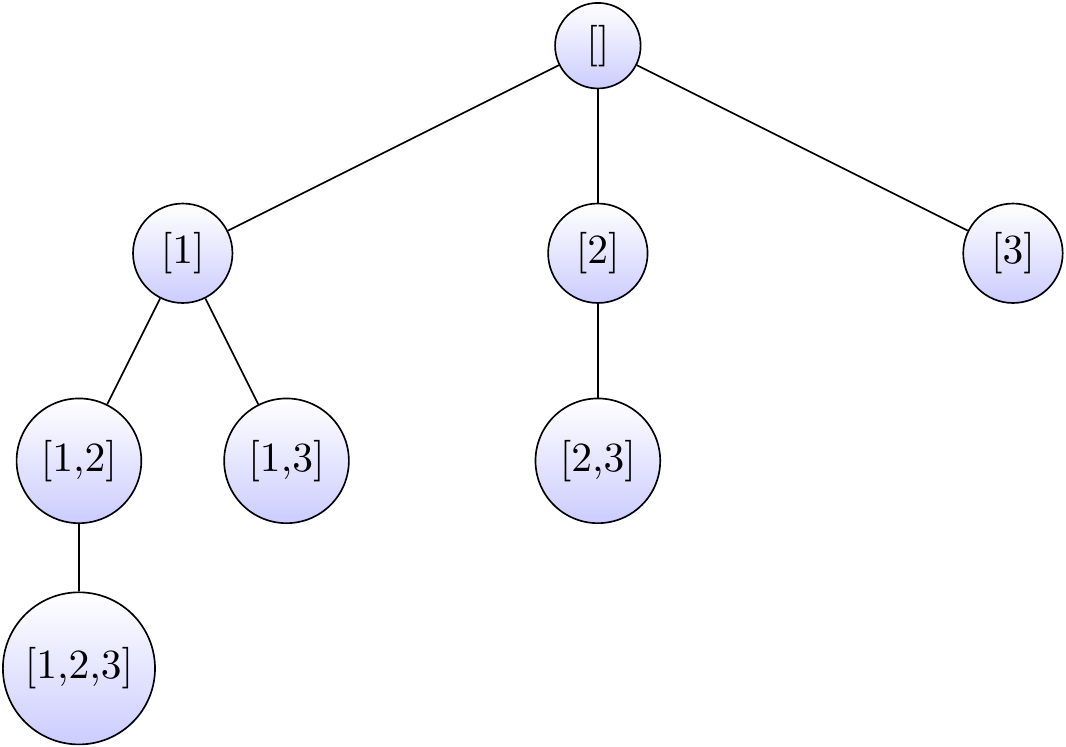
\includegraphics[width=0.9\linewidth]{bookdown-demo_files/figure-latex/unnamed-chunk-2-1} \caption{Some caption.}\label{fig:unnamed-chunk-2}
\end{figure}

Enumerate all possible result by adding a new element that is greater than current element while traversing the array.
Remember to backtrack.

\hypertarget{analysis-16}{%
\subsubsection{Analysis}\label{analysis-16}}

Time complexity between \(O(2^{n})\) as there are at most \(2^n\) subsets.

\hypertarget{algorithm-16}{%
\subsubsection{Algorithm}\label{algorithm-16}}

\{backtrack\}, \{recursive\}

\hypertarget{java-code-12}{%
\subsection{Java Code}\label{java-code-12}}

\begin{Shaded}
\begin{Highlighting}[]
\BuiltInTok{List}\NormalTok{<}\BuiltInTok{List}\NormalTok{<}\BuiltInTok{Integer}\NormalTok{>> result = }\KeywordTok{new} \BuiltInTok{ArrayList}\NormalTok{<>();}

\KeywordTok{public} \BuiltInTok{List}\NormalTok{<}\BuiltInTok{List}\NormalTok{<}\BuiltInTok{Integer}\NormalTok{>> }\FunctionTok{subsets}\NormalTok{(}\DataTypeTok{int}\NormalTok{[] nums) \{}
    \KeywordTok{if}\NormalTok{ (nums.}\FunctionTok{length}\NormalTok{ == }\DecValTok{0}\NormalTok{) \{}
        \KeywordTok{return}\NormalTok{ result;}
\NormalTok{    \}}

    \BuiltInTok{Arrays}\NormalTok{.}\FunctionTok{sort}\NormalTok{(nums);}

    \FunctionTok{backtrack}\NormalTok{(nums, }\DecValTok{0}\NormalTok{, }\KeywordTok{new} \BuiltInTok{ArrayList}\NormalTok{<>());}

    \KeywordTok{return}\NormalTok{ result;}
\NormalTok{\}}

\KeywordTok{private} \DataTypeTok{void} \FunctionTok{backtrack}\NormalTok{(}\DataTypeTok{int}\NormalTok{[] nums, }\DataTypeTok{int}\NormalTok{ index, }\BuiltInTok{List}\NormalTok{<}\BuiltInTok{Integer}\NormalTok{> list) \{}
    \CommentTok{//copy elements from the current list}
\NormalTok{    result.}\FunctionTok{add}\NormalTok{(}\KeywordTok{new} \BuiltInTok{ArrayList}\NormalTok{<>(list));}

    \KeywordTok{for}\NormalTok{(}\DataTypeTok{int}\NormalTok{ i = index; i < nums.}\FunctionTok{length}\NormalTok{; i++) \{}
\NormalTok{        list.}\FunctionTok{add}\NormalTok{(nums[i]);}
        \FunctionTok{backtrack}\NormalTok{(nums, i + }\DecValTok{1}\NormalTok{, list);}

        \CommentTok{//remove last element to backtrack}
\NormalTok{        list.}\FunctionTok{remove}\NormalTok{(list.}\FunctionTok{size}\NormalTok{() - }\DecValTok{1}\NormalTok{);}
\NormalTok{    \}}
\NormalTok{\}}
\end{Highlighting}
\end{Shaded}

\hypertarget{subsets-ii-leetcode-90-medium}{%
\section{Subsets II / LeetCode 90 / Medium\}}\label{subsets-ii-leetcode-90-medium}}

\hypertarget{description-16}{%
\subsection{Description}\label{description-16}}

Given a collection of integers that might contain duplicates, nums, return all possible subsets (the power set).

Note: The solution set must not contain duplicate subsets.

\hypertarget{example-15}{%
\subsection{Example}\label{example-15}}

Input: nums = {[}1,2,2{]}, Output:

\begin{Shaded}
\begin{Highlighting}[]
\NormalTok{[}
\NormalTok{    [}\DecValTok{2}\NormalTok{],}
\NormalTok{    [}\DecValTok{1}\NormalTok{],}
\NormalTok{    [}\DecValTok{1}\NormalTok{,}\DecValTok{2}\NormalTok{,}\DecValTok{2}\NormalTok{],}
\NormalTok{    [}\DecValTok{2}\NormalTok{,}\DecValTok{2}\NormalTok{],}
\NormalTok{    [}\DecValTok{1}\NormalTok{,}\DecValTok{2}\NormalTok{],}
\NormalTok{    []}
\NormalTok{]}
\end{Highlighting}
\end{Shaded}

\hypertarget{solution-11}{%
\subsection{Solution}\label{solution-11}}

\hypertarget{walkthrough-15}{%
\subsubsection{Walkthrough}\label{walkthrough-15}}

The enumeration tree is as the following:

\begin{figure}
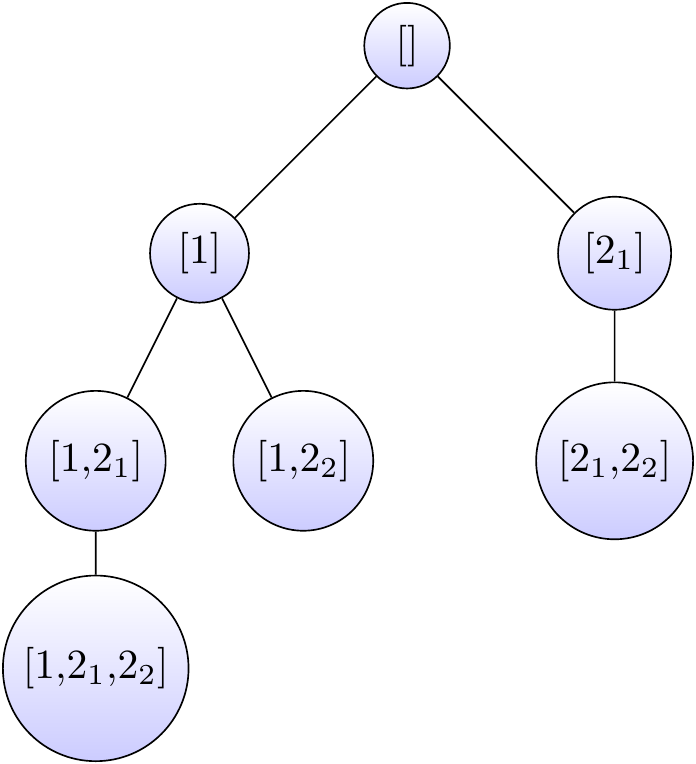
\includegraphics[width=0.9\linewidth]{bookdown-demo_files/figure-latex/unnamed-chunk-3-1} \caption{Some caption.}\label{fig:unnamed-chunk-3}
\end{figure}

Enumerate all possible result by adding a new element that is greater than current element while traversing the array.
Skip if two consecutive elements are the same. Remember to backtrack.

\hypertarget{analysis-17}{%
\subsubsection{Analysis}\label{analysis-17}}

Time complexity between \(O(2^{n})\) as there are at most \(2^n\) subsets.

\hypertarget{algorithm-17}{%
\subsubsection{Algorithm}\label{algorithm-17}}

\{backtrack\}, \{recursive\}

\hypertarget{java-code-13}{%
\subsection{Java Code}\label{java-code-13}}

\begin{Shaded}
\begin{Highlighting}[]
\BuiltInTok{List}\NormalTok{<}\BuiltInTok{List}\NormalTok{<}\BuiltInTok{Integer}\NormalTok{>> result = }\KeywordTok{new} \BuiltInTok{ArrayList}\NormalTok{<>();}

\KeywordTok{public} \BuiltInTok{List}\NormalTok{<}\BuiltInTok{List}\NormalTok{<}\BuiltInTok{Integer}\NormalTok{>> }\FunctionTok{subsetsWithDup}\NormalTok{(}\DataTypeTok{int}\NormalTok{[] nums) \{}
    \KeywordTok{if}\NormalTok{ (nums.}\FunctionTok{length}\NormalTok{ == }\DecValTok{0}\NormalTok{) \{}
        \KeywordTok{return}\NormalTok{ result;}
\NormalTok{    \}}

    \BuiltInTok{Arrays}\NormalTok{.}\FunctionTok{sort}\NormalTok{(nums);}
    \FunctionTok{backtrack}\NormalTok{(nums, }\DecValTok{0}\NormalTok{, }\KeywordTok{new} \BuiltInTok{ArrayList}\NormalTok{<>());}

    \KeywordTok{return}\NormalTok{ result;}
\NormalTok{\}}

\KeywordTok{private} \DataTypeTok{void} \FunctionTok{backtrack}\NormalTok{(}\DataTypeTok{int}\NormalTok{[] nums, }\DataTypeTok{int}\NormalTok{ index, }\BuiltInTok{List}\NormalTok{<}\BuiltInTok{Integer}\NormalTok{> list) \{}
    \CommentTok{//copy elements from the current list}
\NormalTok{    result.}\FunctionTok{add}\NormalTok{(}\KeywordTok{new} \BuiltInTok{ArrayList}\NormalTok{<>(list));}

    \KeywordTok{for}\NormalTok{(}\DataTypeTok{int}\NormalTok{ i = index; i < nums.}\FunctionTok{length}\NormalTok{; i++) \{}
        \KeywordTok{if}\NormalTok{(i != index && nums[i] == nums[i - }\DecValTok{1}\NormalTok{]) \{}
            \KeywordTok{continue}\NormalTok{;}
\NormalTok{        \}}

\NormalTok{        list.}\FunctionTok{add}\NormalTok{(nums[i]);}
        \FunctionTok{backtrack}\NormalTok{(nums, i + }\DecValTok{1}\NormalTok{, list);}

        \CommentTok{//remove last element to backtrack}
\NormalTok{        list.}\FunctionTok{remove}\NormalTok{(list.}\FunctionTok{size}\NormalTok{() - }\DecValTok{1}\NormalTok{);}
\NormalTok{    \}}
\NormalTok{\}}
\end{Highlighting}
\end{Shaded}

\hypertarget{sort-array-by-parity-leetcode-906-easy}{%
\section{Sort Array By Parity / LeetCode 906 / Easy\}}\label{sort-array-by-parity-leetcode-906-easy}}

\hypertarget{description-17}{%
\subsection{Description}\label{description-17}}

Given an array A of non-negative integers, return an array consisting of all the even elements of A, followed by all
the odd elements of A.

You may return any answer array that satisfies this condition.

\hypertarget{example-16}{%
\subsection{Example}\label{example-16}}

Input: {[}3,1,2,4{]}. Output: {[}2,4,3,1{]}. The outputs {[}4,2,3,1{]}, {[}2,4,1,3{]}, and {[}4,2,1,3{]} would also be accepted.

\hypertarget{solution-12}{%
\subsection{Solution}\label{solution-12}}

\hypertarget{walkthrough-16}{%
\subsubsection{Walkthrough}\label{walkthrough-16}}

Have two indices, left and right. Shrink both indices (left, right) where they satisfy the condition. Swap those
who do not and shrink both indices again.

\hypertarget{analysis-18}{%
\subsubsection{Analysis}\label{analysis-18}}

Complexity is \(O(n)\) since each element is visited once.

\hypertarget{algorithm-18}{%
\subsubsection{Algorithm}\label{algorithm-18}}

\hypertarget{java-code-14}{%
\subsection{Java Code}\label{java-code-14}}

\begin{Shaded}
\begin{Highlighting}[]
\KeywordTok{public} \DataTypeTok{int}\NormalTok{[] }\FunctionTok{sortArrayByParity}\NormalTok{(}\DataTypeTok{int}\NormalTok{[] A) \{}
    \KeywordTok{if}\NormalTok{(A == }\KeywordTok{null}\NormalTok{ || A.}\FunctionTok{length}\NormalTok{ == }\DecValTok{0}\NormalTok{) \{}
        \KeywordTok{return} \KeywordTok{null}\NormalTok{;}
\NormalTok{    \}}

    \DataTypeTok{int}\NormalTok{ l = }\DecValTok{0}\NormalTok{, r = A.}\FunctionTok{length}\NormalTok{ - }\DecValTok{1}\NormalTok{;}
    \KeywordTok{while}\NormalTok{(l < r) \{}
        \KeywordTok{while}\NormalTok{ (A[l]%}\DecValTok{2}\NormalTok{ == }\DecValTok{0}\NormalTok{ && l < r) \{}
            \CommentTok{//do nothing, incremnt left index}
\NormalTok{            l++;}
\NormalTok{        \}}

        \KeywordTok{while}\NormalTok{ (A[r]%}\DecValTok{2}\NormalTok{ == }\DecValTok{1}\NormalTok{ && l < r) \{}
            \CommentTok{//do nothing, decrement right index}
\NormalTok{            r--;}
\NormalTok{        \}}


        \KeywordTok{if}\NormalTok{( l < r ) \{}
            \CommentTok{//odd #, swap}
            \DataTypeTok{int}\NormalTok{ temp = A[l];}
\NormalTok{            A[l] = A[r];}
\NormalTok{            A[r] = temp;}

\NormalTok{            l++;}
\NormalTok{            r--;}
\NormalTok{        \}}
\NormalTok{    \}}

    \KeywordTok{return}\NormalTok{ A;}
\NormalTok{\}}
\end{Highlighting}
\end{Shaded}

\hypertarget{merge-intervals-leetcode-56-medium}{%
\section{Merge Intervals / LeetCode 56 / Medium\}}\label{merge-intervals-leetcode-56-medium}}

\hypertarget{description-18}{%
\subsection{Description}\label{description-18}}

Given a collection of intervals, merge all overlapping intervals.

\hypertarget{example-17}{%
\subsection{Example}\label{example-17}}

Input: {[}{[}1,3{]},{[}2,6{]},{[}8,10{]},{[}15,18{]}{]}. Output: {[}{[}1,6{]},{[}8,10{]},{[}15,18{]}{]}. Explanation: Since intervals {[}1,3{]} and {[}2,6{]} overlaps, merge them into {[}1,6{]}.

Input: {[}{[}1,4{]},{[}4,5{]}{]}. Output: {[}{[}1,5{]}{]}. Explanation: Intervals {[}1,4{]} and {[}4,5{]} are considered overlapping.

\hypertarget{solution-13}{%
\subsection{Solution}\label{solution-13}}

\hypertarget{walkthrough-17}{%
\subsubsection{Walkthrough}\label{walkthrough-17}}

Sort the list of intervals first. Use a stack to track the lastly pushed interval. If the current interval does
not overlap with the top interval, push current interval to stack. If there is an overlap, we merge the
current and previous interval.

\hypertarget{analysis-19}{%
\subsubsection{Analysis}\label{analysis-19}}

Complexity is : \(O(n \cdot log n)\) since we sort the array first.

\hypertarget{algorithm-19}{%
\subsubsection{Algorithm}\label{algorithm-19}}

\hypertarget{java-code-15}{%
\subsection{Java Code}\label{java-code-15}}

\begin{Shaded}
\begin{Highlighting}[]
\DataTypeTok{static} \KeywordTok{class}\NormalTok{ Interval \{}
    \DataTypeTok{int}\NormalTok{ start;}
    \DataTypeTok{int}\NormalTok{ end;}

    \KeywordTok{public} \FunctionTok{Interval}\NormalTok{(}\DataTypeTok{int}\NormalTok{ l, }\DataTypeTok{int}\NormalTok{ r) \{}
\NormalTok{        start = l;}
\NormalTok{        end = r;}
\NormalTok{    \}}
\NormalTok{\}}

\KeywordTok{public} \DataTypeTok{int}\NormalTok{[][] }\FunctionTok{merge}\NormalTok{(}\DataTypeTok{int}\NormalTok{[][] intervals) \{}
    \BuiltInTok{List}\NormalTok{<Interval> input = }\KeywordTok{new} \BuiltInTok{ArrayList}\NormalTok{<>();}
    \KeywordTok{for}\NormalTok{(}\DataTypeTok{int}\NormalTok{[] interval : intervals) \{}
\NormalTok{        input.}\FunctionTok{add}\NormalTok{(}\KeywordTok{new} \FunctionTok{Interval}\NormalTok{(interval[}\DecValTok{0}\NormalTok{], interval[}\DecValTok{1}\NormalTok{]));}
\NormalTok{    \}}

    \KeywordTok{if}\NormalTok{(intervals.}\FunctionTok{length}\NormalTok{ == }\DecValTok{0}\NormalTok{) \{}
        \KeywordTok{return} \KeywordTok{new} \DataTypeTok{int}\NormalTok{[}\DecValTok{0}\NormalTok{][}\DecValTok{0}\NormalTok{];}
\NormalTok{    \}}

    \BuiltInTok{List}\NormalTok{<Interval> output = }\FunctionTok{merge}\NormalTok{(input);}
    \DataTypeTok{int}\NormalTok{[][] result = }\KeywordTok{new} \DataTypeTok{int}\NormalTok{[output.}\FunctionTok{size}\NormalTok{()][}\DecValTok{2}\NormalTok{];}

    \KeywordTok{for}\NormalTok{(}\DataTypeTok{int}\NormalTok{ i = }\DecValTok{0}\NormalTok{; i < output.}\FunctionTok{size}\NormalTok{(); i++) \{}
\NormalTok{        result[i][}\DecValTok{0}\NormalTok{] = output.}\FunctionTok{get}\NormalTok{(i).}\FunctionTok{start}\NormalTok{;}
\NormalTok{        result[i][}\DecValTok{1}\NormalTok{] = output.}\FunctionTok{get}\NormalTok{(i).}\FunctionTok{end}\NormalTok{;}
\NormalTok{    \}}

    \KeywordTok{return}\NormalTok{ result;}
\NormalTok{\}}

\KeywordTok{private} \KeywordTok{class}\NormalTok{ IntervalComparator }\KeywordTok{implements} \BuiltInTok{Comparator}\NormalTok{<Interval> \{}
    \AttributeTok{@Override}
    \KeywordTok{public} \DataTypeTok{int} \FunctionTok{compare}\NormalTok{(Interval a, Interval b) \{}
        \KeywordTok{return}\NormalTok{ a.}\FunctionTok{start}\NormalTok{ - b.}\FunctionTok{start}\NormalTok{;}
\NormalTok{    \}}
\NormalTok{\}}

\KeywordTok{public} \BuiltInTok{List}\NormalTok{<Interval> }\FunctionTok{merge}\NormalTok{(}\BuiltInTok{List}\NormalTok{<Interval> intervals) \{}
    \CommentTok{//sort the list}
    \BuiltInTok{Collections}\NormalTok{.}\FunctionTok{sort}\NormalTok{(intervals, }\KeywordTok{new} \FunctionTok{IntervalComparator}\NormalTok{());}

    \BuiltInTok{Stack}\NormalTok{<Interval> merged = }\KeywordTok{new} \BuiltInTok{Stack}\NormalTok{<Interval>();}
\NormalTok{    merged.}\FunctionTok{push}\NormalTok{(intervals.}\FunctionTok{get}\NormalTok{(}\DecValTok{0}\NormalTok{));}

    \KeywordTok{for}\NormalTok{ (}\DataTypeTok{int}\NormalTok{ i = }\DecValTok{1}\NormalTok{; i < intervals.}\FunctionTok{size}\NormalTok{(); i++) \{}
\NormalTok{        Interval interval = intervals.}\FunctionTok{get}\NormalTok{(i);}
\NormalTok{        Interval top = merged.}\FunctionTok{peek}\NormalTok{();}

        \CommentTok{// if interval does not overlap with the previous, simply append it.}
        \KeywordTok{if}\NormalTok{ (top.}\FunctionTok{end}\NormalTok{ < interval.}\FunctionTok{start}\NormalTok{) \{}
\NormalTok{            merged.}\FunctionTok{push}\NormalTok{(interval);}
\NormalTok{        \}}
        \CommentTok{// if there is an overlap, we merge the current with the last interval}
        \CommentTok{// by comparing their end boundaries}
        \KeywordTok{else}\NormalTok{ \{}
\NormalTok{            top.}\FunctionTok{end}\NormalTok{ = }\BuiltInTok{Math}\NormalTok{.}\FunctionTok{max}\NormalTok{(top.}\FunctionTok{end}\NormalTok{, interval.}\FunctionTok{end}\NormalTok{);}
\NormalTok{        \}}
\NormalTok{    \}}

    \KeywordTok{return}\NormalTok{ merged;}
\NormalTok{\}}
\end{Highlighting}
\end{Shaded}

\hypertarget{non-overlapping-intervals-leetcode-435-medium}{%
\section{Non-overlapping Intervals / LeetCode 435 / Medium\}}\label{non-overlapping-intervals-leetcode-435-medium}}

\hypertarget{description-19}{%
\subsection{Description}\label{description-19}}

Given a collection of intervals, find the minimum number of intervals you need to remove to make the rest of the
intervals non-overlapping.

\hypertarget{example-18}{%
\subsection{Example}\label{example-18}}

Input: {[}{[}1,2{]},{[}2,3{]},{[}3,4{]},{[}1,3{]}{]}. Output: 1 Explanation: {[}1,3{]} can be removed and the rest of intervals are
non-overlapping.

Input: {[}{[}1,2{]},{[}1,2{]},{[}1,2{]}{]}. Output: 2 . Explanation: You need to remove two {[}1,2{]} to make the rest of intervals
non-overlapping.

\hypertarget{solution-14}{%
\subsection{Solution}\label{solution-14}}

\hypertarget{walkthrough-18}{%
\subsubsection{Walkthrough}\label{walkthrough-18}}

First, sort the array and count non-overlapping interval - not overlapped with previous end. Finally, number of
overlapping intervals would be n - count.

\hypertarget{analysis-20}{%
\subsubsection{Analysis}\label{analysis-20}}

Complexity is \(O(n \cdot log n)\) because of sorting ahead.

\hypertarget{algorithm-20}{%
\subsubsection{Algorithm}\label{algorithm-20}}

\hypertarget{java-code-16}{%
\subsection{Java Code}\label{java-code-16}}

\begin{Shaded}
\begin{Highlighting}[]
\KeywordTok{public} \DataTypeTok{int} \FunctionTok{eraseOverlapIntervals}\NormalTok{(}\DataTypeTok{int}\NormalTok{[][] intervals) \{}
    \KeywordTok{if}\NormalTok{(intervals == }\KeywordTok{null}\NormalTok{ || intervals.}\FunctionTok{length}\NormalTok{ == }\DecValTok{0}\NormalTok{) \{}
        \KeywordTok{return} \DecValTok{0}\NormalTok{;}
\NormalTok{    \}}

    \BuiltInTok{Arrays}\NormalTok{.}\FunctionTok{sort}\NormalTok{(intervals, }\KeywordTok{new} \BuiltInTok{Comparator}\NormalTok{<}\DataTypeTok{int}\NormalTok{[]>() \{}
        \AttributeTok{@Override}
        \KeywordTok{public} \DataTypeTok{int} \FunctionTok{compare}\NormalTok{(}\DataTypeTok{int}\NormalTok{[] i1, }\DataTypeTok{int}\NormalTok{[] i2) \{}
            \KeywordTok{if}\NormalTok{ (i1[}\DecValTok{1}\NormalTok{] != i2[}\DecValTok{1}\NormalTok{])\{}
                \CommentTok{//compare end time}
                \KeywordTok{return}\NormalTok{ i1[}\DecValTok{1}\NormalTok{] - i2[}\DecValTok{1}\NormalTok{];}
\NormalTok{            \}}\KeywordTok{else}\NormalTok{ \{}
                \CommentTok{//compare start time}
                \KeywordTok{return}\NormalTok{ i1[}\DecValTok{0}\NormalTok{] - i2[}\DecValTok{0}\NormalTok{];}
\NormalTok{            \}}
\NormalTok{        \}}
\NormalTok{    \});}

    \CommentTok{//end for latest non-overlapped interval}
    \DataTypeTok{int}\NormalTok{ end = intervals[}\DecValTok{0}\NormalTok{][}\DecValTok{1}\NormalTok{];}
    \DataTypeTok{int}\NormalTok{ n = intervals.}\FunctionTok{length}\NormalTok{;}
    \DataTypeTok{int}\NormalTok{ count = }\DecValTok{1}\NormalTok{;}

    \KeywordTok{for}\NormalTok{ (}\DataTypeTok{int}\NormalTok{ i = }\DecValTok{1}\NormalTok{; i < n; i++) \{}
        \KeywordTok{if}\NormalTok{ (intervals[i][}\DecValTok{0}\NormalTok{] >= end) \{}
            \CommentTok{//for any non-overlapped interval, update end & count}
\NormalTok{            end = intervals[i][}\DecValTok{1}\NormalTok{];}
\NormalTok{            count++;}
\NormalTok{        \}}
\NormalTok{    \}}

    \KeywordTok{return}\NormalTok{ n - count;}
\NormalTok{\}}
\end{Highlighting}
\end{Shaded}

\hypertarget{interval-list-intersections-leetcode-986-medium}{%
\section{Interval List Intersections / LeetCode 986 / Medium\}}\label{interval-list-intersections-leetcode-986-medium}}

\hypertarget{description-20}{%
\subsection{Description}\label{description-20}}

Given two lists of closed intervals, each list of intervals is pairwise disjoint and in sorted order.
Return the intersection of these two interval lists.

\hypertarget{example-19}{%
\subsection{Example}\label{example-19}}

Input: A = {[}{[}0,2{]},{[}5,10{]},{[}13,23{]},{[}24,25{]}{]}, B = {[}{[}1,5{]},{[}8,12{]},{[}15,24{]},{[}25,26{]}{]}
Output: {[}{[}1,2{]},{[}5,5{]},{[}8,10{]},{[}15,23{]},{[}24,24{]},{[}25,25{]}{]}
Reminder: The inputs and the desired output are lists of Interval objects, and not arrays or lists.

\hypertarget{solution-15}{%
\subsection{Solution}\label{solution-15}}

\hypertarget{walkthrough-19}{%
\subsubsection{Walkthrough}\label{walkthrough-19}}

Traverse the two lists of intervals. Merge two intervals if there is an intersection. Move the index of A if
\(A[i]\).end \(< B[i]\).end since the interval is the smaller out of comparison.

\hypertarget{analysis-21}{%
\subsubsection{Analysis}\label{analysis-21}}

The runtime complexity is \(O(n * m)\)

\hypertarget{algorithm-21}{%
\subsubsection{Algorithm}\label{algorithm-21}}

\hypertarget{java-code-17}{%
\subsection{Java Code}\label{java-code-17}}

\begin{Shaded}
\begin{Highlighting}[]
\NormalTok{LeetCode }\DecValTok{986}\NormalTok{ / Medium}
\KeywordTok{private} \DataTypeTok{static} \KeywordTok{class}\NormalTok{ Interval \{}
    \KeywordTok{public} \DataTypeTok{int}\NormalTok{ start;}
    \KeywordTok{public} \DataTypeTok{int}\NormalTok{ end;}

    \KeywordTok{public} \FunctionTok{Interval}\NormalTok{(}\DataTypeTok{int}\NormalTok{ s, }\DataTypeTok{int}\NormalTok{ e) \{}
        \KeywordTok{this}\NormalTok{.}\FunctionTok{start}\NormalTok{ = s;}
        \KeywordTok{this}\NormalTok{.}\FunctionTok{end}\NormalTok{ = e;}
\NormalTok{    \}}

    \KeywordTok{public} \DataTypeTok{static} \DataTypeTok{int}\NormalTok{[][] }\FunctionTok{toArray}\NormalTok{(}\BuiltInTok{List}\NormalTok{<Interval> list) \{}
        \DataTypeTok{int}\NormalTok{[][] result = }\KeywordTok{new} \DataTypeTok{int}\NormalTok{[list.}\FunctionTok{size}\NormalTok{()][}\DecValTok{2}\NormalTok{];}

        \KeywordTok{for}\NormalTok{(}\DataTypeTok{int}\NormalTok{ i = }\DecValTok{0}\NormalTok{; i < list.}\FunctionTok{size}\NormalTok{(); i++) \{}
\NormalTok{            Interval interval = list.}\FunctionTok{get}\NormalTok{(i);}

\NormalTok{            result[i] = }\KeywordTok{new} \DataTypeTok{int}\NormalTok{[] \{interval.}\FunctionTok{start}\NormalTok{, interval.}\FunctionTok{end}\NormalTok{\};}
\NormalTok{        \}}

        \KeywordTok{return}\NormalTok{ result;}
\NormalTok{    \}}

    \KeywordTok{public} \DataTypeTok{static} \BuiltInTok{List}\NormalTok{<Interval> }\FunctionTok{toList}\NormalTok{(}\DataTypeTok{int}\NormalTok{[][] array) \{}
        \BuiltInTok{List}\NormalTok{<Interval> result = }\KeywordTok{new} \BuiltInTok{ArrayList}\NormalTok{<>();}

        \KeywordTok{for}\NormalTok{(}\DataTypeTok{int}\NormalTok{ i = }\DecValTok{0}\NormalTok{; i < array.}\FunctionTok{length}\NormalTok{; i++) \{}
\NormalTok{            Interval interval = }\KeywordTok{new} \FunctionTok{Interval}\NormalTok{(array[i][}\DecValTok{0}\NormalTok{], array[i][}\DecValTok{1}\NormalTok{]);}

\NormalTok{            result.}\FunctionTok{add}\NormalTok{(interval);}
\NormalTok{        \}}

        \KeywordTok{return}\NormalTok{ result;}
\NormalTok{    \}}

\NormalTok{\}}
\KeywordTok{public} \DataTypeTok{int}\NormalTok{[][] }\FunctionTok{intervalIntersection}\NormalTok{(}\DataTypeTok{int}\NormalTok{[][] A, }\DataTypeTok{int}\NormalTok{[][] B) \{}
    \BuiltInTok{List}\NormalTok{<Interval> intervalsA = Interval.}\FunctionTok{toList}\NormalTok{(A);}
    \BuiltInTok{List}\NormalTok{<Interval> intervalsB = Interval.}\FunctionTok{toList}\NormalTok{(B);}
    \BuiltInTok{List}\NormalTok{<Interval> result = }\KeywordTok{new} \BuiltInTok{ArrayList}\NormalTok{<>();}

    \DataTypeTok{int}\NormalTok{ i = }\DecValTok{0}\NormalTok{, j = }\DecValTok{0}\NormalTok{;}
    \KeywordTok{while}\NormalTok{( i < intervalsA.}\FunctionTok{size}\NormalTok{() && j < intervalsB.}\FunctionTok{size}\NormalTok{()) \{}
        \DataTypeTok{int}\NormalTok{ highStart = }\BuiltInTok{Math}\NormalTok{.}\FunctionTok{max}\NormalTok{(intervalsA.}\FunctionTok{get}\NormalTok{(i).}\FunctionTok{start}\NormalTok{, intervalsB.}\FunctionTok{get}\NormalTok{(j).}\FunctionTok{start}\NormalTok{);}
        \DataTypeTok{int}\NormalTok{ lowEnd = }\BuiltInTok{Math}\NormalTok{.}\FunctionTok{min}\NormalTok{(intervalsA.}\FunctionTok{get}\NormalTok{(i).}\FunctionTok{end}\NormalTok{, intervalsB.}\FunctionTok{get}\NormalTok{(j).}\FunctionTok{end}\NormalTok{);}

        \CommentTok{//there is an intersection}
        \KeywordTok{if}\NormalTok{( highStart <= lowEnd) \{}
\NormalTok{            result.}\FunctionTok{add}\NormalTok{( }\KeywordTok{new} \FunctionTok{Interval}\NormalTok{(highStart, lowEnd));}
\NormalTok{        \}}
        \KeywordTok{if}\NormalTok{( intervalsA.}\FunctionTok{get}\NormalTok{(i).}\FunctionTok{end}\NormalTok{ < intervalsB.}\FunctionTok{get}\NormalTok{(j).}\FunctionTok{end}\NormalTok{) \{}
            \CommentTok{//move index of A[]}
\NormalTok{            i++;}
\NormalTok{        \} }\KeywordTok{else}\NormalTok{ \{}
            \CommentTok{//move index of B[]}
\NormalTok{            j++;}
\NormalTok{        \}}
\NormalTok{    \}}

    \KeywordTok{return}\NormalTok{ Interval.}\FunctionTok{toArray}\NormalTok{(result);}
\NormalTok{\}}
\end{Highlighting}
\end{Shaded}

\hypertarget{insert-interval-leetcode-57-hard}{%
\section{Insert Interval / LeetCode 57 / Hard\}}\label{insert-interval-leetcode-57-hard}}

\hypertarget{description-21}{%
\subsection{Description}\label{description-21}}

Given a set of non-overlapping intervals, insert a new interval into the intervals (merge if necessary).

You may assume that the intervals were initially sorted according to their start times.

\hypertarget{example-20}{%
\subsection{Example}\label{example-20}}

Input: intervals = {[}{[}1,3{]},{[}6,9{]}{]}, newInterval = {[}2,5{]} Output: {[}{[}1,5{]},{[}6,9{]}{]}

Input: intervals = {[}{[}1,2{]},{[}3,5{]},{[}6,7{]},{[}8,10{]},{[}12,16{]}{]}, newInterval = {[}4,8{]}. Output: {[}{[}1,2{]},{[}3,10{]},{[}12,16{]}{]}
Explanation: Because the new interval {[}4,8{]} overlaps with {[}3,5{]},{[}6,7{]},{[}8,10{]}.

\hypertarget{solution-16}{%
\subsection{Solution}\label{solution-16}}

\hypertarget{walkthrough-20}{%
\subsubsection{Walkthrough}\label{walkthrough-20}}

Leverage the merge() method to find out which intervals can be merged with new Inserted interval.

\hypertarget{analysis-22}{%
\subsubsection{Analysis}\label{analysis-22}}

Time complexity is \(O(n \cdot log(n))\) because of sorting ahead.

\hypertarget{algorithm-22}{%
\subsubsection{Algorithm}\label{algorithm-22}}

\hypertarget{java-code-18}{%
\subsection{Java Code}\label{java-code-18}}

\begin{Shaded}
\begin{Highlighting}[]
\KeywordTok{private} \DataTypeTok{static} \KeywordTok{class}\NormalTok{ Interval \{}
    \KeywordTok{public} \DataTypeTok{int}\NormalTok{ start;}
    \KeywordTok{public} \DataTypeTok{int}\NormalTok{ end;}

    \KeywordTok{public} \FunctionTok{Interval}\NormalTok{(}\DataTypeTok{int}\NormalTok{ s, }\DataTypeTok{int}\NormalTok{ e) \{}
        \KeywordTok{this}\NormalTok{.}\FunctionTok{start}\NormalTok{ = s;}
        \KeywordTok{this}\NormalTok{.}\FunctionTok{end}\NormalTok{ = e;}
\NormalTok{    \}}

    \KeywordTok{public} \DataTypeTok{static} \DataTypeTok{int}\NormalTok{[][] }\FunctionTok{toArray}\NormalTok{(}\BuiltInTok{List}\NormalTok{<Interval> list) \{}
        \DataTypeTok{int}\NormalTok{[][] result = }\KeywordTok{new} \DataTypeTok{int}\NormalTok{[list.}\FunctionTok{size}\NormalTok{()][}\DecValTok{2}\NormalTok{];}

        \KeywordTok{for}\NormalTok{(}\DataTypeTok{int}\NormalTok{ i = }\DecValTok{0}\NormalTok{; i < list.}\FunctionTok{size}\NormalTok{(); i++) \{}
\NormalTok{            Interval interval = list.}\FunctionTok{get}\NormalTok{(i);}

\NormalTok{            result[i] = }\KeywordTok{new} \DataTypeTok{int}\NormalTok{[] \{interval.}\FunctionTok{start}\NormalTok{, interval.}\FunctionTok{end}\NormalTok{\};}
\NormalTok{        \}}

        \KeywordTok{return}\NormalTok{ result;}
\NormalTok{    \}}

    \KeywordTok{public} \DataTypeTok{static} \BuiltInTok{List}\NormalTok{<Interval> }\FunctionTok{toList}\NormalTok{(}\DataTypeTok{int}\NormalTok{[][] array) \{}
        \BuiltInTok{List}\NormalTok{<Interval> result = }\KeywordTok{new} \BuiltInTok{ArrayList}\NormalTok{<>();}

        \KeywordTok{for}\NormalTok{(}\DataTypeTok{int}\NormalTok{ i = }\DecValTok{0}\NormalTok{; i < array.}\FunctionTok{length}\NormalTok{; i++) \{}
\NormalTok{            Interval interval = }\KeywordTok{new} \FunctionTok{Interval}\NormalTok{(array[i][}\DecValTok{0}\NormalTok{], array[i][}\DecValTok{1}\NormalTok{]);}

\NormalTok{            result.}\FunctionTok{add}\NormalTok{(interval);}
\NormalTok{        \}}

        \KeywordTok{return}\NormalTok{ result;}
\NormalTok{    \}}
\NormalTok{\}}

\KeywordTok{public} \DataTypeTok{int}\NormalTok{[][] }\FunctionTok{insert}\NormalTok{(}\DataTypeTok{int}\NormalTok{[][] existed, }\DataTypeTok{int}\NormalTok{[] target) \{}
    \BuiltInTok{List}\NormalTok{<Interval> intervals = Interval.}\FunctionTok{toList}\NormalTok{(existed);}
\NormalTok{    Interval newInterval = }\KeywordTok{new} \FunctionTok{Interval}\NormalTok{(target[}\DecValTok{0}\NormalTok{], target[}\DecValTok{1}\NormalTok{]);}

\NormalTok{    intervals.}\FunctionTok{add}\NormalTok{(newInterval);}

    \BuiltInTok{List}\NormalTok{<Interval> merged = }\FunctionTok{merge}\NormalTok{(intervals);}

    \KeywordTok{return}\NormalTok{ Interval.}\FunctionTok{toArray}\NormalTok{(merged);}
\NormalTok{\}}

\KeywordTok{private} \KeywordTok{class}\NormalTok{ IntervalComparator }\KeywordTok{implements} \BuiltInTok{Comparator}\NormalTok{<Interval> \{}
    \AttributeTok{@Override}
    \KeywordTok{public} \DataTypeTok{int} \FunctionTok{compare}\NormalTok{(Interval a, Interval b) \{}
        \KeywordTok{return}\NormalTok{ a.}\FunctionTok{start}\NormalTok{ < b.}\FunctionTok{start}\NormalTok{ ? }\DecValTok{-1}\NormalTok{ : a.}\FunctionTok{start}\NormalTok{ == b.}\FunctionTok{start}\NormalTok{ ? }\DecValTok{0}\NormalTok{ : }\DecValTok{1}\NormalTok{;}
\NormalTok{    \}}
\NormalTok{\}}

\KeywordTok{public} \BuiltInTok{List}\NormalTok{<Interval> }\FunctionTok{merge}\NormalTok{(}\BuiltInTok{List}\NormalTok{<Interval> intervals) \{}
    \CommentTok{//sort the list}
    \BuiltInTok{Collections}\NormalTok{.}\FunctionTok{sort}\NormalTok{(intervals, }\KeywordTok{new} \FunctionTok{IntervalComparator}\NormalTok{());}

    \BuiltInTok{LinkedList}\NormalTok{<Interval> merged = }\KeywordTok{new} \BuiltInTok{LinkedList}\NormalTok{<Interval>();}
    \KeywordTok{for}\NormalTok{ (Interval interval : intervals) \{}
        \KeywordTok{if}\NormalTok{ (merged.}\FunctionTok{isEmpty}\NormalTok{() || merged.}\FunctionTok{getLast}\NormalTok{().}\FunctionTok{end}\NormalTok{ < interval.}\FunctionTok{start}\NormalTok{) \{}
            \CommentTok{// if the list of merged intervals is empty or if the current}
            \CommentTok{// interval does not overlap with the previous, simply append it.}
\NormalTok{            merged.}\FunctionTok{add}\NormalTok{(interval);}
\NormalTok{        \} }\KeywordTok{else}\NormalTok{ \{}
            \CommentTok{// otherwise, there is overlap, so we merge the current and previous}
            \CommentTok{// intervals.}
\NormalTok{            merged.}\FunctionTok{getLast}\NormalTok{().}\FunctionTok{end}\NormalTok{ = }\BuiltInTok{Math}\NormalTok{.}\FunctionTok{max}\NormalTok{(merged.}\FunctionTok{getLast}\NormalTok{().}\FunctionTok{end}\NormalTok{, interval.}\FunctionTok{end}\NormalTok{);}
\NormalTok{        \}}
\NormalTok{    \}}
    \KeywordTok{return}\NormalTok{ merged;}
\NormalTok{\}}
\end{Highlighting}
\end{Shaded}

\hypertarget{find-common-characters-leetcode-1002-easy}{%
\section{Find Common Characters / LeetCode 1002 / Easy\}}\label{find-common-characters-leetcode-1002-easy}}

\hypertarget{description-22}{%
\subsection{Description}\label{description-22}}

Given an array A of strings made only from lowercase letters, return a list of all characters that show up in all
strings within the list (including duplicates). For example, if a character occurs 3 times in all strings but
not 4 times, you need to include that character three times in the final answer. You may return the answer in
any order.

\hypertarget{example-21}{%
\subsection{Example}\label{example-21}}

Input: {[}``bella'',``label'',``roller''{]}. Output: {[}``e'',``l'',``l''{]}

Input: {[}``cool'',``lock'',``cook''{]}. Output: {[}``c'',``o''{]}

\hypertarget{solution-17}{%
\subsection{Solution}\label{solution-17}}

\hypertarget{walkthrough-21}{%
\subsubsection{Walkthrough}\label{walkthrough-21}}

First retrieve the alphabet distribution for the first word. For each of following word, maintain the min number
of duplicated alphabets. Lastly, take the alphabet which has more than 1 occurrences.

\hypertarget{analysis-23}{%
\subsubsection{Analysis}\label{analysis-23}}

Time complexity is O(n) where n is the number of words.

\hypertarget{algorithm-23}{%
\subsubsection{Algorithm}\label{algorithm-23}}

\hypertarget{java-code-19}{%
\subsection{Java Code}\label{java-code-19}}

\begin{Shaded}
\begin{Highlighting}[]
\KeywordTok{public} \BuiltInTok{List}\NormalTok{<}\BuiltInTok{String}\NormalTok{> }\FunctionTok{commonChars}\NormalTok{(}\BuiltInTok{String}\NormalTok{[] A) \{}
    \DataTypeTok{int}\NormalTok{[] minFreq = }\KeywordTok{new} \DataTypeTok{int}\NormalTok{[}\DecValTok{26}\NormalTok{];}

    \CommentTok{//init frequency map with the first string}
    \KeywordTok{for}\NormalTok{(}\DataTypeTok{int}\NormalTok{ i = }\DecValTok{0}\NormalTok{; i < A[}\DecValTok{0}\NormalTok{].}\FunctionTok{length}\NormalTok{(); i++) \{}
        \DataTypeTok{char}\NormalTok{ c = A[}\DecValTok{0}\NormalTok{].}\FunctionTok{charAt}\NormalTok{(i);}

        \DataTypeTok{int}\NormalTok{ index = c - }\CharTok{'a'}\NormalTok{;}
        \DataTypeTok{int}\NormalTok{ counter = minFreq[index];}
\NormalTok{        minFreq[index] = ++counter;}
\NormalTok{    \}}


    \CommentTok{//Do the actions for the following words}
    \KeywordTok{for}\NormalTok{(}\DataTypeTok{int}\NormalTok{ i = }\DecValTok{1}\NormalTok{; i < A.}\FunctionTok{length}\NormalTok{; i++) \{}
        \BuiltInTok{String}\NormalTok{ str = A[i];}
        \DataTypeTok{int}\NormalTok{[] tempFreq = }\KeywordTok{new} \DataTypeTok{int}\NormalTok{[}\DecValTok{26}\NormalTok{];}

        \CommentTok{//1. Store the frequency of alphabets}
        \KeywordTok{for}\NormalTok{(}\DataTypeTok{int}\NormalTok{ j = }\DecValTok{0}\NormalTok{; j < str.}\FunctionTok{length}\NormalTok{(); j++) \{}
            \DataTypeTok{char}\NormalTok{ c = str.}\FunctionTok{charAt}\NormalTok{(j);}

            \DataTypeTok{int}\NormalTok{ index = c - }\CharTok{'a'}\NormalTok{;}
            \DataTypeTok{int}\NormalTok{ counter = tempFreq[index];}
\NormalTok{            tempFreq[index] = ++counter;}
\NormalTok{        \}}

        \CommentTok{//2. Iterate thru 2 arrays and get the min number of (duplicated) alphabets}
        \CommentTok{//   non-duplicated returns 0}
        \KeywordTok{for}\NormalTok{(}\DataTypeTok{int}\NormalTok{ j = }\DecValTok{0}\NormalTok{; j < }\DecValTok{26}\NormalTok{; j++) \{}
\NormalTok{            minFreq[j] = }\BuiltInTok{Math}\NormalTok{.}\FunctionTok{min}\NormalTok{(minFreq[j], tempFreq[j]);}
\NormalTok{        \}}
\NormalTok{    \}}

    \DataTypeTok{int}\NormalTok{ numOfWords = A.}\FunctionTok{length}\NormalTok{;}
    \BuiltInTok{List}\NormalTok{<}\BuiltInTok{String}\NormalTok{> result = }\KeywordTok{new} \BuiltInTok{ArrayList}\NormalTok{<>();}


    \KeywordTok{for}\NormalTok{(}\DataTypeTok{int}\NormalTok{ i = }\DecValTok{0}\NormalTok{; i < }\DecValTok{26}\NormalTok{; i++) \{}
        \DataTypeTok{int}\NormalTok{ minCounter = minFreq[i];}

        \CommentTok{//Take the min number of duplicated alphabets (1 min)}
        \KeywordTok{for}\NormalTok{(}\DataTypeTok{int}\NormalTok{ j = }\DecValTok{0}\NormalTok{; j < minCounter; j++) \{}
            \DataTypeTok{char}\NormalTok{ alphabet = (}\DataTypeTok{char}\NormalTok{) (}\CharTok{'a'}\NormalTok{ + i);}
\NormalTok{            result.}\FunctionTok{add}\NormalTok{(}\BuiltInTok{String}\NormalTok{.}\FunctionTok{valueOf}\NormalTok{(alphabet));}
\NormalTok{        \}}
\NormalTok{    \}}

    \KeywordTok{return}\NormalTok{ result;}
\NormalTok{\}}
\end{Highlighting}
\end{Shaded}

\hypertarget{top-k-frequently-appeared-elements-leet-code-347-medium}{%
\section{Top K Frequently Appeared Elements / Leet Code 347 / Medium\}}\label{top-k-frequently-appeared-elements-leet-code-347-medium}}

\hypertarget{description-23}{%
\subsection{Description}\label{description-23}}

Given a non-empty array of integers, return the k most frequent elements. You may assume k is always valid,
\$1 \le k \le \$ number of unique elements. Your algorithm's time complexity must be better than O(\(n log n\)), where n
is the array's size.

\hypertarget{example-22}{%
\subsection{Example}\label{example-22}}

Input: nums = {[}1,1,1,2,2,3{]}, k = 2 Output: {[}1,2{]}
\#\#\# Solution
\#\#\#\# Walkthrough

\begin{enumerate}
    \item We first gather the frequency of integer by count with a HashMap
    \item We sort the frequency map by comparing by value() in descending order and sort them in
    $List<Entry<Number, Frequency>>$.
    \item We could traverse the top K entries from the list in a loop.
\end{enumerate}

\hypertarget{analysis-24}{%
\subsubsection{Analysis}\label{analysis-24}}

Since we sort the frequency map, thus the time complexity is \(O(n \cdot log n)\), and Auxiliary Space is \(O(n)\) to
store several maps and list.

\hypertarget{algorithm-24}{%
\subsubsection{Algorithm}\label{algorithm-24}}

\hypertarget{java-code-20}{%
\subsection{Java Code}\label{java-code-20}}

\begin{Shaded}
\begin{Highlighting}[]
\KeywordTok{public} \BuiltInTok{List}\NormalTok{<}\BuiltInTok{Integer}\NormalTok{> }\FunctionTok{topKFrequent}\NormalTok{(}\DataTypeTok{int}\NormalTok{[] nums, }\DataTypeTok{int}\NormalTok{ k) \{}
    \BuiltInTok{Map}\NormalTok{<}\BuiltInTok{Integer}\NormalTok{, }\BuiltInTok{Integer}\NormalTok{> freq = }\KeywordTok{new} \BuiltInTok{HashMap}\NormalTok{<>();}

    \KeywordTok{for}\NormalTok{ (}\DataTypeTok{int}\NormalTok{ num : nums) \{}
        \DataTypeTok{int}\NormalTok{ count = freq.}\FunctionTok{getOrDefault}\NormalTok{(num, }\DecValTok{0}\NormalTok{);}
\NormalTok{        freq.}\FunctionTok{put}\NormalTok{(num, ++count);}
\NormalTok{    \}}

    \CommentTok{//Sort Map.Entry by comparing by value() in descending order}
    \BuiltInTok{List}\NormalTok{<}\BuiltInTok{Map}\NormalTok{.}\FunctionTok{Entry}\NormalTok{<}\BuiltInTok{Integer}\NormalTok{, }\BuiltInTok{Integer}\NormalTok{>> sortedList = }\KeywordTok{new} \BuiltInTok{ArrayList}\NormalTok{<>(freq.}\FunctionTok{entrySet}\NormalTok{());}
\NormalTok{    sortedList.}\FunctionTok{sort}\NormalTok{(}\BuiltInTok{Map}\NormalTok{.}\FunctionTok{Entry}\NormalTok{.}\FunctionTok{comparingByValue}\NormalTok{(}\BuiltInTok{Comparator}\NormalTok{.}\FunctionTok{reverseOrder}\NormalTok{()));}


    \BuiltInTok{List}\NormalTok{<}\BuiltInTok{Integer}\NormalTok{> result = }\KeywordTok{new} \BuiltInTok{ArrayList}\NormalTok{<>();}
    \DataTypeTok{int}\NormalTok{ topN = }\DecValTok{0}\NormalTok{;}

    \KeywordTok{for}\NormalTok{ (}\BuiltInTok{Map}\NormalTok{.}\FunctionTok{Entry}\NormalTok{<}\BuiltInTok{Integer}\NormalTok{, }\BuiltInTok{Integer}\NormalTok{> entry : sortedList) \{}
        \CommentTok{//Top K elements retrieved}
        \KeywordTok{if}\NormalTok{(topN == k) \{}
            \KeywordTok{break}\NormalTok{;}
\NormalTok{        \}}

\NormalTok{        result.}\FunctionTok{add}\NormalTok{(entry.}\FunctionTok{getKey}\NormalTok{());}
\NormalTok{        topN++;}
\NormalTok{    \}}

    \KeywordTok{return}\NormalTok{ result;}
\NormalTok{\}}
\end{Highlighting}
\end{Shaded}

\hypertarget{count-iterations-towards-filling-1s-in-an-array}{%
\section{Count iterations towards filling 1's in an array / / \}}\label{count-iterations-towards-filling-1s-in-an-array}}

\hypertarget{description-24}{%
\subsection{Description}\label{description-24}}

Given an array of 0s and 1s, in how many iterations the whole array can be filled with 1s if in a single iteration
immediate neighbors of 1s can be filled. If we cannot fill array with 1s, then print ``-1''

\hypertarget{example-23}{%
\subsection{Example}\label{example-23}}

Input : arr{[}{]} = \{1, 0, 1, 0, 0, 1, 0, 1, 1, 0, 1, 1, 0, 0, 1\}
Output : 1

Input : arr{[}{]} = \{0, 0, 1, 1, 0, 0, 1, 1, 0, 1, 1, 1, 1, 0, 0, 0, 1\}
Output : 2

\hypertarget{solution-18}{%
\subsection{Solution}\label{solution-18}}

\hypertarget{walkthrough-22}{%
\subsubsection{Walkthrough}\label{walkthrough-22}}

For each sub-block of the array, consider the following 3 scenarios

\begin{enumerate}
    \item Case 1: There are no 1's. In this case, array cannot be filled with 1's. Thus, return -1;
    \item Locate the first 1 and evalute the following
        \begin{enumerate}
            \item Case 2: [1, 0, 0, ...., 0, 1] Another 1 follows and makes it a block of 0s with 1s on both ends. Number of iteration needed
to flip the 0s become $num_zeo / 2$ if number is even otherwise $(num_zero + 1) / 2$
            \item Case 3: [1, 0, 0, ..., 0] Another 1 cannot be found and makes it a single 1 at the end. Number of iteration needed equals
to the number of 0s.
        \end{enumerate}
    \item Case 3: [0, 0, 0, ..., 1] Count the number of 0s until the first 1 is met.
\end{enumerate}

Finally, we need to get the maximum iteration for each subproblems.

\hypertarget{analysis-25}{%
\subsubsection{Analysis}\label{analysis-25}}

Time Complexity : O(n) since every element is visited once.

\hypertarget{algorithm-25}{%
\subsubsection{Algorithm}\label{algorithm-25}}

\hypertarget{java-code-21}{%
\subsection{Java Code}\label{java-code-21}}

\begin{Shaded}
\begin{Highlighting}[]
\DataTypeTok{int} \FunctionTok{countIterations}\NormalTok{(}\DataTypeTok{int}\NormalTok{ arr[]) \{}
    \DataTypeTok{boolean}\NormalTok{ oneFound = }\KeywordTok{false}\NormalTok{;}
    \DataTypeTok{int}\NormalTok{ maxIteration = }\DecValTok{0}\NormalTok{;}

    \DataTypeTok{int}\NormalTok{ n = arr.}\FunctionTok{length}\NormalTok{;}
    \DataTypeTok{int}\NormalTok{ i = }\DecValTok{0}\NormalTok{;}

    \CommentTok{// Start traversing the array}
    \KeywordTok{while}\NormalTok{ ( i < n ) \{}
        \KeywordTok{if}\NormalTok{ (arr[i] == }\DecValTok{1}\NormalTok{) \{}
\NormalTok{            oneFound = }\KeywordTok{true}\NormalTok{;}
\NormalTok{        \}}

        \CommentTok{// Traverse and skip 1s until a 0 is met}
        \KeywordTok{while}\NormalTok{ (i < n && arr[i]==}\DecValTok{1}\NormalTok{) \{}
\NormalTok{            i++;}
\NormalTok{        \}}

        \CommentTok{// Count initial contiguous 0s until a 1 is met}
        \DataTypeTok{int}\NormalTok{ inialCountZero = }\DecValTok{0}\NormalTok{;}
        \KeywordTok{while}\NormalTok{ ( i < n && arr[i]==}\DecValTok{0}\NormalTok{) \{}
\NormalTok{            inialCountZero++;}
\NormalTok{            i++;}
\NormalTok{        \}}

        \CommentTok{// Condition for Case 1}
        \KeywordTok{if}\NormalTok{ (oneFound == }\KeywordTok{false}\NormalTok{ && i == n) \{}
            \KeywordTok{return} \DecValTok{-1}\NormalTok{;}
\NormalTok{        \}}

        \CommentTok{// Condition to check if Case 2 satisfies:}
        \DataTypeTok{int}\NormalTok{ countIteration;}
        \KeywordTok{if}\NormalTok{ (i < n && oneFound == }\KeywordTok{true}\NormalTok{) \{}

            \CommentTok{// If inialCountZero is even}
            \KeywordTok{if}\NormalTok{ ((inialCountZero & }\DecValTok{1}\NormalTok{) == }\DecValTok{0}\NormalTok{) \{}
\NormalTok{                countIteration = inialCountZero / }\DecValTok{2}\NormalTok{;}
\NormalTok{            \} }\KeywordTok{else}\NormalTok{ \{}
                \CommentTok{//odd}
\NormalTok{                countIteration = (inialCountZero + }\DecValTok{1}\NormalTok{) / }\DecValTok{2}\NormalTok{;}
\NormalTok{            \}}

\NormalTok{            inialCountZero = }\DecValTok{0}\NormalTok{;}
\NormalTok{        \} }\KeywordTok{else}\NormalTok{ \{}
            \CommentTok{// Case 3}
\NormalTok{            countIteration = inialCountZero;}
\NormalTok{            inialCountZero = }\DecValTok{0}\NormalTok{;}
\NormalTok{        \}}

\NormalTok{        maxIteration = }\BuiltInTok{Math}\NormalTok{.}\FunctionTok{max}\NormalTok{(maxIteration, countIteration);}
        \CommentTok{//totalIteration += countIteration}
\NormalTok{    \}}

    \KeywordTok{return}\NormalTok{ maxIteration;}
\NormalTok{\}}
\end{Highlighting}
\end{Shaded}

\hypertarget{maximum-subarray-leet-code-53-easy}{%
\section{Maximum Subarray / Leet Code 53 / Easy\}}\label{maximum-subarray-leet-code-53-easy}}

\hypertarget{description-25}{%
\subsection{Description}\label{description-25}}

Find the contiguous subarray within an array (containing at least one number) which has the largest sum.

\hypertarget{example-24}{%
\subsection{Example}\label{example-24}}

For example, given the array {[}-2,1,-3,4,-1,2,1,-5,4{]}, the contiguous subarray {[}4,-1,2,1{]} has the largest sum = 6.

\hypertarget{solution-19}{%
\subsection{Solution}\label{solution-19}}

\hypertarget{walkthrough-23}{%
\subsubsection{Walkthrough}\label{walkthrough-23}}

While traversing the array dp{[}i{]}, add the current element dp{[}i{]} with the previous element dp{[}i{]} if and only if
previous element \(dp[i-1] > 0\). In the meantime, compute the max value out of current element dp{[}i{]}.

\hypertarget{analysis-26}{%
\subsubsection{Analysis}\label{analysis-26}}

Time complexity is O(n) as every element is visited once.

\hypertarget{algorithm-26}{%
\subsubsection{Algorithm}\label{algorithm-26}}

\{dp\}

\hypertarget{java-code-22}{%
\subsection{Java Code}\label{java-code-22}}

\begin{Shaded}
\begin{Highlighting}[]
\KeywordTok{public} \DataTypeTok{int} \FunctionTok{maxSubArray}\NormalTok{(}\DataTypeTok{int}\NormalTok{[] nums) \{}
    \KeywordTok{if}\NormalTok{(nums.}\FunctionTok{length}\NormalTok{ == }\DecValTok{0}\NormalTok{) \{}
        \KeywordTok{return} \DecValTok{0}\NormalTok{;}
\NormalTok{    \}}
    \DataTypeTok{int}\NormalTok{[] dp = }\KeywordTok{new} \DataTypeTok{int}\NormalTok{[nums.}\FunctionTok{length}\NormalTok{];}
    \DataTypeTok{int}\NormalTok{ max = }\BuiltInTok{Integer}\NormalTok{.}\FunctionTok{MIN_VALUE}\NormalTok{;}

    \CommentTok{//init dp[]}
    \KeywordTok{for}\NormalTok{(}\DataTypeTok{int}\NormalTok{ i = }\DecValTok{0}\NormalTok{; i < nums.}\FunctionTok{length}\NormalTok{; i++) \{}
\NormalTok{        dp[i] = nums[i];}
\NormalTok{    \}}

    \KeywordTok{for}\NormalTok{(}\DataTypeTok{int}\NormalTok{ i = }\DecValTok{0}\NormalTok{; i < nums.}\FunctionTok{length}\NormalTok{; i++) \{}
        \CommentTok{//keep summing up with positive integer until a max is found}
        \KeywordTok{if}\NormalTok{(i > }\DecValTok{0}\NormalTok{ && dp[i}\DecValTok{-1}\NormalTok{] > }\DecValTok{0}\NormalTok{) \{}
\NormalTok{            dp[i] += dp[i - }\DecValTok{1}\NormalTok{];}
\NormalTok{        \}}
\NormalTok{        max = }\BuiltInTok{Math}\NormalTok{.}\FunctionTok{max}\NormalTok{(dp[i], max);}
\NormalTok{    \}}

    \KeywordTok{return}\NormalTok{ max;}
\NormalTok{\}}
\end{Highlighting}
\end{Shaded}

\hypertarget{maximum-product-subarray-leet-code-152-medium}{%
\section{Maximum Product Subarray / Leet Code 152 / Medium\}}\label{maximum-product-subarray-leet-code-152-medium}}

\hypertarget{description-26}{%
\subsection{Description}\label{description-26}}

Find the contiguous subarray within an array (containing at least one number) which has the largest product.

\hypertarget{example-25}{%
\subsection{Example}\label{example-25}}

For example, given the array {[}2,3,-2,4{]}, the contiguous subarray {[}2,3{]} has the largest product = 6.

\hypertarget{solution-20}{%
\subsection{Solution}\label{solution-20}}

\hypertarget{walkthrough-24}{%
\subsubsection{Walkthrough}\label{walkthrough-24}}

Need to keep track the not only maximum but also minimum product since there could be negative number in array.

\hypertarget{analysis-27}{%
\subsubsection{Analysis}\label{analysis-27}}

Time complexity is O(n) as every element is visited once.

\hypertarget{algorithm-27}{%
\subsubsection{Algorithm}\label{algorithm-27}}

\{dp\}

\hypertarget{java-code-23}{%
\subsection{Java Code}\label{java-code-23}}

\begin{Shaded}
\begin{Highlighting}[]
\KeywordTok{public} \DataTypeTok{int} \FunctionTok{maxProduct}\NormalTok{(}\DataTypeTok{int}\NormalTok{[] nums) \{}
    \KeywordTok{if}\NormalTok{(nums.}\FunctionTok{length}\NormalTok{ == }\DecValTok{0}\NormalTok{) \{}
        \KeywordTok{return} \DecValTok{0}\NormalTok{;}
\NormalTok{    \}}

    \DataTypeTok{int}\NormalTok{ maxProduct = nums[}\DecValTok{0}\NormalTok{];}

    \DataTypeTok{int}\NormalTok{ maxPrev = nums[}\DecValTok{0}\NormalTok{], minPrev = nums[}\DecValTok{0}\NormalTok{];}

    \DataTypeTok{int}\NormalTok{ maxCurrent, minCurrent;}

    \KeywordTok{for}\NormalTok{(}\DataTypeTok{int}\NormalTok{ i = }\DecValTok{1}\NormalTok{; i < nums.}\FunctionTok{length}\NormalTok{; i++) \{}
\NormalTok{        maxCurrent = }\BuiltInTok{Math}\NormalTok{.}\FunctionTok{max}\NormalTok{(}\BuiltInTok{Math}\NormalTok{.}\FunctionTok{max}\NormalTok{(maxPrev * nums[i], minPrev * nums[i]), nums[i]);}
\NormalTok{        minCurrent = }\BuiltInTok{Math}\NormalTok{.}\FunctionTok{min}\NormalTok{(}\BuiltInTok{Math}\NormalTok{.}\FunctionTok{min}\NormalTok{(maxPrev * nums[i], minPrev * nums[i]), nums[i]);}

        \CommentTok{//refresh max}
\NormalTok{        maxProduct = }\BuiltInTok{Math}\NormalTok{.}\FunctionTok{max}\NormalTok{(maxProduct, maxCurrent);}

        \CommentTok{//refresh values}
\NormalTok{        maxPrev = maxCurrent;}
\NormalTok{        minPrev = minCurrent;}
\NormalTok{    \}}

    \KeywordTok{return}\NormalTok{ maxProduct;}
\NormalTok{\}}
\end{Highlighting}
\end{Shaded}

\hypertarget{longest-valid-parentheses-leet-code-32-hard}{%
\section{Longest Valid Parentheses / Leet Code 32 / Hard\}}\label{longest-valid-parentheses-leet-code-32-hard}}

\hypertarget{description-27}{%
\subsection{Description}\label{description-27}}

Given a string containing just the characters '(' and ')', find the length of the longest valid (well-formed)
parentheses substring.

\hypertarget{example-26}{%
\subsection{Example}\label{example-26}}

For ''(()'', the longest valid parentheses substring is ''()'', which has length = 2.
Another example is '')()())'', where the longest valid parentheses substring is ''()()'', which has length = 4.

\hypertarget{solution-21}{%
\subsection{Solution}\label{solution-21}}

\hypertarget{walkthrough-25}{%
\subsubsection{Walkthrough}\label{walkthrough-25}}

Find the indices of unmatched paranthesis, then locate the adjacent indices with largest difference which would be
the longest valid paranthesis.

\hypertarget{analysis-28}{%
\subsubsection{Analysis}\label{analysis-28}}

Time complexity is O(n) where n is the number of alphabets.

\hypertarget{algorithm-28}{%
\subsubsection{Algorithm}\label{algorithm-28}}

\{dp\}

\hypertarget{java-code-24}{%
\subsection{Java Code}\label{java-code-24}}

\begin{Shaded}
\begin{Highlighting}[]
\KeywordTok{public} \DataTypeTok{int} \FunctionTok{longestValidParentheses}\NormalTok{(}\BuiltInTok{String}\NormalTok{ s) \{}
    \CommentTok{//Stack contains the indices of chars which cannot be matched.}
    \BuiltInTok{Stack}\NormalTok{<}\BuiltInTok{Integer}\NormalTok{> stack = }\KeywordTok{new} \BuiltInTok{Stack}\NormalTok{<>();}

    \KeywordTok{for}\NormalTok{(}\DataTypeTok{int}\NormalTok{ i = }\DecValTok{0}\NormalTok{; i < s.}\FunctionTok{length}\NormalTok{(); i++) \{}
        \DataTypeTok{char}\NormalTok{ c = s.}\FunctionTok{charAt}\NormalTok{(i);}

        \KeywordTok{if}\NormalTok{(c == }\CharTok{'('}\NormalTok{) \{}
\NormalTok{            stack.}\FunctionTok{push}\NormalTok{(i);}
\NormalTok{        \} }\KeywordTok{else} \KeywordTok{if}\NormalTok{(c == }\CharTok{')'}\NormalTok{) \{}
            \KeywordTok{if}\NormalTok{(stack.}\FunctionTok{isEmpty}\NormalTok{()) \{}
\NormalTok{            stack.}\FunctionTok{push}\NormalTok{(i);}
\NormalTok{            \} }\KeywordTok{else}\NormalTok{ \{}
                \DataTypeTok{int}\NormalTok{ lastIndex = stack.}\FunctionTok{peek}\NormalTok{();}

                \KeywordTok{if}\NormalTok{(s.}\FunctionTok{charAt}\NormalTok{(lastIndex) == }\CharTok{'('}\NormalTok{) \{}
                    \CommentTok{//pop out the valid pairs}
\NormalTok{                    stack.}\FunctionTok{pop}\NormalTok{();}
\NormalTok{                \} }\KeywordTok{else}\NormalTok{ \{}
                    \CommentTok{//XXX: )))))(}
\NormalTok{                    stack.}\FunctionTok{push}\NormalTok{(i);}
\NormalTok{                \}}
\NormalTok{            \}}
\NormalTok{        \}}
\NormalTok{    \}}

    \DataTypeTok{int}\NormalTok{ longestLength = }\DecValTok{0}\NormalTok{;}
    \KeywordTok{if}\NormalTok{(stack.}\FunctionTok{isEmpty}\NormalTok{()) \{}
        \CommentTok{//string contains a well-formed paranthesis}
\NormalTok{        longestLength = s.}\FunctionTok{length}\NormalTok{();}
\NormalTok{    \} }\KeywordTok{else}\NormalTok{ \{}
        \CommentTok{/*}
\CommentTok{        * Any discontinual adjacent indices represents a valid parenthesis.}
\CommentTok{        * Therefore, locate the adjacent indices with largest difference ==> the longest valid parenthesis}
\CommentTok{        *}
\CommentTok{        * Example:}
\CommentTok{        * Input: (()()((()((}
\CommentTok{        * Indices in stack:}
\CommentTok{        * 10<-9<-6<-5<-0}
\CommentTok{        *}
\CommentTok{        * Longest valid parenthesis: 5 - 0  - 1 = 4}
\CommentTok{        */}
        \DataTypeTok{int}\NormalTok{ stopIndex = s.}\FunctionTok{length}\NormalTok{(), startIndex = }\DecValTok{0}\NormalTok{;}

        \KeywordTok{while}\NormalTok{(!stack.}\FunctionTok{isEmpty}\NormalTok{()) \{}
\NormalTok{            startIndex = stack.}\FunctionTok{pop}\NormalTok{();}
\NormalTok{            longestLength = }\BuiltInTok{Math}\NormalTok{.}\FunctionTok{max}\NormalTok{(longestLength, stopIndex - startIndex - }\DecValTok{1}\NormalTok{);}
\NormalTok{            stopIndex = startIndex;}
\NormalTok{        \}}

\NormalTok{        longestLength = }\BuiltInTok{Math}\NormalTok{.}\FunctionTok{max}\NormalTok{(longestLength, stopIndex);}
\NormalTok{    \}}

    \KeywordTok{return}\NormalTok{ longestLength;}
\NormalTok{\}}
\end{Highlighting}
\end{Shaded}

\hypertarget{longest-increasing-subsequence-leet-code-300-medium}{%
\section{Longest Increasing Subsequence / Leet Code 300 / Medium\}}\label{longest-increasing-subsequence-leet-code-300-medium}}

\hypertarget{description-28}{%
\subsection{Description}\label{description-28}}

Given an unsorted array of integers, find the length of longest increasing subsequence.

\hypertarget{example-27}{%
\subsection{Example}\label{example-27}}

For example, Given {[}10, 9, 2, 5, 3, 7, 101, 18{]},

The longest increasing subsequence is {[}2, 3, 7, 101{]}, therefore the length is 4. Note that there may be more than one
LIS combination, it is only necessary for you to return the length.

Your algorithm should run in O(n2) complexity.

\hypertarget{solution--brute-force}{%
\subsection{Solution- Brute Force\}}\label{solution--brute-force}}

\hypertarget{walkthrough-26}{%
\subsubsection{Walkthrough}\label{walkthrough-26}}

Create an array of length of nums to store length of subsequences. Create a nested loop where two indices, stopIdx
from 0 to length -1 and from startIdx from 0 to stopIdx - 1. First check if it is a increasing subsequence if
(nums{[}stopIdx{]} \textless{} nums{[}startIdx{]}). Increment the current length of subsequence for at startIdx - dp{[}startIdx{]} + 1.
However, it is possible that dp{[}stopIdx{]} is larger than dp{[}startIdx{]} + 1 for previously traversed subsequence. Thus,
we need to take the maximum out of both cases. Finally, we evaluate the final length out of dp{[}{]} array.

\hypertarget{analysis-29}{%
\subsubsection{Analysis}\label{analysis-29}}

There are two loops, thus, the time complexity is \(O(n^2)\)

\hypertarget{algorithm-29}{%
\subsubsection{Algorithm}\label{algorithm-29}}

\{dp\}

\hypertarget{java-code---brute-force}{%
\subsection{Java Code - Brute Force\}}\label{java-code---brute-force}}

\begin{Shaded}
\begin{Highlighting}[]
\KeywordTok{public} \DataTypeTok{int} \FunctionTok{lengthOfLIS}\NormalTok{(}\DataTypeTok{int}\NormalTok{[] nums) \{}
    \DataTypeTok{int}\NormalTok{ dp[] = }\KeywordTok{new} \DataTypeTok{int}\NormalTok{[nums.}\FunctionTok{length}\NormalTok{];}

    \KeywordTok{if}\NormalTok{(nums.}\FunctionTok{length}\NormalTok{ == }\DecValTok{0}\NormalTok{) \{}
        \KeywordTok{return} \DecValTok{0}\NormalTok{;}
\NormalTok{    \}}

    \CommentTok{//init}
    \BuiltInTok{Arrays}\NormalTok{.}\FunctionTok{fill}\NormalTok{(dp, }\DecValTok{1}\NormalTok{);}

    \KeywordTok{for}\NormalTok{(}\DataTypeTok{int}\NormalTok{ stopIdx = }\DecValTok{0}\NormalTok{; stopIdx < nums.}\FunctionTok{length}\NormalTok{; stopIdx++) \{}
        \KeywordTok{for}\NormalTok{(}\DataTypeTok{int}\NormalTok{ startIdx = }\DecValTok{0}\NormalTok{; startIdx < stopIdx; startIdx++) \{}
            \CommentTok{//Valid Increasing Subsequence}
            \KeywordTok{if}\NormalTok{(nums[startIdx] < nums[stopIdx]) \{}
\NormalTok{                dp[stopIdx] = }\BuiltInTok{Math}\NormalTok{.}\FunctionTok{max}\NormalTok{(dp[startIdx] + }\DecValTok{1}\NormalTok{, dp[stopIdx]);}
\NormalTok{            \}}
\NormalTok{        \}}
\NormalTok{    \}}

    \DataTypeTok{int}\NormalTok{ maxLength = }\DecValTok{0}\NormalTok{;}
    \KeywordTok{for}\NormalTok{(}\DataTypeTok{int}\NormalTok{ i = }\DecValTok{0}\NormalTok{; i < dp.}\FunctionTok{length}\NormalTok{; i++) \{}
\NormalTok{        maxLength = }\BuiltInTok{Math}\NormalTok{.}\FunctionTok{max}\NormalTok{(maxLength, dp[i]);}
\NormalTok{    \}}

    \KeywordTok{return}\NormalTok{ maxLength;}
\NormalTok{\}}
\end{Highlighting}
\end{Shaded}

\hypertarget{solution---binary-search}{%
\subsection{Solution - Binary Search\}}\label{solution---binary-search}}

\hypertarget{walkthrough-27}{%
\subsubsection{Walkthrough}\label{walkthrough-27}}

\hypertarget{analysis-30}{%
\subsubsection{Analysis}\label{analysis-30}}

For each element, we search for the index using binary search which cost \(O(log(n))\). The overall time complexity is
\(O(n \cdot log(n))\)

\hypertarget{algorithm-30}{%
\subsubsection{Algorithm}\label{algorithm-30}}

\hypertarget{java-code---binary-search}{%
\subsection{Java Code - Binary Search\}}\label{java-code---binary-search}}

\begin{Shaded}
\begin{Highlighting}[]
\KeywordTok{public} \DataTypeTok{int} \FunctionTok{lengthOfLIS}\NormalTok{(}\DataTypeTok{int}\NormalTok{[] nums) \{}
    \DataTypeTok{int}\NormalTok{ len = }\DecValTok{1}\NormalTok{;}
    \KeywordTok{for}\NormalTok{ (}\DataTypeTok{int}\NormalTok{ i = }\DecValTok{0}\NormalTok{; i < nums.}\FunctionTok{length}\NormalTok{; i++) \{}
        \DataTypeTok{int}\NormalTok{ k = }\BuiltInTok{Arrays}\NormalTok{.}\FunctionTok{binarySearch}\NormalTok{(nums, }\DecValTok{0}\NormalTok{, len, nums[i]);}
        \KeywordTok{if}\NormalTok{ (k < }\DecValTok{0}\NormalTok{) \{}
\NormalTok{            k = -(k + }\DecValTok{1}\NormalTok{);}
            \KeywordTok{if}\NormalTok{ (k == len) \{}
\NormalTok{                len++;}
\NormalTok{            \}}
\NormalTok{            nums[k] = nums[i];}
\NormalTok{        \}}
\NormalTok{    \}}
    \KeywordTok{return}\NormalTok{ len;}
\NormalTok{\}}
\end{Highlighting}
\end{Shaded}

\hypertarget{paint-house-leet-code-256-easy}{%
\section{Paint House / Leet Code 256 / Easy\}}\label{paint-house-leet-code-256-easy}}

\hypertarget{description-29}{%
\subsection{Description}\label{description-29}}

There are a row of n houses, each house can be painted with one of the three colors: red, blue or green. The cost of
painting each house with a certain color is different. You have to paint all the houses such that no two adjacent
houses have the same color. The cost of painting each house with a certain color is represented by a n x 3 cost
matrix. For example, costs{[}0{]}{[}0{]} is the cost of painting house 0 with color red; costs{[}1{]}{[}2{]} is the cost of painting
house 1 with color green, and so on\ldots{} Find the minimum cost to paint all houses.

\hypertarget{example-28}{%
\subsection{Example}\label{example-28}}

\hypertarget{solution-22}{%
\subsection{Solution}\label{solution-22}}

\hypertarget{walkthrough-28}{%
\subsubsection{Walkthrough}\label{walkthrough-28}}

We need to find the cost of one house of having one color with minimum cost with another color. Last but not least,
these values need to minimized.

\hypertarget{analysis-31}{%
\subsubsection{Analysis}\label{analysis-31}}

Time complexity is O(n) as every house is visited once.

\hypertarget{algorithm-31}{%
\subsubsection{Algorithm}\label{algorithm-31}}

\{dp\}

\hypertarget{java-code-25}{%
\subsection{Java Code}\label{java-code-25}}

\begin{Shaded}
\begin{Highlighting}[]
\KeywordTok{public} \DataTypeTok{int} \FunctionTok{minCost}\NormalTok{(}\DataTypeTok{int}\NormalTok{[][] costs) \{}
    \DataTypeTok{int}\NormalTok{[] house = }\KeywordTok{new} \DataTypeTok{int}\NormalTok{[}\DecValTok{3}\NormalTok{];}
    \DataTypeTok{int}\NormalTok{ h0 = }\DecValTok{0}\NormalTok{, h1 = }\DecValTok{0}\NormalTok{, h2 = }\DecValTok{0}\NormalTok{;}

    \KeywordTok{for}\NormalTok{ (}\DataTypeTok{int}\NormalTok{ i = }\DecValTok{0}\NormalTok{; i < costs.}\FunctionTok{length}\NormalTok{; i++) \{}
        \CommentTok{/*}
\CommentTok{        * house[0] = cost of current house of of r/g/b plus minimum cost of the other two houses}
\CommentTok{        */}
\NormalTok{        house[}\DecValTok{0}\NormalTok{] = costs[i][}\DecValTok{0}\NormalTok{] + }\BuiltInTok{Math}\NormalTok{.}\FunctionTok{min}\NormalTok{(h1, h2);}
\NormalTok{        house[}\DecValTok{1}\NormalTok{] = costs[i][}\DecValTok{1}\NormalTok{] + }\BuiltInTok{Math}\NormalTok{.}\FunctionTok{min}\NormalTok{(h0, h2);}
\NormalTok{        house[}\DecValTok{2}\NormalTok{] = costs[i][}\DecValTok{2}\NormalTok{] + }\BuiltInTok{Math}\NormalTok{.}\FunctionTok{min}\NormalTok{(h0, h1);}
\NormalTok{        h0 = house[}\DecValTok{0}\NormalTok{];}
\NormalTok{        h1 = house[}\DecValTok{1}\NormalTok{];}
\NormalTok{        h2 = house[}\DecValTok{2}\NormalTok{];}
\NormalTok{    \}}
    \KeywordTok{return} \BuiltInTok{Math}\NormalTok{.}\FunctionTok{min}\NormalTok{(}\BuiltInTok{Math}\NormalTok{.}\FunctionTok{min}\NormalTok{(h0, h1), h2);}
\NormalTok{\}}
\end{Highlighting}
\end{Shaded}

\hypertarget{climbing-stairs-leet-code-70-easy}{%
\section{Climbing Stairs / Leet Code 70 / Easy\}}\label{climbing-stairs-leet-code-70-easy}}

\hypertarget{description-30}{%
\subsection{Description}\label{description-30}}

You are climbing a stair case. It takes n steps to reach to the top.

Each time you can either climb 1 or 2 steps. In how many distinct ways can you climb to the top?

Note: Given n will be a positive integer.

\hypertarget{example-29}{%
\subsection{Example}\label{example-29}}

Input: 2 , Output: 2
Explanation: There are two ways to climb to the top.

\begin{itemize}
\item 1 step + 1 step
\item 2 steps
\end{itemize}

Input: 3, Output: 3
Explanation: There are three ways to climb to the top.

\begin{itemize}
\item 1 step + 1 step + 1 step
\item 1 step + 2 steps
\item 2 steps + 1 step
\end{itemize}

\hypertarget{solution-23}{%
\subsection{Solution}\label{solution-23}}

\hypertarget{walkthrough-29}{%
\subsubsection{Walkthrough}\label{walkthrough-29}}

\begin{itemize}
\item i = 3, total = 1 + 2 = 3
\item i = 4, total = 3 + 2 = 5
\item i = 5, total = 5 + 3 = 8
\item i = 13, total = 8 + 5 = 13
\end{itemize}

\hypertarget{analysis-32}{%
\subsubsection{Analysis}\label{analysis-32}}

Time complexity is O(n) as each step is computed.

\hypertarget{algorithm-32}{%
\subsubsection{Algorithm}\label{algorithm-32}}

\{dp\}

\hypertarget{java-code-26}{%
\subsection{Java Code}\label{java-code-26}}

\begin{Shaded}
\begin{Highlighting}[]
\KeywordTok{public} \DataTypeTok{int} \FunctionTok{climbStairs}\NormalTok{(}\DataTypeTok{int}\NormalTok{ n) \{}
    \KeywordTok{if}\NormalTok{(n == }\DecValTok{0}\NormalTok{) \{}
        \KeywordTok{return} \DecValTok{0}\NormalTok{;}
\NormalTok{    \}}
    \KeywordTok{if}\NormalTok{ (n == }\DecValTok{1}\NormalTok{) \{}
        \KeywordTok{return} \DecValTok{1}\NormalTok{;}
\NormalTok{    \}}
    \KeywordTok{if}\NormalTok{ (n == }\DecValTok{2}\NormalTok{) \{}
        \KeywordTok{return} \DecValTok{2}\NormalTok{;}
\NormalTok{    \}}

    \DataTypeTok{int}\NormalTok{ n_minus_}\DecValTok{2}\NormalTok{ = }\DecValTok{2}\NormalTok{;}
    \DataTypeTok{int}\NormalTok{ n_minus_}\DecValTok{1}\NormalTok{ = }\DecValTok{1}\NormalTok{;}
    \DataTypeTok{int}\NormalTok{ total = }\DecValTok{0}\NormalTok{;}

    \KeywordTok{for}\NormalTok{(}\DataTypeTok{int}\NormalTok{ i = }\DecValTok{3}\NormalTok{; i <= n; i++) \{}
\NormalTok{        total = n_minus_}\DecValTok{1}\NormalTok{ + n_minus_}\DecValTok{2}\NormalTok{;}
\NormalTok{        n_minus_}\DecValTok{1}\NormalTok{ = n_minus_}\DecValTok{2}\NormalTok{;}
\NormalTok{        n_minus_}\DecValTok{2}\NormalTok{ = total;}
\NormalTok{    \}}

    \KeywordTok{return}\NormalTok{ total;}
\NormalTok{\}}
\end{Highlighting}
\end{Shaded}

\hypertarget{find-the-maximum-number-of-repetitions-firecode-level-3}{%
\section{Find the Maximum Number of Repetitions / Firecode / Level 3\}}\label{find-the-maximum-number-of-repetitions-firecode-level-3}}

\hypertarget{description-31}{%
\subsection{Description}\label{description-31}}

Given an Array of integers, write a method that will return the integer with the maximum number of repetitions. Your
code is expected to run with O(n) time complexity and O(1) Auxiliary Space. The elements in the array are between 0 to
size(array) - 1 and the array will not be empty.

\hypertarget{example-30}{%
\subsection{Example}\label{example-30}}

\(f(\{3,1,2,2,3,4,4,4\}) = 4\)

\hypertarget{solution-24}{%
\subsection{Solution}\label{solution-24}}

\hypertarget{walkthrough-30}{%
\subsubsection{Walkthrough}\label{walkthrough-30}}

The key is to utilize the characteristic of the elements in the array being between 0 to size(array) - 1. We should
increment a{[}a{[}i{]}{]} by k for each element. Retrieve the maximum element and return the index of the element. k is an
increment factor as long as it is bigger than size of array.

\hypertarget{analysis-33}{%
\subsubsection{Analysis}\label{analysis-33}}

Time complexity is O(n) as every element is visited once.

\hypertarget{algorithm-33}{%
\subsubsection{Algorithm}\label{algorithm-33}}

\{dp\}

\hypertarget{java-code-27}{%
\subsection{Java Code}\label{java-code-27}}

\begin{Shaded}
\begin{Highlighting}[]
\KeywordTok{public} \DataTypeTok{static} \DataTypeTok{int} \FunctionTok{getMaxRepetition}\NormalTok{(}\DataTypeTok{int}\NormalTok{[] a) \{}
    \CommentTok{//k to be the increment factor, larger >= size(a) to be significant}
    \DataTypeTok{int}\NormalTok{ k = }\DecValTok{100}\NormalTok{;}

    \CommentTok{// Iterate though input array, for every element}
    \CommentTok{// arr[i], increment a[a[i]] by k}
    \KeywordTok{for}\NormalTok{ (}\DataTypeTok{int}\NormalTok{ i = }\DecValTok{0}\NormalTok{; i< a.}\FunctionTok{length}\NormalTok{; i++) \{}
\NormalTok{        a[(a[i] \textbackslash{}% k)] += k;}
\NormalTok{    \}}

    \CommentTok{// Find index of the maximum repeating element}
    \DataTypeTok{int}\NormalTok{ max = a[}\DecValTok{0}\NormalTok{], maxIdx = }\DecValTok{0}\NormalTok{;}
    \KeywordTok{for}\NormalTok{ (}\DataTypeTok{int}\NormalTok{ i = }\DecValTok{1}\NormalTok{; i < a.}\FunctionTok{length}\NormalTok{; i++) \{}
        \KeywordTok{if}\NormalTok{ (a[i] > max) \{}
\NormalTok{            max = a[i];}
\NormalTok{            maxIdx = i;}
\NormalTok{        \}}
\NormalTok{    \}}

    \CommentTok{// Return index of the maximum element}
    \KeywordTok{return}\NormalTok{ maxIdx;}
\NormalTok{\}}
\end{Highlighting}
\end{Shaded}

\hypertarget{house-robber-leet-code-198-easy}{%
\section{House Robber / Leet Code 198 / Easy\}}\label{house-robber-leet-code-198-easy}}

\hypertarget{description-32}{%
\subsection{Description}\label{description-32}}

You are a professional robber planning to rob houses along a street. Each house has a certain amount of money stashed,
the only constraint stopping you from robbing each of them is that adjacent houses have security system connected and
it will automatically contact the police if two adjacent houses were broken into on the same night.

Given a list of non-negative integers representing the amount of money of each house, determine the maximum amount of
money you can rob tonight without alerting the police.

\hypertarget{example-31}{%
\subsection{Example}\label{example-31}}

Input: {[}1,2,3,1{]}, Output: 4
Explanation: Rob house 1 (money = 1) and then rob house 3 (money = 3).
Total amount you can rob = 1 + 3 = 4.

Input: {[}2,7,9,3,1{]}, Output: 12
Explanation: Rob house 1 (money = 2), rob house 3 (money = 9) and rob house 5 (money = 1).
Total amount you can rob = 2 + 9 + 1 = 12.

\hypertarget{solution-25}{%
\subsection{Solution}\label{solution-25}}

\hypertarget{walkthrough-31}{%
\subsubsection{Walkthrough}\label{walkthrough-31}}

Create an array of same length of nums. While looping through the array, compute the max profit of:

\begin{itemize}
    \item Rob this house plus every two houses before : nums[i] + dp[i-2]
    \item Rob prev house: dp[i-1]
\end{itemize}

Finally, return the final outcome, which is the dp{[}n-1{]}

\hypertarget{analysis-34}{%
\subsubsection{Analysis}\label{analysis-34}}

Time complexity is O(n) as every element is visited once.

\hypertarget{algorithm-34}{%
\subsubsection{Algorithm}\label{algorithm-34}}

\{dp\}

\hypertarget{java-code-28}{%
\subsection{Java Code}\label{java-code-28}}

\begin{Shaded}
\begin{Highlighting}[]
\KeywordTok{public} \DataTypeTok{int} \FunctionTok{rob}\NormalTok{(}\DataTypeTok{int}\NormalTok{[] nums) \{}
    \DataTypeTok{int}\NormalTok{ n = nums.}\FunctionTok{length}\NormalTok{;}
    \KeywordTok{if}\NormalTok{(n == }\DecValTok{0}\NormalTok{) \{}
        \KeywordTok{return} \DecValTok{0}\NormalTok{;}
\NormalTok{    \}}

    \DataTypeTok{int}\NormalTok{[] dp = }\KeywordTok{new} \DataTypeTok{int}\NormalTok{[n];}
    \DataTypeTok{int}\NormalTok{ max = }\DecValTok{0}\NormalTok{;}

    \KeywordTok{for}\NormalTok{(}\DataTypeTok{int}\NormalTok{ i = }\DecValTok{0}\NormalTok{; i < n; i++) \{}
\NormalTok{        dp[i] = }\BuiltInTok{Math}\NormalTok{.}\FunctionTok{max}\NormalTok{(nums[i] + (i >= }\DecValTok{2}\NormalTok{ ? dp[i}\DecValTok{-2}\NormalTok{] : }\DecValTok{0}\NormalTok{), (i >= }\DecValTok{1}\NormalTok{ ? dp[i}\DecValTok{-1}\NormalTok{]: }\DecValTok{0}\NormalTok{));}
\NormalTok{    \}}

    \KeywordTok{return}\NormalTok{ dp[n}\DecValTok{-1}\NormalTok{];}
\NormalTok{\}}
\end{Highlighting}
\end{Shaded}

\hypertarget{best-time-to-buy-and-sell-stock-leet-code-121-easy}{%
\section{Best Time to Buy and Sell Stock / Leet Code 121 / Easy\}}\label{best-time-to-buy-and-sell-stock-leet-code-121-easy}}

\hypertarget{description-33}{%
\subsection{Description}\label{description-33}}

Say you have an array for which the ith element is the price of a given stock on day i.

If you were only permitted to complete at most one transaction (i.e., buy one and sell one share of the stock),
design an algorithm to find the maximum profit.

Note that you cannot sell a stock before you buy one

\hypertarget{example-32}{%
\subsection{Example}\label{example-32}}

Input: {[}7,1,5,3,6,4{]}, Output: 5

Explanation: Buy on day 2 (price = 1) and sell on day 5 (price = 6), profit = 6-1 = 5. Not 7-1 = 6, as selling price
needs to be larger than buying price.

\hypertarget{solution-26}{%
\subsection{Solution}\label{solution-26}}

\hypertarget{walkthrough-32}{%
\subsubsection{Walkthrough}\label{walkthrough-32}}

While computing (sell price - buy price), we need to keep track the maximum profit as well as the minimum minimum
buying price.

\hypertarget{analysis-35}{%
\subsubsection{Analysis}\label{analysis-35}}

Time complexity is O(n) as every element is visited once.

\hypertarget{algorithm-35}{%
\subsubsection{Algorithm}\label{algorithm-35}}

\{dp\}

\hypertarget{java-code-29}{%
\subsection{Java Code}\label{java-code-29}}

\begin{Shaded}
\begin{Highlighting}[]
\KeywordTok{public} \DataTypeTok{int} \FunctionTok{maxProfit}\NormalTok{(}\DataTypeTok{int}\NormalTok{[] prices) \{}
    \DataTypeTok{int}\NormalTok{ maxProfit = }\DecValTok{0}\NormalTok{, minPrice = }\BuiltInTok{Integer}\NormalTok{.}\FunctionTok{MAX_VALUE}\NormalTok{;}

    \KeywordTok{for}\NormalTok{(}\DataTypeTok{int}\NormalTok{ price : prices) \{}
        \CommentTok{// profit = selling price - buying price}
        \DataTypeTok{int}\NormalTok{ profit = price - minPrice;}

\NormalTok{        maxProfit = }\BuiltInTok{Math}\NormalTok{.}\FunctionTok{max}\NormalTok{(profit, maxProfit);}
\NormalTok{        minPrice = }\BuiltInTok{Math}\NormalTok{.}\FunctionTok{min}\NormalTok{(minPrice, price);}
\NormalTok{    \}}

    \KeywordTok{return}\NormalTok{ maxProfit;}
\NormalTok{\}}
\end{Highlighting}
\end{Shaded}

\hypertarget{best-time-to-buy-and-sell-stock-ii-leet-code-122-easy}{%
\section{Best Time to Buy and Sell Stock II / Leet Code 122 / Easy\}}\label{best-time-to-buy-and-sell-stock-ii-leet-code-122-easy}}

\hypertarget{description-34}{%
\subsection{Description}\label{description-34}}

Say you have an array for which the ith element is the price of a given stock on day i.

Design an algorithm to find the maximum profit. You may complete as many transactions as you like (i.e., buy one and
sell one share of the stock multiple times).

Note: You may not engage in multiple transactions at the same time (i.e., you must sell the stock before you buy
again).

\hypertarget{example-33}{%
\subsection{Example}\label{example-33}}

Input: {[}7,1,5,3,6,4{]}, Output: 7
Explanation: Buy on day 2 (price = 1) and sell on day 3 (price = 5), profit = 5-1 = 4.
Then buy on day 4 (price = 3) and sell on day 5 (price = 6), profit = 6-3 = 3.

\hypertarget{solution-27}{%
\subsection{Solution}\label{solution-27}}

\hypertarget{walkthrough-33}{%
\subsubsection{Walkthrough}\label{walkthrough-33}}

if current (selling )price greater than previous (buying )price, profit += (selling price - buying price).

\hypertarget{analysis-36}{%
\subsubsection{Analysis}\label{analysis-36}}

Time complexity is O(n) as every element is visited once.

\hypertarget{algorithm-36}{%
\subsubsection{Algorithm}\label{algorithm-36}}

\{dp\}

\hypertarget{java-code-30}{%
\subsection{Java Code}\label{java-code-30}}

\begin{Shaded}
\begin{Highlighting}[]
\KeywordTok{public} \DataTypeTok{int} \FunctionTok{maxProfit}\NormalTok{(}\DataTypeTok{int}\NormalTok{[] prices) \{}
    \DataTypeTok{int}\NormalTok{ profit = }\DecValTok{0}\NormalTok{;}
    \KeywordTok{for}\NormalTok{(}\DataTypeTok{int}\NormalTok{ i = }\DecValTok{1}\NormalTok{; i < prices.}\FunctionTok{length}\NormalTok{; i++) \{}
        \KeywordTok{if}\NormalTok{(prices[i] > prices[i - }\DecValTok{1}\NormalTok{]) \{}
\NormalTok{            profit += prices[i] - prices[i - }\DecValTok{1}\NormalTok{];}
\NormalTok{        \}}
\NormalTok{    \}}
    \KeywordTok{return}\NormalTok{ profit;}
\NormalTok{\}}
\end{Highlighting}
\end{Shaded}

\hypertarget{best-time-to-buy-and-sell-stock-with-cooldown-leet-code-309-medium}{%
\section{Best Time to Buy and Sell Stock with Cooldown / Leet Code 309 / Medium\}}\label{best-time-to-buy-and-sell-stock-with-cooldown-leet-code-309-medium}}

\hypertarget{description-35}{%
\subsection{Description}\label{description-35}}

Say you have an array for which the ith element is the price of a given stock on day i.

Design an algorithm to find the maximum profit. You may complete as many transactions as you like (ie, buy one and
sell one share of the stock multiple times) with the following restrictions:

You may not engage in multiple transactions at the same time (ie, you must sell the stock before you buy again).
After you sell your stock, you cannot buy stock on next day. (ie, cooldown 1 day)

\hypertarget{example-34}{%
\subsection{Example}\label{example-34}}

Input: {[}1,2,3,0,2{]}, Output: 3
Explanation: transactions = {[}buy, sell, cooldown, buy, sell{]}

\hypertarget{solution-28}{%
\subsection{Solution}\label{solution-28}}

\hypertarget{walkthrough-34}{%
\subsubsection{Walkthrough}\label{walkthrough-34}}

\hypertarget{analysis-37}{%
\subsubsection{Analysis}\label{analysis-37}}

Time complexity is O(n) as every element is visited once.

\hypertarget{algorithm-37}{%
\subsubsection{Algorithm}\label{algorithm-37}}

\{dp\}

\hypertarget{java-code-31}{%
\subsection{Java Code}\label{java-code-31}}

\begin{Shaded}
\begin{Highlighting}[]
\KeywordTok{public} \DataTypeTok{int} \FunctionTok{maxProfit}\NormalTok{(}\DataTypeTok{int}\NormalTok{[] prices) \{}
    \DataTypeTok{int}\NormalTok{ profit = }\DecValTok{0}\NormalTok{, prevProfit = }\DecValTok{0}\NormalTok{, diff = }\BuiltInTok{Integer}\NormalTok{.}\FunctionTok{MIN_VALUE}\NormalTok{, prevDiff = }\DecValTok{0}\NormalTok{, maxProfit = }\DecValTok{0}\NormalTok{;}
    \KeywordTok{for}\NormalTok{ (}\DataTypeTok{int}\NormalTok{ price : prices) \{}
\NormalTok{        prevDiff = diff;}
        \CommentTok{//diff = MAX (price[i - 1] - price[i], diff)}
\NormalTok{        diff = }\BuiltInTok{Math}\NormalTok{.}\FunctionTok{max}\NormalTok{(prevProfit - price, prevDiff);}

\NormalTok{        prevProfit = profit;}
        \CommentTok{//profit = MAX(prevDiff + price[i], prevProfit)}
\NormalTok{        profit = }\BuiltInTok{Math}\NormalTok{.}\FunctionTok{max}\NormalTok{(prevDiff + price, prevProfit);}
\NormalTok{        maxProfit = }\BuiltInTok{Math}\NormalTok{.}\FunctionTok{max}\NormalTok{(maxProfit, profit);}
\NormalTok{    \}}

    \KeywordTok{return}\NormalTok{ maxProfit;}
\NormalTok{\}}
\end{Highlighting}
\end{Shaded}

\hypertarget{minimum-swaps-to-make-sequences-increasing-leetcode-801-medium}{%
\section{Minimum Swaps To Make Sequences Increasing / LeetCode 801 / Medium\}}\label{minimum-swaps-to-make-sequences-increasing-leetcode-801-medium}}

\hypertarget{description-36}{%
\subsection{Description}\label{description-36}}

We have two integer sequences A and B of the same non-zero length.

We are allowed to swap elements A{[}i{]} and B{[}i{]}. Note that both elements are in the same index position in their
respective sequences.

At the end of some number of swaps, A and B are both strictly increasing. (A sequence is strictly increasing
if and only if A{[}0{]} \textless{} A{[}1{]} \textless{} A{[}2{]} \textless{} \ldots{} \textless{} A{[}A.length - 1{]}.)

Given A and B, return the minimum number of swaps to make both sequences strictly increasing. It is
\textbf{guaranteed} that the given input always makes it possible.

\hypertarget{example-35}{%
\subsection{Example}\label{example-35}}

Input: A = {[}1,3,5,4{]}, B = {[}1,2,3,7{]} Output: 1
Explanation:
Swap A{[}3{]} and B{[}3{]}. Then the sequences are: A = {[}1, 3, 5, 7{]} and B = {[}1, 2, 3, 4{]} which are both strictly
increasing.

\hypertarget{solution-29}{%
\subsection{Solution}\label{solution-29}}

\hypertarget{walkthrough-35}{%
\subsubsection{Walkthrough}\label{walkthrough-35}}

Have 2 variables to keep track states as the following:

\begin{itemize}
    \item the minimum swaps to maintain sequence increasing if we swap at i
    \item the minimum swaps to maintain sequence increasing if we DO NOT swap at i
\end{itemize}

Since it is guaranteed that there is valid answer, then we could have the following scenario

\begin{itemize}
    \item  Scenaior 1: Need to swap at [i] iff [i-1] swapped
        ```java
        //         | i - 1 | i     | Note
        // A       | 3     | 4     |
        // B       | 1     | 2     |
        // noSwap  | x     | x     | [i-1] NOT swapped, [i] NOT swapped
        // withSwap| y     | y + 1 | [i-1] swapped, [i] swapped.
        ```
    \item Scenario 2: Need to swap at [i] iff [i-1] NOT swapped
        ```java
        //         | i - 1 | i     | Note
        // A       | 3     | 2     |
        // B       | 1     | 4     |
        // noSwap  | x     | y     | [i-1] swapped => [i] NOT swapped
        // withSwap| y     | x + 1 | [i-1] NOT swapped => [i] swapped
        ```
    \item Scenario 3 : either swap or no swap
\end{itemize}

\hypertarget{analysis-38}{%
\subsubsection{Analysis}\label{analysis-38}}

Time complexity is O(n) as every element is visited once.

\hypertarget{algorithm-38}{%
\subsubsection{Algorithm}\label{algorithm-38}}

\hypertarget{java-code-32}{%
\subsection{Java Code}\label{java-code-32}}

\begin{Shaded}
\begin{Highlighting}[]
\KeywordTok{public} \DataTypeTok{int} \FunctionTok{minSwap}\NormalTok{(}\DataTypeTok{int}\NormalTok{[] A, }\DataTypeTok{int}\NormalTok{[] B) \{}
    \CommentTok{//For the ith element in A and B}
    \CommentTok{//withSwap means the minimum swaps to maintain IS if we swap at [i]}
    \CommentTok{//noSwap means the minimum swaps to maintain IS if we DO NOT swap at [i]}

    \CommentTok{//for [0] element, init noSwap = 1 and withSwap = 0}
    \DataTypeTok{int}\NormalTok{ withSwap = }\DecValTok{1}\NormalTok{, noSwap = }\DecValTok{0}\NormalTok{;}

    \CommentTok{// System.out.println("i:  " + "Y" + " | " + "N");}
    \CommentTok{//assume A.length = B.length}
    \DataTypeTok{int}\NormalTok{ length = A.}\FunctionTok{length}\NormalTok{;}
    \KeywordTok{for}\NormalTok{(}\DataTypeTok{int}\NormalTok{ i = }\DecValTok{1}\NormalTok{; i < length; i++) \{}
        \KeywordTok{if}\NormalTok{(A[i - }\DecValTok{1}\NormalTok{] >= B[i] || B[i - }\DecValTok{1}\NormalTok{] >= A[i]) \{}
            \CommentTok{//Scenaior 1: Need to swap at [i] iff [i-1] swapped}
            \CommentTok{//         | i - 1 | i     | Note}
            \CommentTok{// A       | 3     | 4     |}
            \CommentTok{// B       | 1     | 2     |}
            \CommentTok{// noSwap  | x     | x     | [i-1] NOT swapped, [i] NOT swapped}
            \CommentTok{// withSwap| y     | y + 1 | [i-1] swapped, [i] swapped.}
            \CommentTok{//no-swap counter should remain}
\NormalTok{            withSwap++;}
\NormalTok{        \} }\KeywordTok{else} \KeywordTok{if}\NormalTok{(A[i - }\DecValTok{1}\NormalTok{] >= A[i] || B[i - }\DecValTok{1}\NormalTok{] >= B[i]) \{}
            \CommentTok{//Implicitly A[i - 1] < B[i] && B[i - 1] < A[i]}
            \CommentTok{//Scenario 2: Need to swap at [i] iff [i-1] NOT swapped}
            \CommentTok{//         | i - 1 | i     | Note}
            \CommentTok{// A       | 3     | 2     |}
            \CommentTok{// B       | 1     | 4     |}
            \CommentTok{// noSwap  | x     | y     | [i-1] swapped => [i] NOT swapped}
            \CommentTok{// withSwap| y     | x + 1 | [i-1] NOT swapped => [i] swapped}
            \DataTypeTok{int}\NormalTok{ temp = withSwap;}
\NormalTok{            withSwap = noSwap + }\DecValTok{1}\NormalTok{;}
\NormalTok{            noSwap = temp;}
\NormalTok{        \} }\KeywordTok{else}\NormalTok{ \{}
            \CommentTok{//Scenario 3 : either swap or no swap}
            \DataTypeTok{int}\NormalTok{ min = }\BuiltInTok{Math}\NormalTok{.}\FunctionTok{min}\NormalTok{(withSwap, noSwap);}
\NormalTok{            withSwap = min + }\DecValTok{1}\NormalTok{;}
\NormalTok{            noSwap = min;}
\NormalTok{        \}}
        \CommentTok{// System.out.println(i + ": " + withSwap + " | " + noSwap);}
\NormalTok{    \}}

    \KeywordTok{return} \BuiltInTok{Math}\NormalTok{.}\FunctionTok{min}\NormalTok{(noSwap, withSwap);}
\NormalTok{\}}
\end{Highlighting}
\end{Shaded}

\hypertarget{retrieve-an-optimal-computation-from-an-array}{%
\section{Retrieve an Optimal Computation from an Array / / \}}\label{retrieve-an-optimal-computation-from-an-array}}

\hypertarget{description-37}{%
\subsection{Description}\label{description-37}}

Each piece has a positive integer (weight) that indicates how tasty it is. Since taste is subjective, there is also an
expectancy factor. A piece will taste better if you eat it later: if the taste is m on the first day, it
will be k * m on day number k. Your task is to design an efficient algorithm that computes an optimal chocolate eating
strategy and tells you how much pleasure to expect.

\hypertarget{example-36}{%
\subsection{Example}\label{example-36}}

\begin{Shaded}
\begin{Highlighting}[]
\NormalTok{[}\DecValTok{1}\NormalTok{, }\DecValTok{2}\NormalTok{, }\DecValTok{3}\NormalTok{], multiplier = }\DecValTok{1}
\end{Highlighting}
\end{Shaded}

Result = \(1 * 1 + 2 * 2 + 3 * 3 + 4 * 4= 30\)

\hypertarget{solution---recursion}{%
\subsection{Solution - Recursion\}}\label{solution---recursion}}

\hypertarget{walkthrough-36}{%
\subsubsection{Walkthrough}\label{walkthrough-36}}

In the recursive startegy:

\begin{enumerate}
    \item In the base case, where array contains only one element, the function returns the correct value.
    \item When array contains more than 1 element, we have to start with either array[0] or array[n-1]. The code
computes for each of these cases with recursion, and returns the maximum.
\end{enumerate}

\begin{figure}
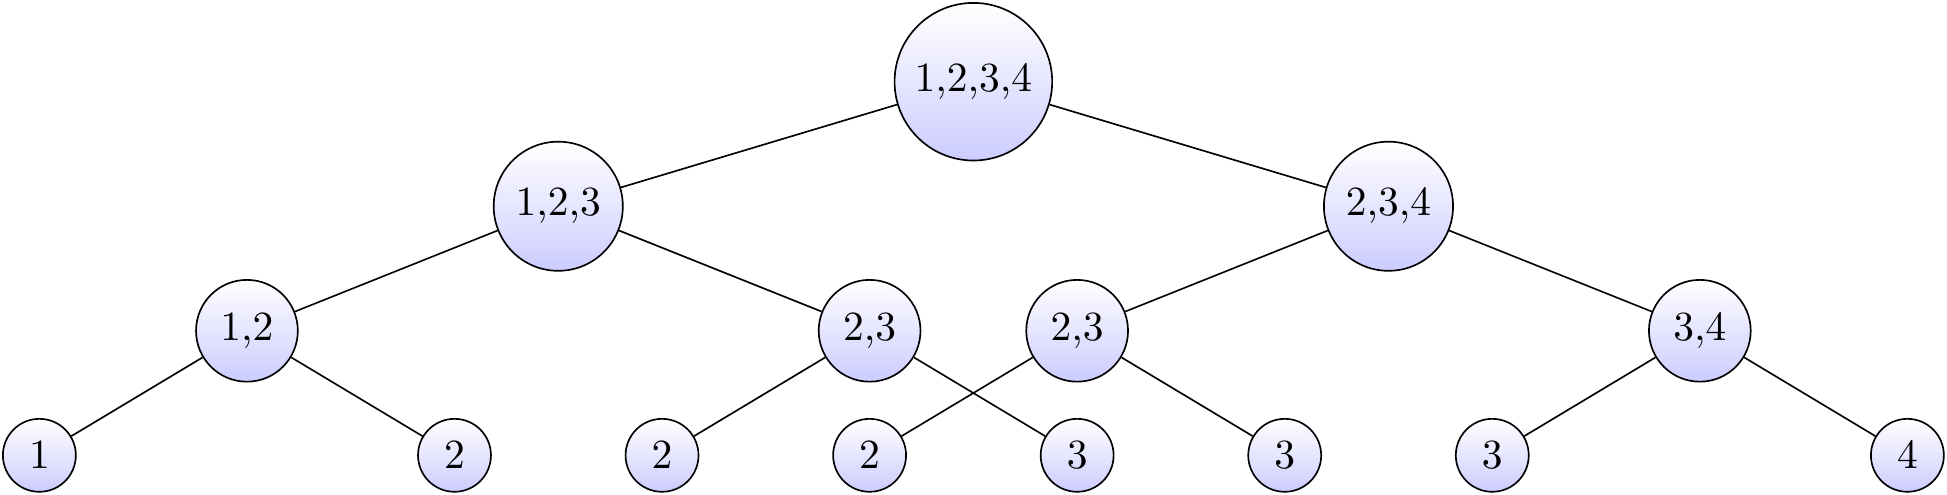
\includegraphics[width=0.9\linewidth]{bookdown-demo_files/figure-latex/unnamed-chunk-4-1} \caption{Some caption.}\label{fig:unnamed-chunk-4}
\end{figure}

\hypertarget{analysis-39}{%
\subsubsection{Analysis}\label{analysis-39}}

The time complexity is exponential, since there are some overlapping subproblems shown in the recursion tree.
\(O(2^{log(n)})\)

\hypertarget{algorithm-39}{%
\subsubsection{Algorithm}\label{algorithm-39}}

\{recursive\}

\hypertarget{java-code---recursion}{%
\subsection{Java Code - Recursion\}}\label{java-code---recursion}}

\begin{Shaded}
\begin{Highlighting}[]
\DataTypeTok{int} \FunctionTok{solution}\NormalTok{(}\DataTypeTok{int}\NormalTok{[] array) \{}
    \KeywordTok{return} \FunctionTok{rec}\NormalTok{(array, }\DecValTok{1}\NormalTok{);}
\NormalTok{\}}

\DataTypeTok{int} \FunctionTok{rec}\NormalTok{(}\DataTypeTok{int}\NormalTok{[] array, }\DataTypeTok{int}\NormalTok{ multiplier) \{}
    \DataTypeTok{int}\NormalTok{ len = array.}\FunctionTok{length}\NormalTok{;}

    \KeywordTok{if}\NormalTok{(len == }\DecValTok{1}\NormalTok{) \{}
        \KeywordTok{return}\NormalTok{ array[}\DecValTok{0}\NormalTok{] * multiplier;}
\NormalTok{    \}}

    \DataTypeTok{int}\NormalTok{ left = array[}\DecValTok{0}\NormalTok{] * multiplier + }\FunctionTok{rec}\NormalTok{(}\BuiltInTok{Arrays}\NormalTok{.}\FunctionTok{copyOfRange}\NormalTok{(array, }\DecValTok{1}\NormalTok{, len), multiplier + }\DecValTok{1}\NormalTok{);}
    \DataTypeTok{int}\NormalTok{ right = array[len - }\DecValTok{1}\NormalTok{] * multiplier + }\FunctionTok{rec}\NormalTok{(}\BuiltInTok{Arrays}\NormalTok{.}\FunctionTok{copyOfRange}\NormalTok{(array, }\DecValTok{0}\NormalTok{, len - }\DecValTok{1}\NormalTok{), multiplier + }\DecValTok{1}\NormalTok{);}

    \KeywordTok{return} \BuiltInTok{Math}\NormalTok{.}\FunctionTok{max}\NormalTok{(left, right);}
\NormalTok{\}}
\end{Highlighting}
\end{Shaded}

\hypertarget{solution---recursion-with-memoization}{%
\subsection{Solution - Recursion with Memoization\}}\label{solution---recursion-with-memoization}}

\hypertarget{walkthrough-37}{%
\subsubsection{Walkthrough}\label{walkthrough-37}}

We can derive \(multiplier = 1 + n - (j - i), 0 \le i < j \le n,\)

The sum of product array{[}i:j{]} is either computed directly (the base case), or it can be computed in constant time from
the already known sum of array{[}i+1:j{]} and array{[}i:j-1{]}.

\hypertarget{analysis-40}{%
\subsubsection{Analysis}\label{analysis-40}}

If we use dynamic programming and memorize all of these subresults, we will get an algorithm with \(O(n^2)\) time
complexity.

\hypertarget{algorithm-40}{%
\subsubsection{Algorithm}\label{algorithm-40}}

\{recursive\}, \{memo\}

\hypertarget{java-code---recursion-with-memoization}{%
\subsection{Java Code - Recursion with Memoization\}}\label{java-code---recursion-with-memoization}}

\begin{Shaded}
\begin{Highlighting}[]
\DataTypeTok{int} \FunctionTok{solution}\NormalTok{(}\DataTypeTok{int}\NormalTok{[] array) \{}
    \DataTypeTok{int}\NormalTok{ len = array.}\FunctionTok{length}\NormalTok{;}
    \DataTypeTok{int}\NormalTok{[][] dp = }\KeywordTok{new} \DataTypeTok{int}\NormalTok{[len + }\DecValTok{1}\NormalTok{][len + }\DecValTok{1}\NormalTok{];}

    \KeywordTok{return} \FunctionTok{memoization}\NormalTok{(array, }\DecValTok{0}\NormalTok{, len, dp);}
\NormalTok{\}}

\CommentTok{// 0 <= start < stop <= n}
\CommentTok{// start inclusive, stop exclusive}
\DataTypeTok{int} \FunctionTok{memoization}\NormalTok{(}\DataTypeTok{int}\NormalTok{[] array, }\DataTypeTok{int}\NormalTok{ start, }\DataTypeTok{int}\NormalTok{ stop, }\DataTypeTok{int}\NormalTok{[][] dp) \{}
    \DataTypeTok{int}\NormalTok{ multiplier = }\DecValTok{1}\NormalTok{ + array.}\FunctionTok{length}\NormalTok{ - (stop - start);}

    \KeywordTok{if}\NormalTok{(dp[start][stop] > }\DecValTok{0}\NormalTok{) \{}
        \CommentTok{//visited subproblem}
        \KeywordTok{return}\NormalTok{ dp[start][stop];}
\NormalTok{    \}}

    \KeywordTok{if}\NormalTok{(stop - start == }\DecValTok{1}\NormalTok{) \{}
        \KeywordTok{return}\NormalTok{ array[start] * multiplier;}
\NormalTok{    \}}

    \DataTypeTok{int}\NormalTok{ left = multiplier * array[start] + }\FunctionTok{memoization}\NormalTok{(array, start + }\DecValTok{1}\NormalTok{, stop, dp);}
    \DataTypeTok{int}\NormalTok{ right = multiplier * array[stop - }\DecValTok{1}\NormalTok{] + }\FunctionTok{memoization}\NormalTok{(array, start, stop - }\DecValTok{1}\NormalTok{, dp);}

    \DataTypeTok{int}\NormalTok{ result = }\BuiltInTok{Math}\NormalTok{.}\FunctionTok{max}\NormalTok{(left, right);}

\NormalTok{    dp[start][stop] = result;}

    \KeywordTok{return}\NormalTok{ result;}
\NormalTok{\}}
\end{Highlighting}
\end{Shaded}

\hypertarget{solution---dynamic-programming-with-tabulation}{%
\subsection{Solution - Dynamic Programming with Tabulation\}}\label{solution---dynamic-programming-with-tabulation}}

\hypertarget{walkthrough-38}{%
\subsubsection{Walkthrough}\label{walkthrough-38}}

We can derive \(multiplier = 1 + n - (j - i), 0 \le i < j \le n,\)

As an alternative, we can use tabulation and start by filling up the memo table. Note that the order of computation
matters: to compute the value memo{[}i{]}{[}j{]}, the values of memo{[}i+1{]}{[}j{]} and memo{[}i{]}{[}j-1{]} must first be known.

Here is the final view of table from the example:

\begin{verbatim}
0   4   11  20  30
0   0   8   18  29
0   0   0   12  25
0   0   0   0   16
0   0   0   0   0
\end{verbatim}

\hypertarget{analysis-41}{%
\subsubsection{Analysis}\label{analysis-41}}

\hypertarget{algorithm-41}{%
\subsubsection{Algorithm}\label{algorithm-41}}

\{dp\}, \{table\}

\hypertarget{java-code---dynamic-programming-with-tabulation}{%
\subsection{Java Code - Dynamic Programming with Tabulation\}}\label{java-code---dynamic-programming-with-tabulation}}

\begin{verbatim}
int solution(int[] array) {
    int len = array.length;
    int[][] dp = new int[len + 1][len + 1];

    return tabulation(array, dp, len);
}

int tabulation(int[] array, int[][] dp, int len) {
    for(int i = 0; i < len; i++) {
        dp[i][i + 1] = len * array[i];
    }

    for (int i = len - 1; i >= 0; i--) {
        for(int j = i + 2; j <= len; j++) {
            int multiplier = 1 + len - (j - i);
            int left = multiplier * array[i] + dp[i + 1][j];
            int right = multiplier * array[j - 1] + dp[i][j - 1];
            int result = Math.max(left, right);
            dp[i][j] = result;
        }
    }

    return dp[0][len];
}
\end{verbatim}

\hypertarget{shortest-word-distance}{%
\section{Shortest Word Distance / / \}}\label{shortest-word-distance}}

\hypertarget{description-38}{%
\subsection{Description}\label{description-38}}

Given a list of words and two words word1 and word2, return the shortest distance between these two words in the list.

\hypertarget{example-37}{%
\subsection{Example}\label{example-37}}

words = {[}``practice'', ``makes'', ``perfect'', ``coding'', ``makes''{]}

word1 = ``coding'', word2=``practice'' result is 3

word1 = ``makes'', word2=``coding'' result is 1

\hypertarget{solution-30}{%
\subsection{Solution}\label{solution-30}}

\hypertarget{walkthrough-39}{%
\subsubsection{Walkthrough}\label{walkthrough-39}}

Record the indices for each word. Retrieve the minimum distance between two group of indices.

\hypertarget{analysis-42}{%
\subsubsection{Analysis}\label{analysis-42}}

Each word in the list is visited once, and each index in both list is visited once. Thus time complexity is O(n),
where the Auxiliary Space is O(n) for storing indices.

\hypertarget{algorithm-42}{%
\subsubsection{Algorithm}\label{algorithm-42}}

\hypertarget{java-code-33}{%
\subsection{Java Code}\label{java-code-33}}

\begin{Shaded}
\begin{Highlighting}[]
\KeywordTok{public} \DataTypeTok{int} \FunctionTok{shortestDistance}\NormalTok{(}\BuiltInTok{String}\NormalTok{[] words, }\BuiltInTok{String}\NormalTok{ word1, }\BuiltInTok{String}\NormalTok{ word2) \{}
    \CommentTok{// list of indices for word1 and word2 in the array respectively.}
    \BuiltInTok{List}\NormalTok{<}\BuiltInTok{Integer}\NormalTok{> list1 = }\KeywordTok{new} \BuiltInTok{ArrayList}\NormalTok{<>();}
    \BuiltInTok{List}\NormalTok{<}\BuiltInTok{Integer}\NormalTok{> list2 = }\KeywordTok{new} \BuiltInTok{ArrayList}\NormalTok{<>();}

    \KeywordTok{for}\NormalTok{(}\DataTypeTok{int}\NormalTok{ i = }\DecValTok{0}\NormalTok{; i < words.}\FunctionTok{length}\NormalTok{; i++) \{}
        \KeywordTok{if}\NormalTok{(words[i].}\FunctionTok{equals}\NormalTok{(word1)) \{}
\NormalTok{            list1.}\FunctionTok{add}\NormalTok{(i);}
\NormalTok{        \} }\KeywordTok{else} \KeywordTok{if}\NormalTok{(words[i].}\FunctionTok{equals}\NormalTok{(word2)) \{}
\NormalTok{            list2.}\FunctionTok{add}\NormalTok{(i);}
\NormalTok{        \}}
\NormalTok{    \}}

    \DataTypeTok{int}\NormalTok{ min = words.}\FunctionTok{length}\NormalTok{;}
    \KeywordTok{for}\NormalTok{(}\DataTypeTok{int}\NormalTok{ i = }\DecValTok{0}\NormalTok{, j = }\DecValTok{0}\NormalTok{; i < list1.}\FunctionTok{size}\NormalTok{() && j < list2.}\FunctionTok{size}\NormalTok{();) \{}
        \DataTypeTok{int}\NormalTok{ index1 = list1.}\FunctionTok{get}\NormalTok{(i);}
        \DataTypeTok{int}\NormalTok{ index2 = list2.}\FunctionTok{get}\NormalTok{(i);}

\NormalTok{        min = }\BuiltInTok{Math}\NormalTok{.}\FunctionTok{min}\NormalTok{(min, }\BuiltInTok{Math}\NormalTok{.}\FunctionTok{abs}\NormalTok{(index1 - index2));}

        \KeywordTok{if}\NormalTok{(index1 < index2) \{}
\NormalTok{            i++;}
\NormalTok{        \} }\KeywordTok{else} \KeywordTok{if}\NormalTok{(index1 > index2) \{}
\NormalTok{            j++;}
\NormalTok{        \} }\KeywordTok{else}\NormalTok{ \{}
            \CommentTok{// comparing the same indices}
            \KeywordTok{return} \DecValTok{0}\NormalTok{;}
\NormalTok{        \}}
\NormalTok{    \}}

    \KeywordTok{return}\NormalTok{ min;}
\NormalTok{\}}
\end{Highlighting}
\end{Shaded}

\hypertarget{literature}{%
\chapter{Literature}\label{literature}}

Here is a review of existing methods.

\hypertarget{two-sum-iv---input-is-a-bst-leetcode-653-easy-1}{%
\section{Two Sum IV - Input is a BST / LeetCode 653 / Easy}\label{two-sum-iv---input-is-a-bst-leetcode-653-easy-1}}

\hypertarget{description-39}{%
\subsection{Description}\label{description-39}}

Given a Binary Search Tree and a target number, return true if there exist two elements in the BST such that their sum
is equal to the given target.

\hypertarget{example-38}{%
\subsection{Example}\label{example-38}}

\begin{figure}
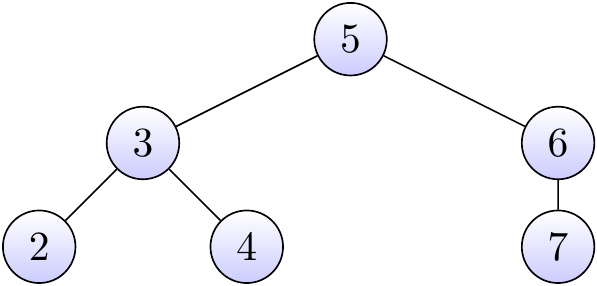
\includegraphics[width=0.9\linewidth]{bookdown-demo_files/figure-latex/unnamed-chunk-5-1} \caption{Some caption.}\label{fig:unnamed-chunk-5}
\end{figure}

\textbackslash{}Target = 9, Output = True.

\hypertarget{solution-31}{%
\subsection{Solution\}}\label{solution-31}}

\hypertarget{walkthrough-40}{%
\subsubsection{Walkthrough\}\textbackslash{}}\label{walkthrough-40}}

Use a HashSet to store value of current node, that is (node.val). Then check if answer = (target - node.val)
and return true if existed; otherwise, recursively call the same function for its left and right children.

\hypertarget{analysis-43}{%
\subsubsection{Analysis}\label{analysis-43}}

Time complexity is O(n) since every node is visited. Auxiliary Space is O(1)

\hypertarget{algorithm-43}{%
\subsubsection{Algorithm}\label{algorithm-43}}

recursive

\hypertarget{java-code-34}{%
\subsection{Java Code}\label{java-code-34}}

\begin{Shaded}
\begin{Highlighting}[]
\KeywordTok{public} \DataTypeTok{boolean} \FunctionTok{findTarget}\NormalTok{(}\BuiltInTok{TreeNode}\NormalTok{ root, }\DataTypeTok{int}\NormalTok{ target) \{}
    \BuiltInTok{Set}\NormalTok{<}\BuiltInTok{Integer}\NormalTok{> set = }\KeywordTok{new} \BuiltInTok{HashSet}\NormalTok{<>();}
    \KeywordTok{return} \FunctionTok{findTarget}\NormalTok{(root, target, set);}
\NormalTok{\}}

\KeywordTok{public} \DataTypeTok{boolean} \FunctionTok{findTarget}\NormalTok{(}\BuiltInTok{TreeNode}\NormalTok{ node, }\DataTypeTok{int}\NormalTok{ target, }\BuiltInTok{Set}\NormalTok{<}\BuiltInTok{Integer}\NormalTok{> set) \{}
    \KeywordTok{if}\NormalTok{(node == }\KeywordTok{null}\NormalTok{) \{}
        \KeywordTok{return} \KeywordTok{false}\NormalTok{;}
\NormalTok{    \} }\KeywordTok{else} \KeywordTok{if}\NormalTok{(set.}\FunctionTok{contains}\NormalTok{(target - node.}\FunctionTok{val}\NormalTok{)) \{}
        \KeywordTok{return} \KeywordTok{true}\NormalTok{;}
\NormalTok{    \} }\KeywordTok{else}\NormalTok{ \{}
        \CommentTok{//recursively calling}
\NormalTok{        set.}\FunctionTok{add}\NormalTok{(node.}\FunctionTok{val}\NormalTok{);}
        \KeywordTok{return} \FunctionTok{findTarget}\NormalTok{(node.}\FunctionTok{right}\NormalTok{, target, set) || }\FunctionTok{findTarget}\NormalTok{(node.}\FunctionTok{left}\NormalTok{, target, set);}
\NormalTok{    \}}

\NormalTok{\}}
\end{Highlighting}
\end{Shaded}

\hypertarget{methods}{%
\chapter{Methods}\label{methods}}

We describe our methods in this chapter.

\hypertarget{applications}{%
\chapter{Applications}\label{applications}}

Some \emph{significant} applications are demonstrated in this chapter.

\hypertarget{example-one}{%
\section{Example one}\label{example-one}}

\hypertarget{example-two}{%
\section{Example two}\label{example-two}}

\hypertarget{final-words}{%
\chapter{Final Words}\label{final-words}}

We have finished a nice book.

\bibliography{latex/book.bib,latex/packages.bib}

\end{document}
